\chapter{Investigating the Molecular Mechanisms of Tension-dependent Re-localisation of Shugoshin}

\section{Introduction}
Centromere executes its function of coordinating chromosome segregation partially by controlling the subcellular location of critical regulators. A remarkable example is the tension-dependent re-localisation of shugoshin. 

To be segregated into different daughter cells later, sister chromatids need to be bipolarly attached to the spindle in mitosis or meiosis II, which is called bi-orientation \citep{Tanaka2010Kinetochore-microtubuleBi-orientation}. Bi-oriented sister chromatids come under tension due to the counteraction between the resistance of cohesion and the pulling of microtubules. Cells sense a lack of tension and destabilise erroneous microtubule-kinetochore attachment, a process termed error correction, meanwhile delaying cell cycle progression until tension is generated \citep{Nicklas1997HowChromosomes, Nicklas1994, Tanaka2010Kinetochore-microtubuleBi-orientation}. The conserved shugoshin protein family is important for the establishment of tension \citep{Watanabe2005, Clift2011, Gutierrez-Caballero2012Shugoshins:Centromere, Marston2015, Zhang2020FunctioningMitosis}. The name itself, 'guardian spirit' in Japanese, comes from its well-conserved canonical function of cohesion protection in meiosis I \citep{Lister2010Age-relatedSgo2, Llano2008Shugoshin-2Mice, Lee2008, Rattani2013Sgol2Oocytes, Marston2004a, Kitajima2004a, Katis2004, Rabitsch2004TwoII, Kerrebrock1992TheDifferentiation, Cromer2013CentromericInterkinesis, Zamariola2014SHUGOSHINsThaliana, Wang2011OsSGO1Meiosis, Hamant2005AFunctions, Ma2021MeikinI, Miyazaki2017HierarchicalI}. In vertebrates, shugoshin also protects centromeric cohesion from Wapl-mediated cohesin removal pathway in mitosis \citep{Rivera2009ShugoshinExtracts, Shintomi2009ReleasingSgo1, Huang2007, Tang2006a, McGuinness2005ShugoshinCells, Kitajima2005, Salic2004VertebrateMitosis, Liang2019ACells}. Shugoshin further assists cohesion protection by directly sequestering separase with the SAC component Mad2\citep{Rattani2013Sgol2Oocytes, Hellmuth2020Securin-independentShugoshinMAD2, Orth2011ShugoshinMad2}. Apart from cohesion protection, shugoshin additionally promotes bi-orientation by facilitating error correction \citep{Meppelink2015Shugoshin-1Bi-orientation, Huang2007, Peplowska2014, Nerusheva2014, Verzijlbergen2014, Tsukahara2010a, Yamagishi2010, Hadders2020UntanglingMitosis, Broad2020AuroraCells, Kawashima2007, Vanoosthuyse2007, Rivera2012} and, at least in yeast, contributing to the geometry of the centromeric region biased towards a shape where sister kinetochores are more easily captured by microtubules from the opposite spindle poles \citep{Indjeian2007, Haase2012Bub1Dynamics, Verzijlbergen2014, Peplowska2014, Sane2021ShugoshinDisassembly}. Despite different molecular details in various species, all these functions are implemented by shugoshin acting as an adaptor recruiting different effector proteins to the centromeric region, including PP2A-B56 \citep{Xu2009StructureInteraction, Ueki2021AMitosis}, CPC \citep{Abad2022MechanisticCPC}, MCAK \citep{Tanno2010} and condensin \citep{Verzijlbergen2014, Yahya2020}. 

Interestingly, the location of shugoshin has been found to change in response to tension across species. Human Sgo1 and Sgo2 redistribute from the inner centromere towards the kinetochore upon tension establishment in mitosis \citep{Huang2007, Lee2008, Liu2013, Asai2020}. Mouse Sgo2 follows the same pattern in meiosis II \citep{Lee2008, Gomez2007}. In budding yeast, tension removes its only shugoshin protein Sgo1 from peri-centromere \citep{Eshleman2014, Nerusheva2014, Paldi2020ConvergentPericentromeres}. Although the effect of tension has not been directly studied, locations are different between metaphase and anaphase for \textit{Drosophila} MEI-S332 (mitosis and meiosis II) and fission yeast Sgo2 (mitosis) \citep{Clarke2005, Kawashima2007}, raising the possibility that they also undergo tension-dependent re-localisation. 

Re-localisation of shugoshin is functionally relevant. It has been proposed as key to tension sensing \citep{Marston2015}. Screening in budding yeast identified Sgo1 being required to delay anaphase onset in the absence of tension \citep{Indjeian2005a}. Later, it was shown to be due to its role in preventing SAC silencing \citep{Jin2013TheAttachment}. Given the function of Sgo1 to support CPC localisation, it was reasoned that tension-dependent re-localisation of Sgo1 triggers the removal of CPC from the centromere, leading to SAC silencing \citep{Nerusheva2014}. In support of this model, artificially tethering Sgo1 to the kinetochore caused prolonged metaphase \citep{Su2021SumoylationAnaphase}. In mammals, the re-localisation is thought to inactivate cohesin protection \citep{Lee2008}. Indeed, impaired human Sgo1 re-localisation increased lagging chromosomes in anaphase \citep{Liu2013}. Besides, at least in budding yeast, the re-localisation of shugoshin might be the signal for chromosome condensation. The key condensation player condensin spreads from the centromere to chromosome arms in a tension-dependent manner \citep{Leonard2015}. As its interactor with a similar response to tension, Sgo1 potentially mediates the spread. Consistent with this idea, mitotic chromosome condensation is abolished in \textit{sgo1} mutant \citep{Kruitwagen2018}. 

It is well established across species that the SAC component Bub1 kinase at the kinetochore phosphorylates threonine 120 of histone H2A (serine 121 in yeast) around centromeric chromatin, providing a high-affinity marker for shugoshin \citep{Rivera2012, Boyarchuk2007Bub1Centromere, Williams2017Bub1Kinetochores, Kitajima2005, Perera2010, Tang2004, Fernius2007Bub1Mitosis, Kiburz2005, Kawashima2010a}. Nevertheless, the localisation of shugoshin is further regulated by complicated, not fully understood, interplay of various factors through reversible PTMs. In human cells, a step-wise recruitment model of Sgo1 has been proposed \citep{Liu2013, Liu2013a, Liu2015}. Sgo1 is first recruited proximal to the kinetochore due to direct binding to nucleosomes with H2A-pT120. Pol II-mediated centromeric transcription then disengages Sgo1 from nucleosomes, allowing it to reach the inner centromere. Finally, Sgo1 phosphorylated at threonine 346 by CDK is captured by cohesin there. A number of other factors supporting shugoshin localisation have been reported in different species, including HP1 \citep{Yamagishi2008, Kang2011, Perera2010}, CPC \citep{Huang2007, Tanno2010, Rivera2012, Kawashima2007, Boyarchuk2007Bub1Centromere, Resnick2006INCENPDrosophila}, PP2A \citep{Tang2006a}, CENP-A \citep{Petty2018ConnectingCheckpoint, Eot-Houllier2018AuroraFatigue, Mishra2018BuddingChromatin} and H3 \citep{Buehl2018a, Luo2016}, while Polo kinase \citep{Clarke2005}, SET \citep{Qu2019SETSegregation, Krishnan2017Phospho-H1Mitosis}, KAT2A \citep{Petty2018ConnectingCheckpoint} and PP2A \citep{Nerusheva2014} were suggested to de-localise it. 

The mechanism of shugoshin tension-dependent re-localisation is less well understood. \cite{Nerusheva2014} attempted to address it in budding yeast, yet questions are left to be answered. It was proposed that reduced Bub1 activity at peri-centromere by tension leads to the de-phosphorylation of its substrate(s), thus resulting in the removal of Sgo1 (Figure~\ref{fig:naive}). How Bub1 activity in a particular area is regulated by tension remains to be elucidated. Due to technical difficulties, it was unable to directly monitor H2A-pS121 by that time, leaving the effect of tension on it untested. Moreover, this model predicts the existence of at least one phosphatase antagonizing Bub1. Although it was found that PP2A-B56 (Rts1 in budding yeast) negatively regulates Sgo1 enrichment at the peri-centromere, whether it is responsible for Sgo1 de-localisation is unclear. The human model emphasizes phospho-regulation of shugoshin interaction with cohesin by tension underlying its movement from the inner centromere to the kinetochore-proximal region \citep{Liu2013, Liu2015}. It is interesting to explore if this mechanism could be conserved in budding yeast as well. Besides, the exact localisation of human H2A-pT120 by IF is inconsistent in the literature, with reports arguing it covers both the inner centromere \citep{Yamagishi2010} and the kinetochore proximity or it is usually only at the latter \citep{Liu2013}. Due to the repetitive nature of human centromere, the two arguments could not be distinguished by sequence-based technology such as ChIP. Whereas budding yeast can be used to address this question for its point centromere structure. 

\begin{figure}[htbp]
  \centering
  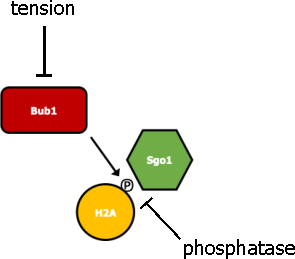
\includegraphics[width=0.3\textwidth]{figures/naive model.pdf}
  \caption[Proposed budding yeast model of tension-dependent re-localisation of Sgo1]{Proposed budding yeast model of tension-dependent re-localisation of Sgo1. Tension causes a reduction of Bub1 phosphorylation capability at peri-centromere, resulting in the de-phosphorylation of the substrates (H2A-S121 is used as an example here) by the counteracting phosphatase. Sgo1 is therefore de-localised from the peri-centromere.}
  \label{fig:naive}
\end{figure} 

\nomenclature{SAC}{Spindle Assembly Checkpoint}
\nomenclature{CPC}{Chromosome Passenger Complex}
\nomenclature{PP2A}{Protein Phosphatase 2A}
\nomenclature{MCAK}{Mitotic Centromere-Associated Kinesin}
\nomenclature{SET}{SET nuclear proto-oncogene}
\nomenclature{CDK}{Cyclin-Dependent Kinase}
\nomenclature{Pol II}{RNA Polymerase II}
\nomenclature{HP1}{Heterochromatin Protein 1}
\nomenclature{KAT2A}{lysine AcetylTransferase 2A}
\nomenclature{PTM}{Post Translational Modification}
\nomenclature{ChIP}{Chromatin ImmunoPrecipitation}
\nomenclature{IF}{ImmunoFluorescence}


\section{Results}
\subsection{Whether tension pulls Bub1 away from the peri-centromere border is inconclusive}
It is unclear how tension inhibits Bub1 activity at the peri-centromere. One possibility is that kinetochore-localised Bub1 is pulled away from its substrates at the peri-centromere because of tension \citep{Nerusheva2014}. This hypothesis is further supported by the study on peri-centromeric chromatin conformation showing that tension reduces the interaction between the core centromere and peri-centromeric borders \citep{Paldi2020ConvergentPericentromeres}, where Sgo1 mainly localises revealed by ChIP-seq \citep{Verzijlbergen2014, Deng2018}. 

To test this idea, I first wanted to measure FRET between Bub1 and nucleosomes. If the hypothesis is true, the FRET signal should decrease in the presence of tension. hence, I constructed a strain bearing \textit{BUB1-mNG HTB1-mCherry pMET-CDC20}. To validate the method, cells were synchronized in G1 and released into a metaphase arrest without tension by nocodazole, as this condition is expected to give a higher FRET signal. Unfortunately, it was unable to detect any FRET signal between Bub1 and Htb1, leaving the method usable (Figure~\ref{fig:FRET}). The problem is possibly due to the low expression of Bub1 protein and the small size of budding yeast. 
\nomenclature{FRET}{Förster Resonance Energy Transfer}

\begin{figure}[htbp]
  \centering
  \includesvg[width=0.6\textwidth]{figures/Bub1-mNG Htb1-mCherry FRET.svg}
  \caption[Representative image of FRET between Bub1-mNG and Htb1-mCherry of metaphase cells without tension]{Representative image of FRET between Bub1-mNG and Htb1-mCherry of metaphase cells without tension. Bleed-through from both fluorophores to the FRET channel are subtracted. }
  \label{fig:FRET}
\end{figure} 

As an alternative approach, I decided to directly measure the distance between Bub1 and peri-centromeric borders, which is expected to increase by tension. To this end, I labelled one peri-centromeric border of chromosome I using the Tet-On system, with a tetO array on the locus and tetR-tdTomato under a constitutive promoter. Cells bearing \textit{BUB1-mNG pMET-CDC20} and the labelled peri-centromeric border of chromosome I were synchronized in G1 and released into methionine-containing media for a metaphase arrest with tension. Time-lapse live-cell imaging was performed since the G1 release. Bub1-mNG appears as one focus as cells enter the S phase, indicated by the appearance of small buds. This is due to centromere clustering in budding yeast \citep{Taddei2012StructureNucleus}. All kinetochores  are seen together as one dot under current light microscopes. Bub1-mNG then splits into two foci due to sister kinetochores separating by tension. On the other hand, tetR-tdTomato stays as one focus from the beginning of imaging. Occasionally, it splits into two foci after the separation of Bub1-mNG foci (Figure~\ref{fig:periCEN}A). The distance between Bub1-mNG and tetR-tdTomato focus $L$ was measured. After the separation of Bub1-mNG, there could be two $L$s in one cell. I arbitrarily named the shorter one as $L_{1}$ and the longer one as $L_{2}$. The inter-kinetochore distance measured from the distance between Bub1-mNG dots was used as the indicator of tension. Before Bub1-mNG separation, $L$ ranges from 0.01 to 1.19 \si{\micro\metre} with a median of 0.32 \si{\micro\metre}. After Bub1-mNG separation, $L_{1}$ and $L_{2}$ together gave a data set showing a slight increase, ranging from 0.01 to 1.24 \si{\micro\metre} with a median of 0.40 \si{\micro\metre}. However, if analysed individually, $L_{1}$ is not correlated with the inter-kinetochore distance ($R^2 = 0.03$) despite $L_{2}$ shows a moderated correlation ($R^2 = 0.59$) (Figure~\ref{fig:periCEN}B).This result suggests the distance between one of the Bub1-mNG foci and the peri-centromere border is independent of tension, arguing against the hypothesis of Bub1 being pulled further away from its substrates at the peri-centromere. Whereas the other Bub1-mNG focus does become further, favouring the hypothesis. Therefore, whether tension pulls Bub1 away from the peri-centromere border is inconclusive. 


\begin{figure}[htbp]
  \centering
  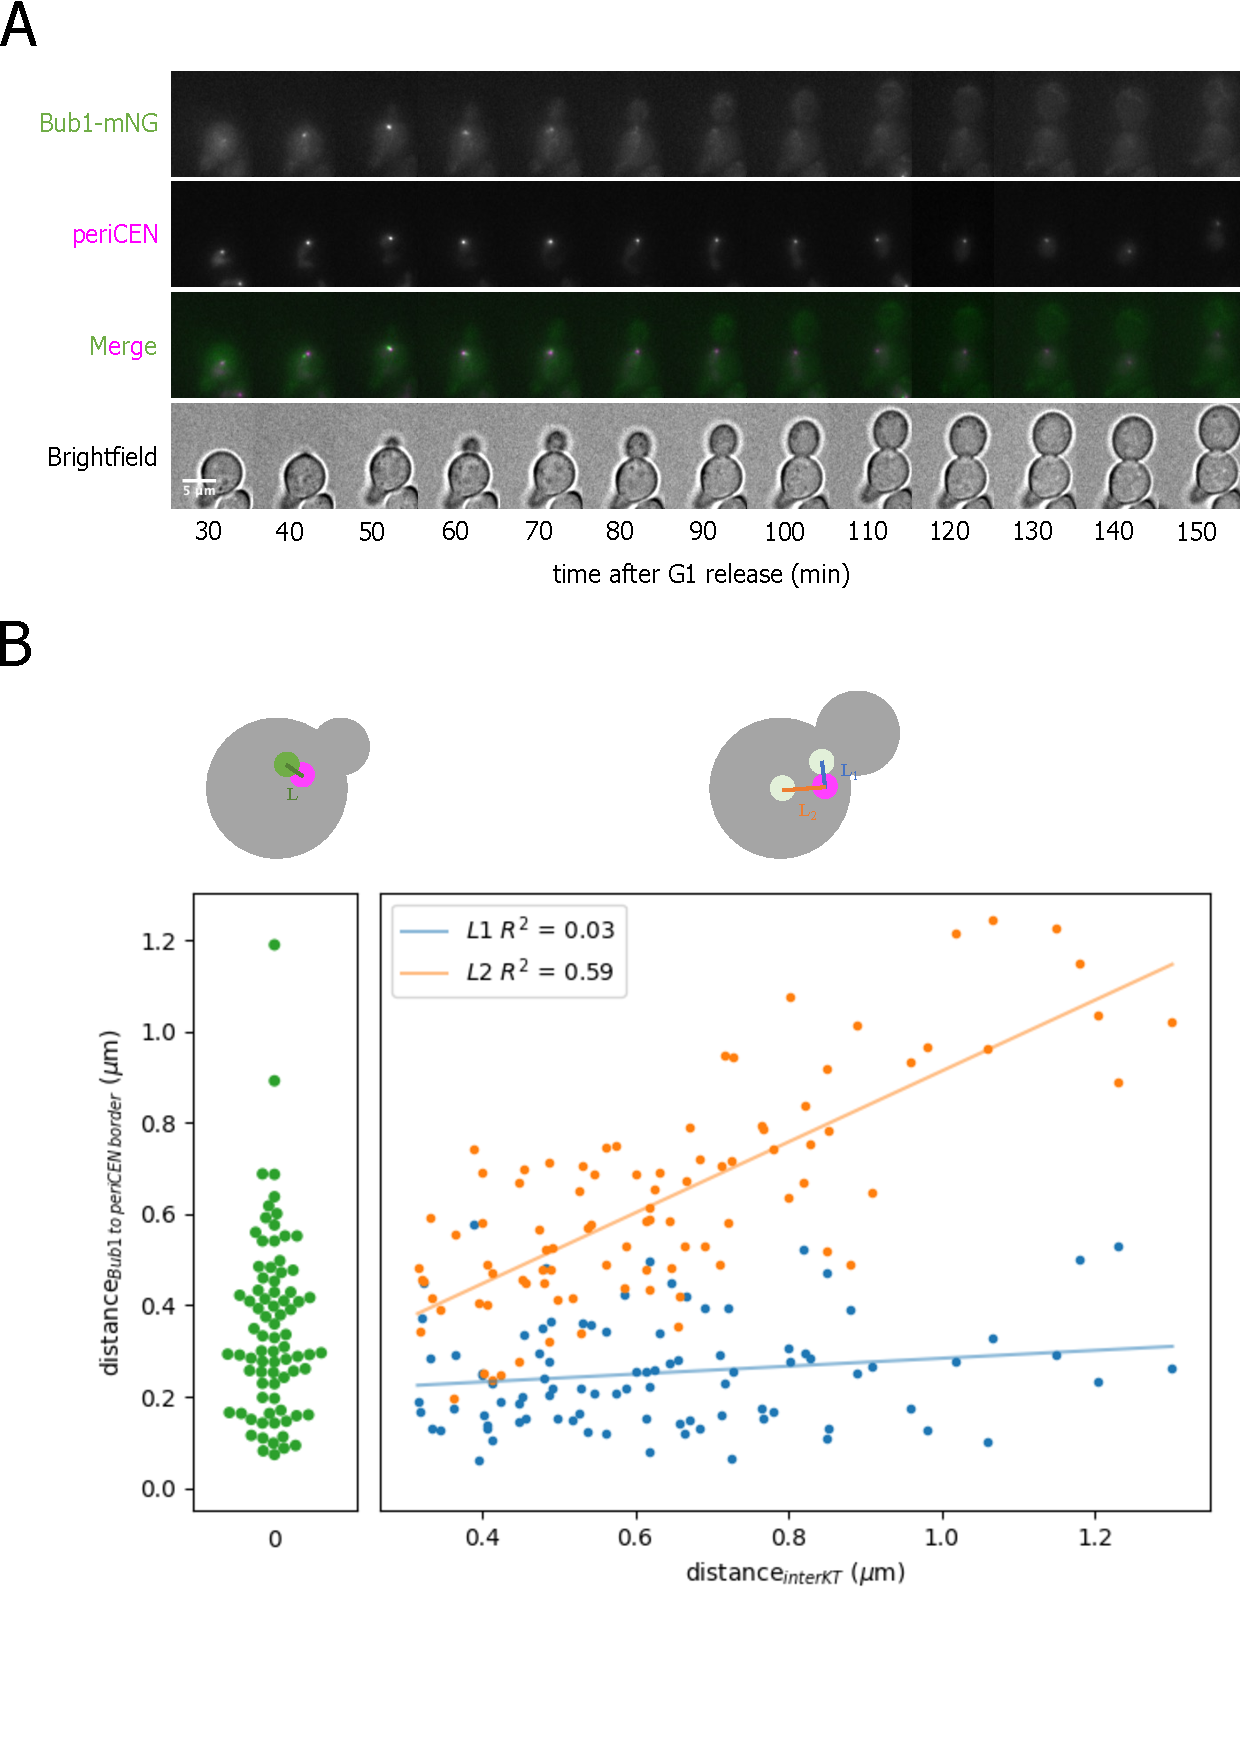
\includegraphics[width=0.9\textwidth]{figures/Bub1-mNG peri-cen.pdf}
  \caption[The shorter distance between Bub1 and peri-centromere is independent of the inter-kinetochore distance]{The shorter distance between Bub1 and peri-centromere is independent of the inter-kinetochore distance. (A) Montage of representative time-lapse imaging. (B) Scatter plot showing the relation of Bub1-to-peri-centromere distance and inter-kinetochore distance. N=30 cells were followed over time and quantified for $L$ (the distance before Bub1-mNG separation), $L_{1}$ (the shorter distance after Bub1-mNG separation) and $L_{2}$ (the longer distance after Bub1-mNG separation), which are presented in green, orange and blue, respectively. The line with the same colour represents the model of simple linear regression. }
  \label{fig:periCEN}
\end{figure} 

\nomenclature{mNG}{mNeonGreen}

\subsection{Bub1 is de-localised from the kinetochore by tension}
During data analysis of the previous experiment, I noticed a reduction in fluorescence intensity of Bub1-mNG foci as they separate to an extent that they are barely visible at the end of imaging. This cannot be simply explained by photo-bleaching because tdTomato is supposed to have a shorter bleaching time than mNG, yet it remains visible (Figure~\ref{fig:periCEN}A). The observation raises the possibility that the kinetochore localisation of Bub1 could be under the regulation of tension, leading to the physical separation from its substrates. The idea that Bub1 localisation could be regulated by tension has been implicated in literature \citep{Asai2020, Proudfoot2019, Jin2017PrematureCerevisiae}. To test this, I wanted to quantify the dynamics of the amount of Bub1 at the kinetochore as well as the inter-kinetochore distance. Since Bub1-mNG becomes indistinguishable from the background after separation, I chose to use the outer-kinetochore protein Mtw1 as a more reliable measure of the inter-kinetochore distance. I constructed a strain bearing \textit{BUB1-mNG MTW1-tdTomato pMET-CDC20}. Time-lapse live-cell imaging was again performed since the G1 release (Figure~\ref{fig:bub1mtw1}A). As expected, Bub1-mNG follows the same dynamics as in the previous experiment. While Mtw1-tdTomato appears as one focus at the start of imaging and then splits into two foci as the cell cycle progresses (Figure~\ref{fig:bub1mtw1}B). Further quantification showed that the fluorescence intensity of kinetochore Bub1-mNG peaks at 60 \si{\minute} since G1 release, with an over 2-fold decrease at 70 \si{\minute}, coinciding with the beginning of Mtw1-tdTomato foci separation (Figure~\ref{fig:bub1mtw1}C). This indicates that kinetochore-localised Bub1 is reduced upon the establishment of bi-orientation. 

\begin{figure}[htbp]
  \centering
  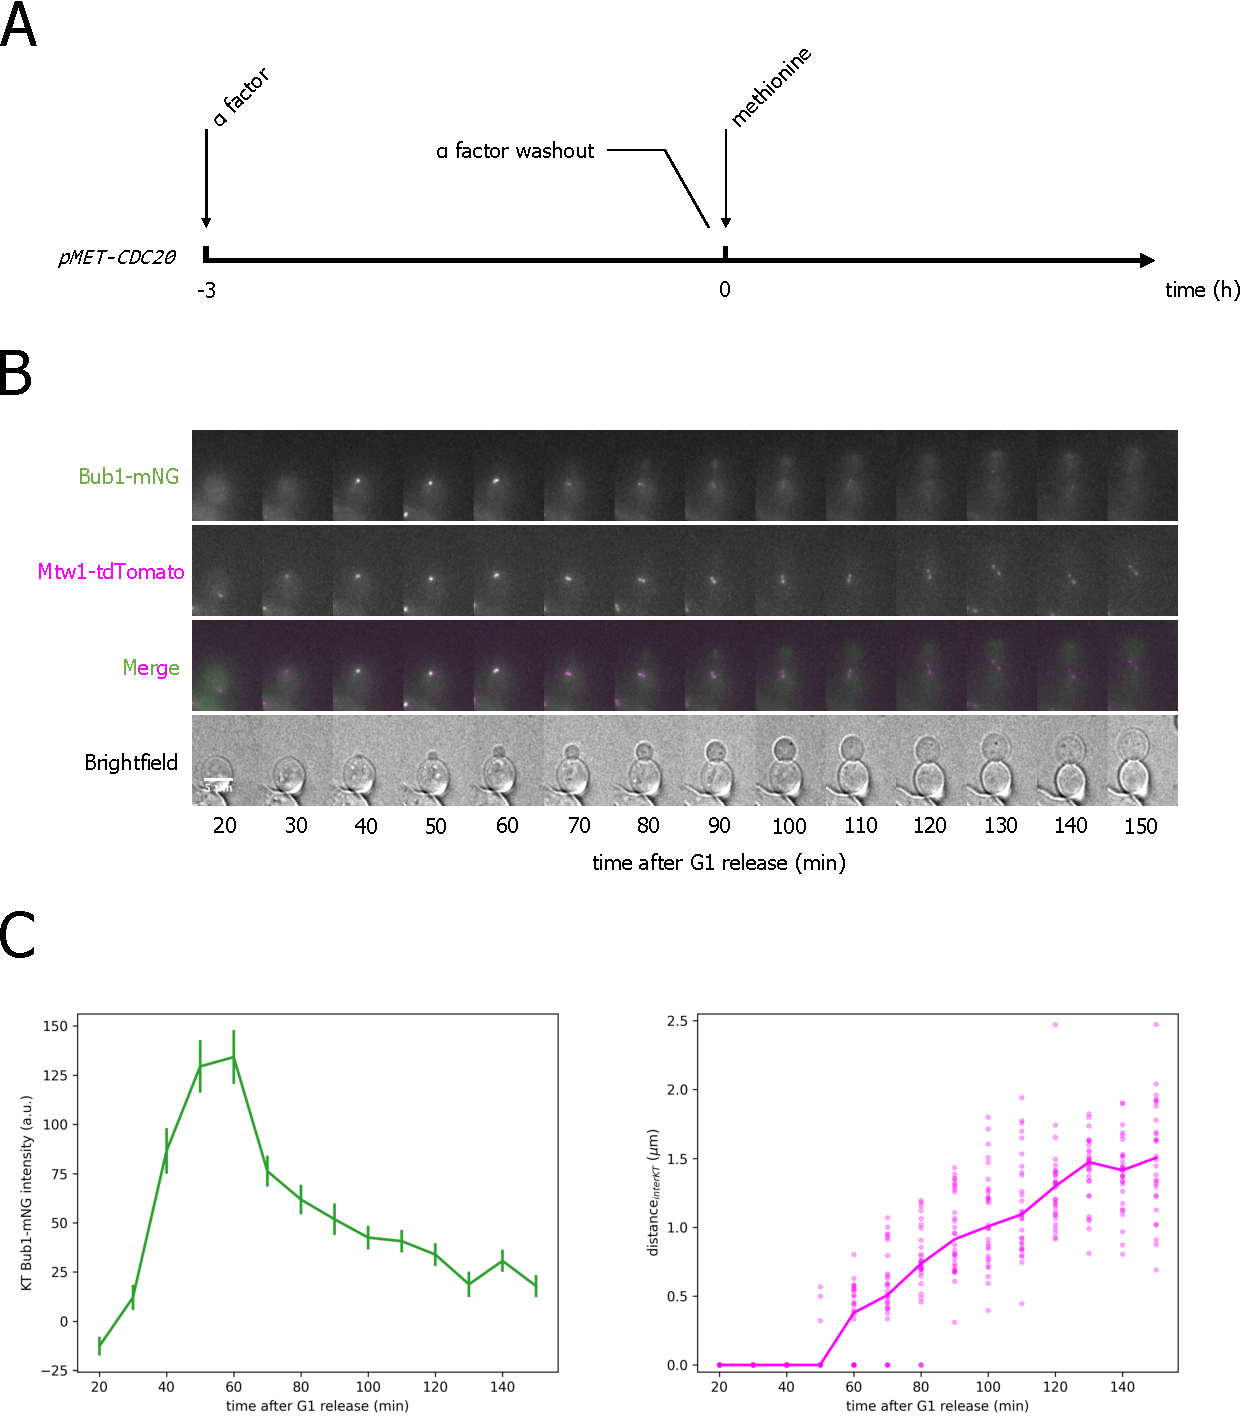
\includegraphics[width=0.9\textwidth]{figures/Bub1-mNG vs Mtw1-td.pdf}
  \caption[Kinetochore-localised Bub1 is reduced upon bi-orientation]{Kinetochore-localised Bub1 is reduced upon bi-orientation. (A) Schematics of experimental procedures. (B) Montage of representative time-lapse imaging. (C) N=30 cells were followed over time and quantified for kinetochore Bub1-mNG fluorescence intensity and inter-kinetochore distance. Left panel: mean fluorescence intensity of Bub1-mNG at the kinetochore as a function of time. The error bar represents the standard error. Right panel: Median inter-kinetochore distance as a function of time. Individual data points are shown as dots. }
  \label{fig:bub1mtw1}
\end{figure} 

I then sought to test whether the reduction in Bub1 kinetochore localisation is due to protein degradation or re-localisation. Human Bub1 is degraded by APC in anaphase \citep{Qi2007KEN-box-dependentComplex/cyclosome} but it is not known in budding yeast. Hence, I performed a synchronised mitotic time course experiment followed by western blotting to check Bub1 protein expression. Cells bearing \textit{BUB1-6HA} were synchronised in G1 and released into rich media. $\alpha$ factor was added 60 \si{\minute} after the release to arrest cells in the next G1 (Figure~\ref{fig:bub1timecourse}A). Tubulin IF was used to examine the progression of the cell cycle. At 75 \si{\minute} after G1 release, over 80\% of cells were in metaphase while most cells were in anaphase at 90 and 105 \si{\minute} (Figure~\ref{fig:bub1timecourse}B). Western blotting with anti-HA antibody showed Bub1 protein level reached its apex at 90 \si{\minute} and started to decrease since 105 \si{\minute} (Figure~\ref{fig:bub1timecourse}C), suggesting Bub1 is degraded in late anaphase in budding yeast. Therefore, protein degradation could not be the reason for reduced Bub1 kinetochore localisation in metaphase in the previous experiment. Interestingly, Bub1 experienced changes in electrophoretic mobility at the early stage of the cell cycle, indicating its phosphorylation status might be actively regulated. As this is beyond the scope of my project, this was not investigated further. 

\begin{figure}[htbp]
  \centering
  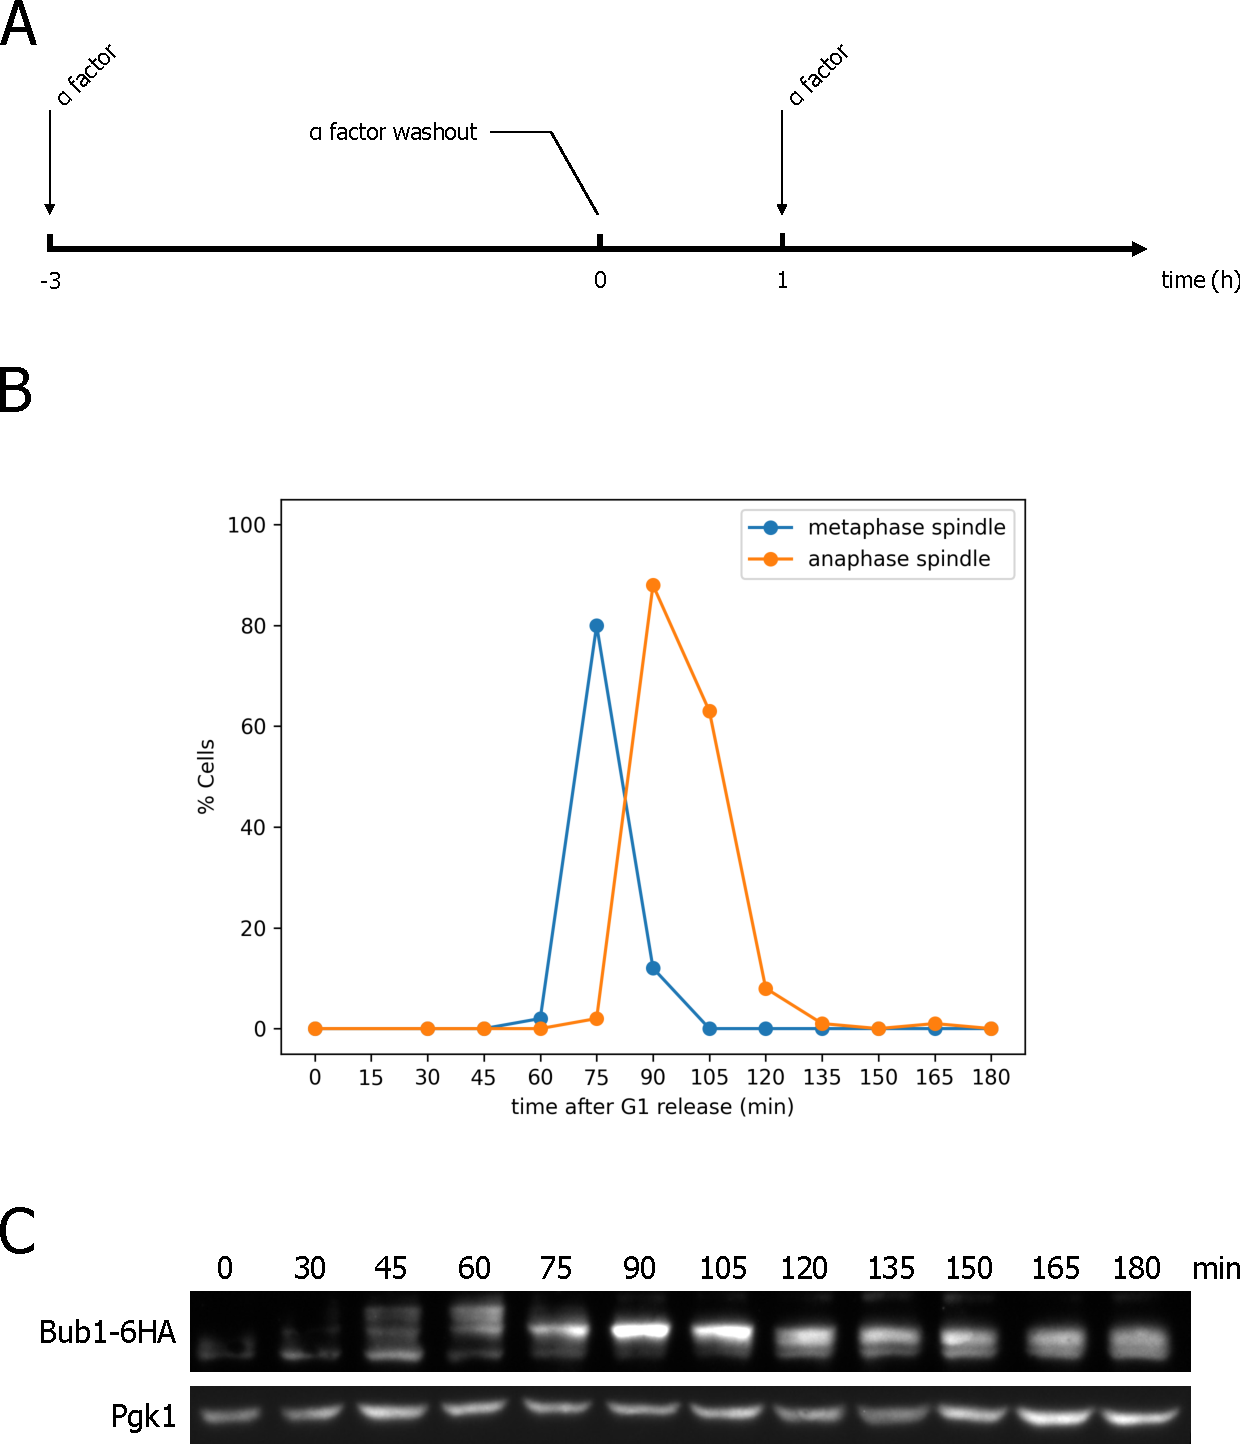
\includegraphics[width=0.9\textwidth]{chapter3/figures/Bub1-6HA time course.pdf}
  \caption[Bub1 is not degraded until anaphase]{Bub1 is not degraded until anaphase. (A) Schematics of experimental procedures. (B) The proportion of cells with metaphase or anaphase spindle over time by tubulin IF. (C) Western blotting with anti-HA antibody to detect Bub1 protein. Pgk1 was used as the loading control.}
  \label{fig:bub1timecourse}
\end{figure} 

The experiments above suggest that Bub1 is re-localised from the kinetochore upon bi-orientation. Given that both tension and kinetochore-microtubule attachment are established in this case, it is unkown whether tension is required for Bub1 de-localisation besides attachment. To abolish tension without disrupting attachment, I decided to disable sister chromatid cohesion by depleting the kleisin subunit Scc1 of the cohesin complex. Cells from Figure~\ref{fig:bub1mtw1} with or without additional \textit{pMET-SCC1} were synchronised in G1. Methionine was added 45 \si{\minute} before releasing to pre-clean Scc1 in the \textit{pMET-SCC1} strain. Live-cell imaging was performed to quantify kinetochore Bub1-mNG fluorescence intensity and inter-kinetochore distance (Figure~\ref{fig:bub1metscc1}A). As expected, the \textit{pMET-SCC1} strain exhibited increased inter-kinetochore distance ($\sim$2.5 \si{\micro\metre} towards the end of the experiment) compared to the wild type ($\sim$1.5 \si{\micro\metre} towards the end of the experiment), indicating a reduction in sister chromatid cohesion. Unlike the wild type, the signal of kinetochore Bub1-mNG is maintained at a similar value after 60 \si{\minute} from G1 release in the \textit{pMET-SCC1} strain (Figure~\ref{fig:bub1metscc1}B and C), suggesting Bub1 is not removed from the kinetochore in the absence of tension while no additional disruption was applied on attachment. To rule out the potential artefacts from \textit{pMET-SCC1} causing an increase in Bub1 expression, I used western blotting to check the Bub1 protein expression level in the wild type and the \textit{pMET-SCC1} strain arrested in metaphase by methionine depletion. No obvious difference was observed (Figure~\ref{fig:bub1metscc1}D). Hence, the kinetochore localisation of Bub1 is reduced by tension. 

\begin{figure}[htbp]
  \centering
  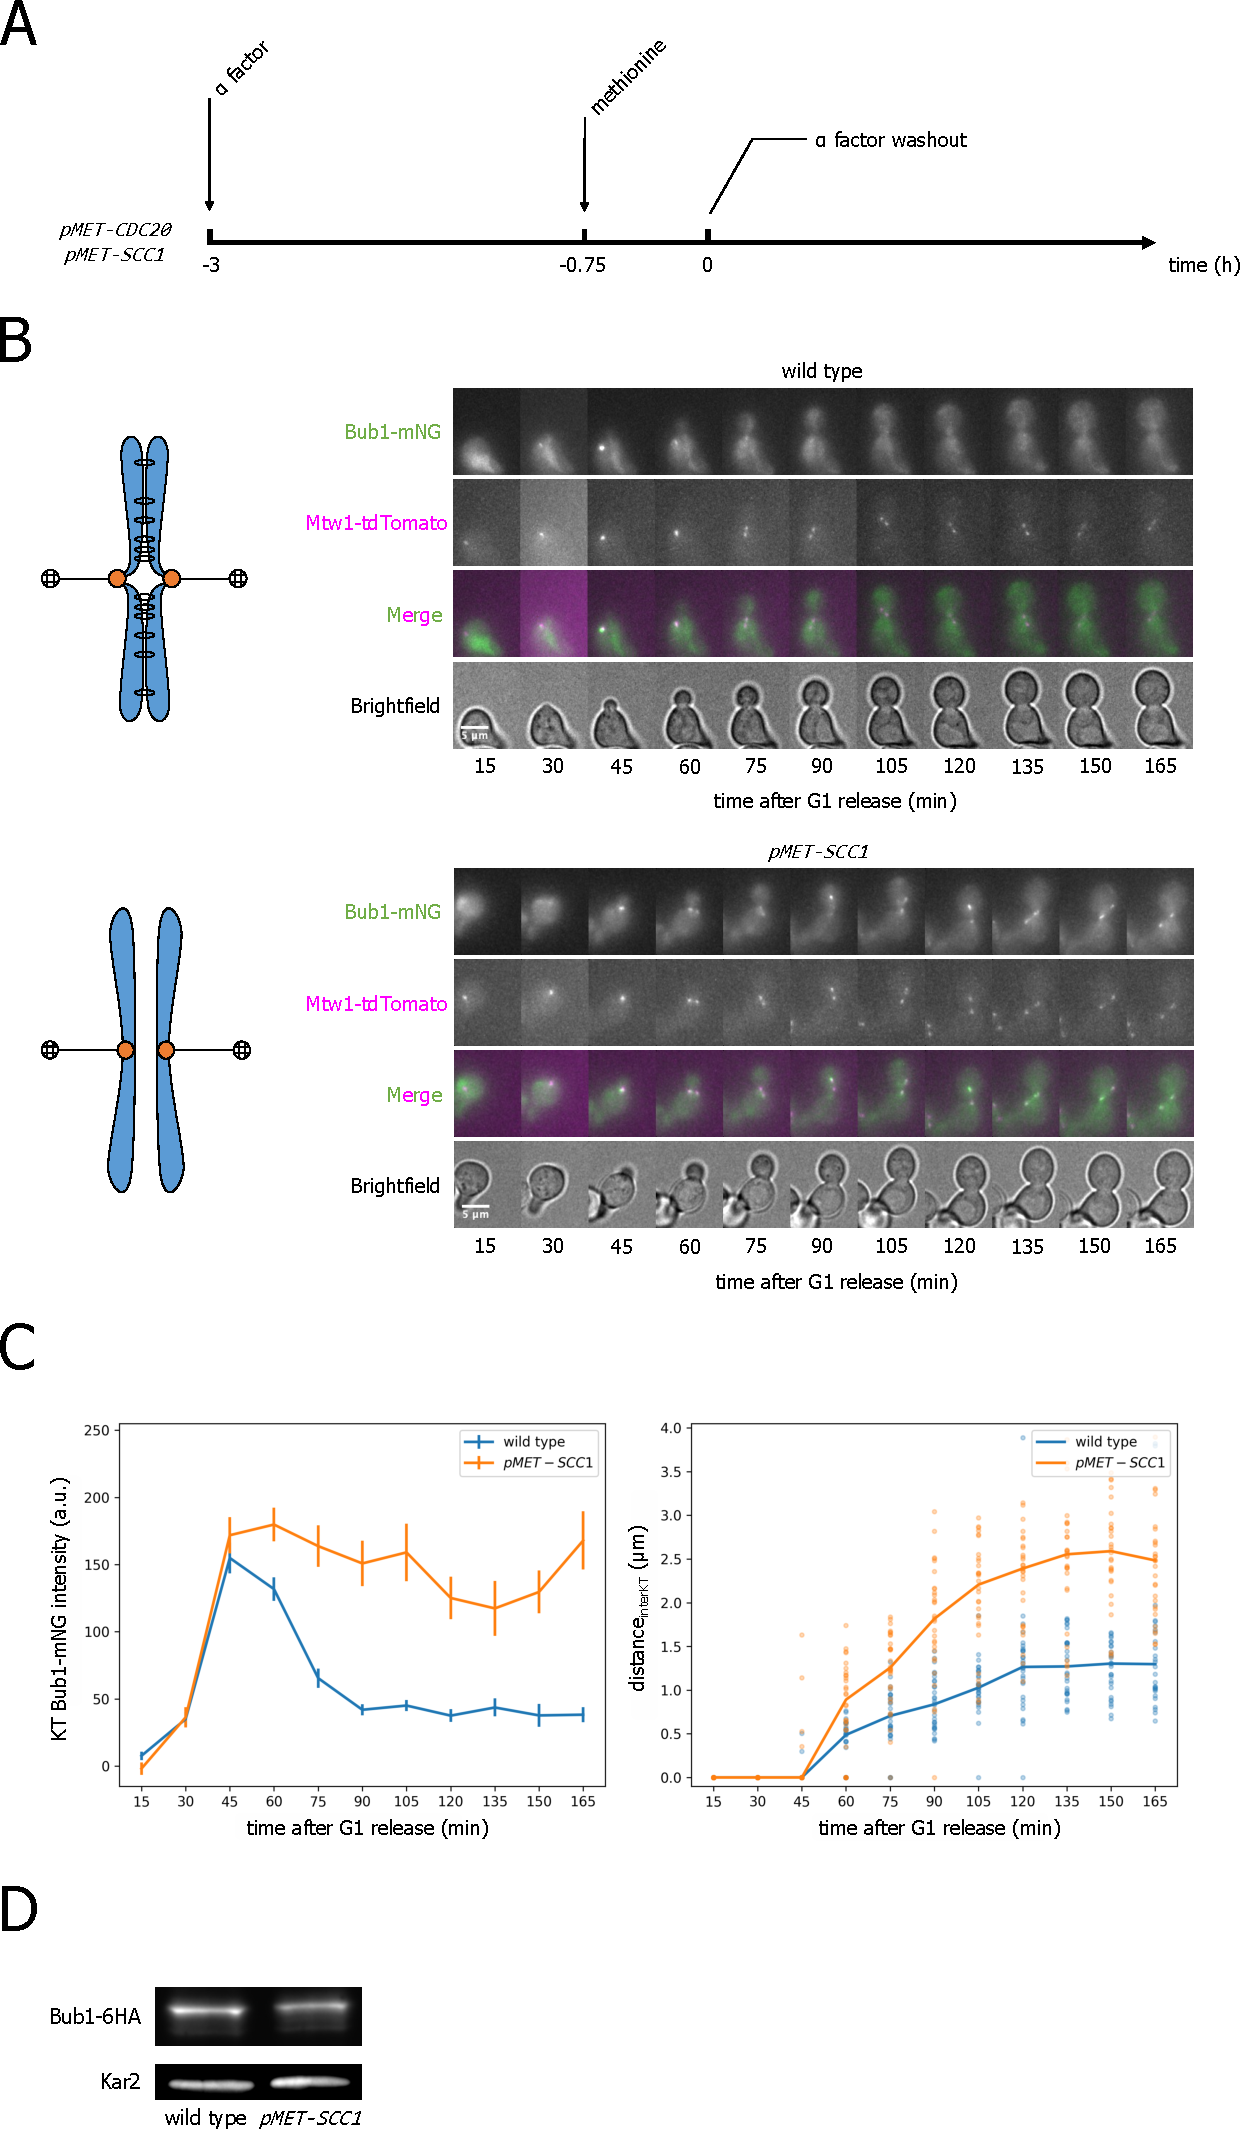
\includegraphics[width=0.9\textwidth]{chapter3/figures/Bub1-mNG pMET-SCC1.pdf}
  \caption[Tension is required for Bub1 re-localisation from the kinetochore]{Tension is required for Bub1 re-localisation from the kinetochore. (A) Schematics of experimental procedures. (B) Montage of representative time-lapse imaging. Cartoons on the left indicate the status of sister chromatids. (C) N=30 cells for each strain were followed over time and quantified for kinetochore Bub1-mNG fluorescence intensity and inter-kinetochore distance. Left panel: mean fluorescence intensity of Bub1-mNG at the kinetochore as a function of time. The error bar represents the standard error. Right panel: Median inter-kinetochore distance as a function of time. Individual data points are shown as dots. The wild type is shown in blue and \textit{pMET-SCC1} is shown in orange. (D) Western blotting with anti-HA antibody to detect Bub1 protein. Kar2 was used as the loading control. }
  \label{fig:bub1metscc1}
\end{figure} 

\subsection{Bub1 removal is sufficient for rapid de-localisation of Sgo1}
\cite{Nerusheva2014} have shown with ChIP-qPCR that Bub1 depletion abolishes Sgo1 localisation at the peri-centromere in the absence of tension, suggesting Bub1 removal triggers Sgo1 de-localisation. However, the 1 \si{\hour} time resolution of the experiment was not fine enough to explain the fast kinetics of Sgo1 re-localisation, where the transition from focused to diffused signal happens within 15 \si{\minute}. To repeat this result with an independent method as well as to improve the time resolution, I sought to repeat this experiment with microscopy. \textit{SGO1-EGFP MTW1-tdTomato pMET-CDC20} strain with additional AID system to deplete Bub1 (\textit{BUB1-3V5-AID} P$_{ADH1}$\textit{-OsTIR1-9MYC}) was synchronised in G1 and then released into nocodazole-containing media for a metaphase arrest without tension. Since Bub1 is a component of SAC, the media also does not contain methionine to prevent anaphase onset when Bub1 is depleted. Auxin NAA was then added to induce Bub1 depletion, with imaging started immediately (Figure~\ref{fig:bub1aid}A). Consistent with previous research, nocodazole-arrested cells showed large buds and signals of 2 or 3 dots for both Sgo1-EGFP and Mtw1-tdTomato \citep{Richmond2013Slk19Attachment}. In contrast to the control where DMSO was added (-NAA), Sgo1-EGFP foci disappeared after the addition of NAA (+NAA) (Figure~\ref{fig:bub1aid}C). Survival analysis indicated that the probability for cells to have a Sgo1-EGFP dot-signal started to decrease since NAA was added, with less than 20\% at 30 \si{\minute} afterwards (Figure~\ref{fig:bub1aid}D). To verify the depletion of Bub1 as well as characterising its kinetics, I performed western blotting on time course samples of cells treated identically as in the imaging experiment. The level of Bub1 protein became largely reduced at 20 \si{\minute} and barely detectable from 30 \si{\minute} after adding NAA (Figure~\ref{fig:bub1aid}E), similar to the dynamics of Sgo1 de-localisation shown in Figure~\ref{fig:bub1aid}D. This suggests a very quick response of Sgo1 localisation to Bub1 depletion, which could explain the fast re-localisation of Sgo1 previously observed \citep{Nerusheva2014}. Therefore, it is possible that the tension-dependent re-localisation of Sgo1 results from the de-localisation of Bub1 from the kinetochore by tension. 

\nomenclature{AID}{Auxin-Inducible Degron}
\nomenclature{NAA}{Naphthalene Acetic Acid}
\nomenclature{DMSO}{DiMethyl SulfOxide}

\begin{figure}[htbp]
  \centering
  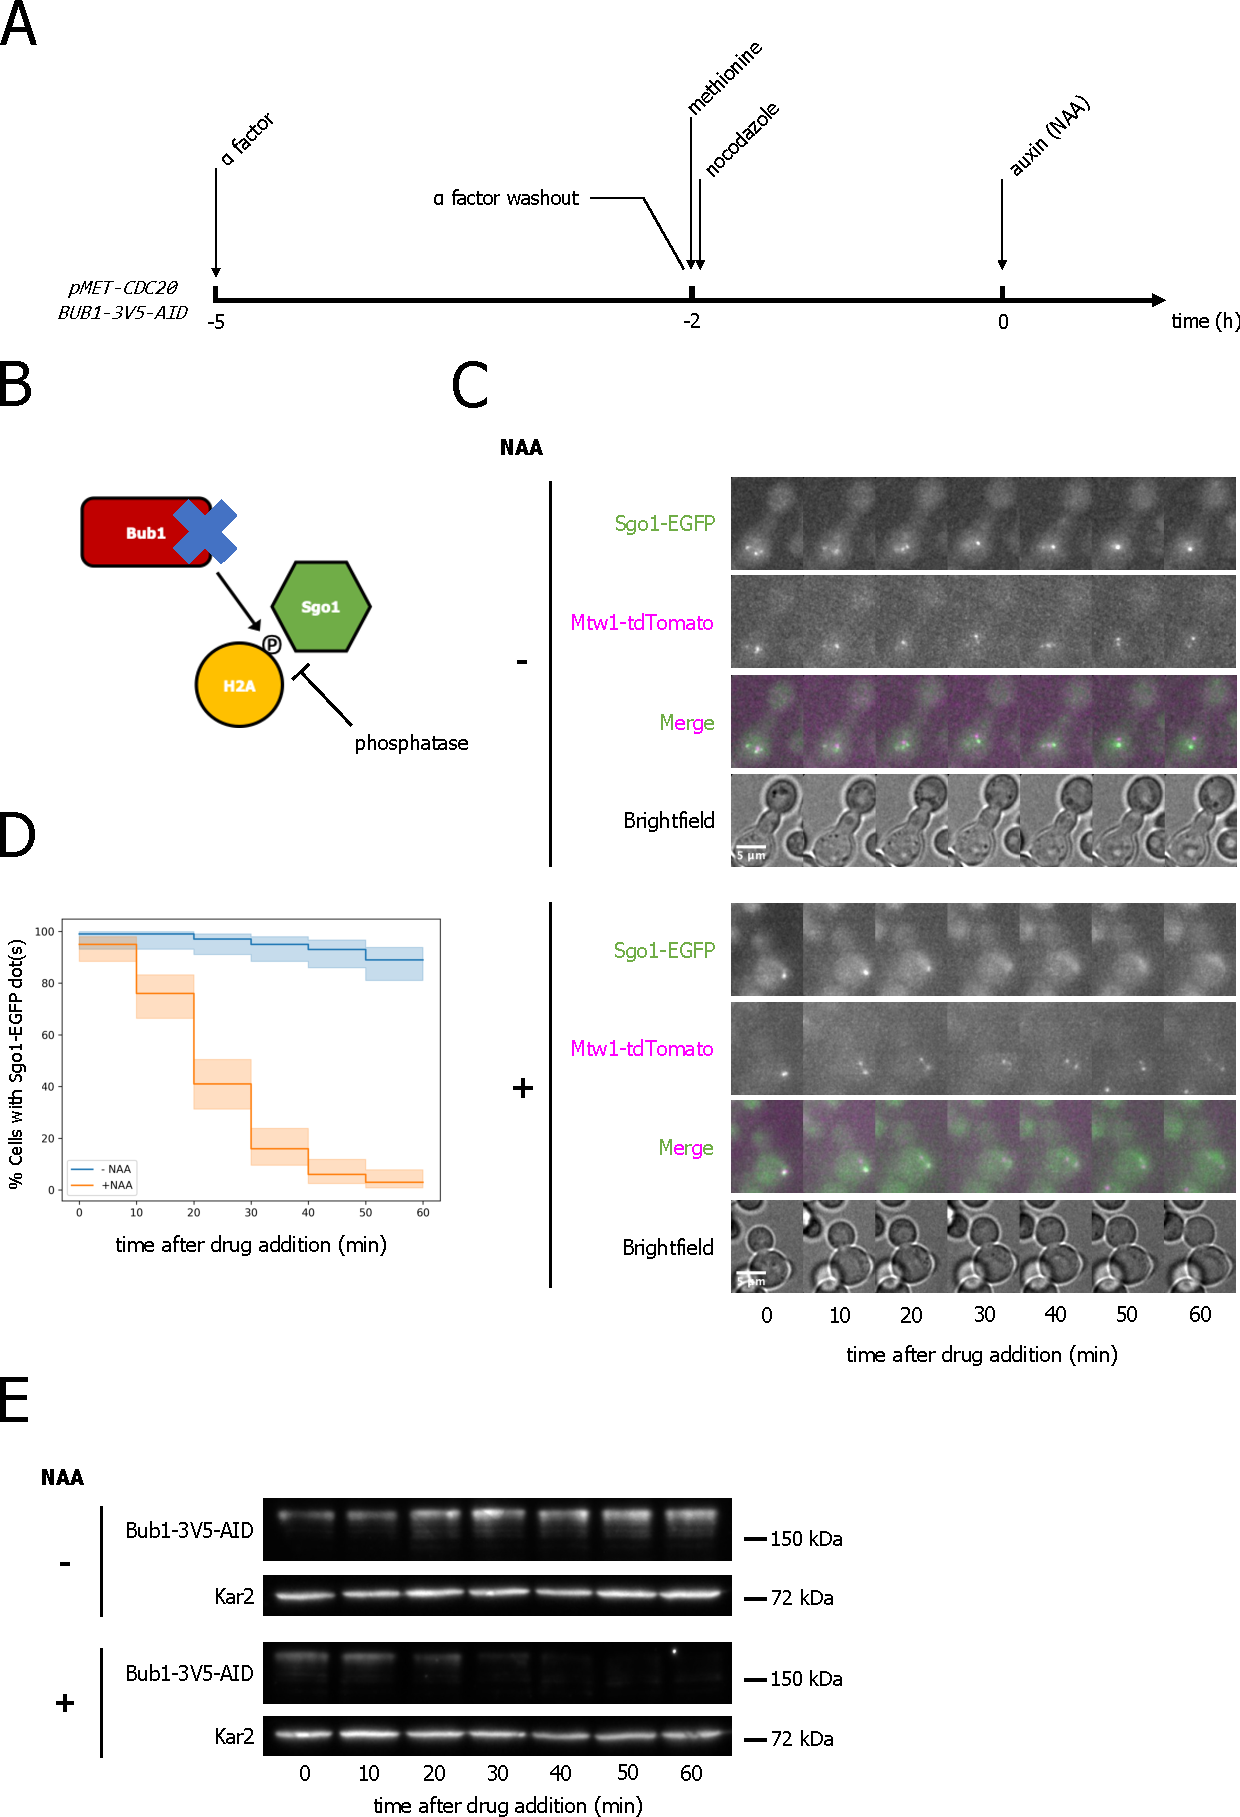
\includegraphics[width=0.9\textwidth]{chapter3/figures/Bub1-3V5-AID.pdf}
  \caption[Sgo1 is de-localised promptly upon Bub1 depletion in the absence of tension]{Sgo1 is de-localised promptly upon Bub1 depletion in the absence of tension. (A) Schematics of experimental procedures. (B) Schematics of experimental concept. (C) Montage of representative time-lapse imaging. (D) Survival analysis of the duration of focused Sgo1-EGFP signal. N=100 cells for each strain were followed over time and quantified for the duration of the Sgo1-EGFP signal being focused. Solid lines are Kaplan-Meier survival estimates. The shaded area in the same colour is the 95\% confidence limit of the estimate. (E) Western blotting with anti-V5 antibody to detect Bub1 protein. Kar2 was used as the loading control.}
  \label{fig:bub1aid}
\end{figure} 

\subsection{Bub1 re-localisation is earlier than Sgo1 re-localisation}
The data so far have suggested a model where Bub1 and Sgo1 re-localise sequentially. If this is true, there could be a difference in the timing of their re-localisation. To test it, a strain with the two proteins tagged with fluorescence proteins of different colours should be used in the ideal situation. However, none of Bub1 or Sgo1 tagged with various RFPs gave good enough signals under our microscope, possibly due to a combination of low abundance and cell-cycle-dependent expression of the two proteins. For example, Sgo1 tagged with the brightest RFP in the lab tdTomato is visible as dots in cells arrested with nocodazole but not in an unperturbed cell cycle because tdTomato has a maturation time beyond the time Sgo1 can be detected in a mitotic time course \citep{Indjeian2005a}. Instead, I could only image Bub1-mNG and Sgo1-EGFP in separate strains and use the inter-kinetochore distance measured from Mtw1-tdTomato as the internal control for timing. Standard G1 to metaphase live-cell imaging was carried out (Figure~\ref{fig:bub1sgo1}A). The inter-kinetochore distances are indistinguishable between the two strains (Figure~\ref{fig:bub1sgo1}B), suggesting a similar progress of tension establishment. Kinetochore Bub1-mNG fluorescence intensity was quantified as in the previous experiments. Due to the fact that Sgo1-EGFP is close to but does not co-localise with the kinetochore, it was not able to define the ROI to quantify fluorescence intensity. Therefore, Sgo1-EGFP was only scored for whether the signal can be counted as focused or not. Consistent with the speculation, the dynamics of Sgo1-EGFP and Bub1-mNG were similar except for a 15 \si{\minute} delay of Sgo1-EGFP in both the increase and decrease (Figure~\ref{fig:bub1sgo1}B), supporting the idea that Bub1 removal from the kinetochore triggers the de-localisation of Sgo1. 

\nomenclature{ROI}{Region Of Interest}

\begin{figure}[htbp]
  \centering
  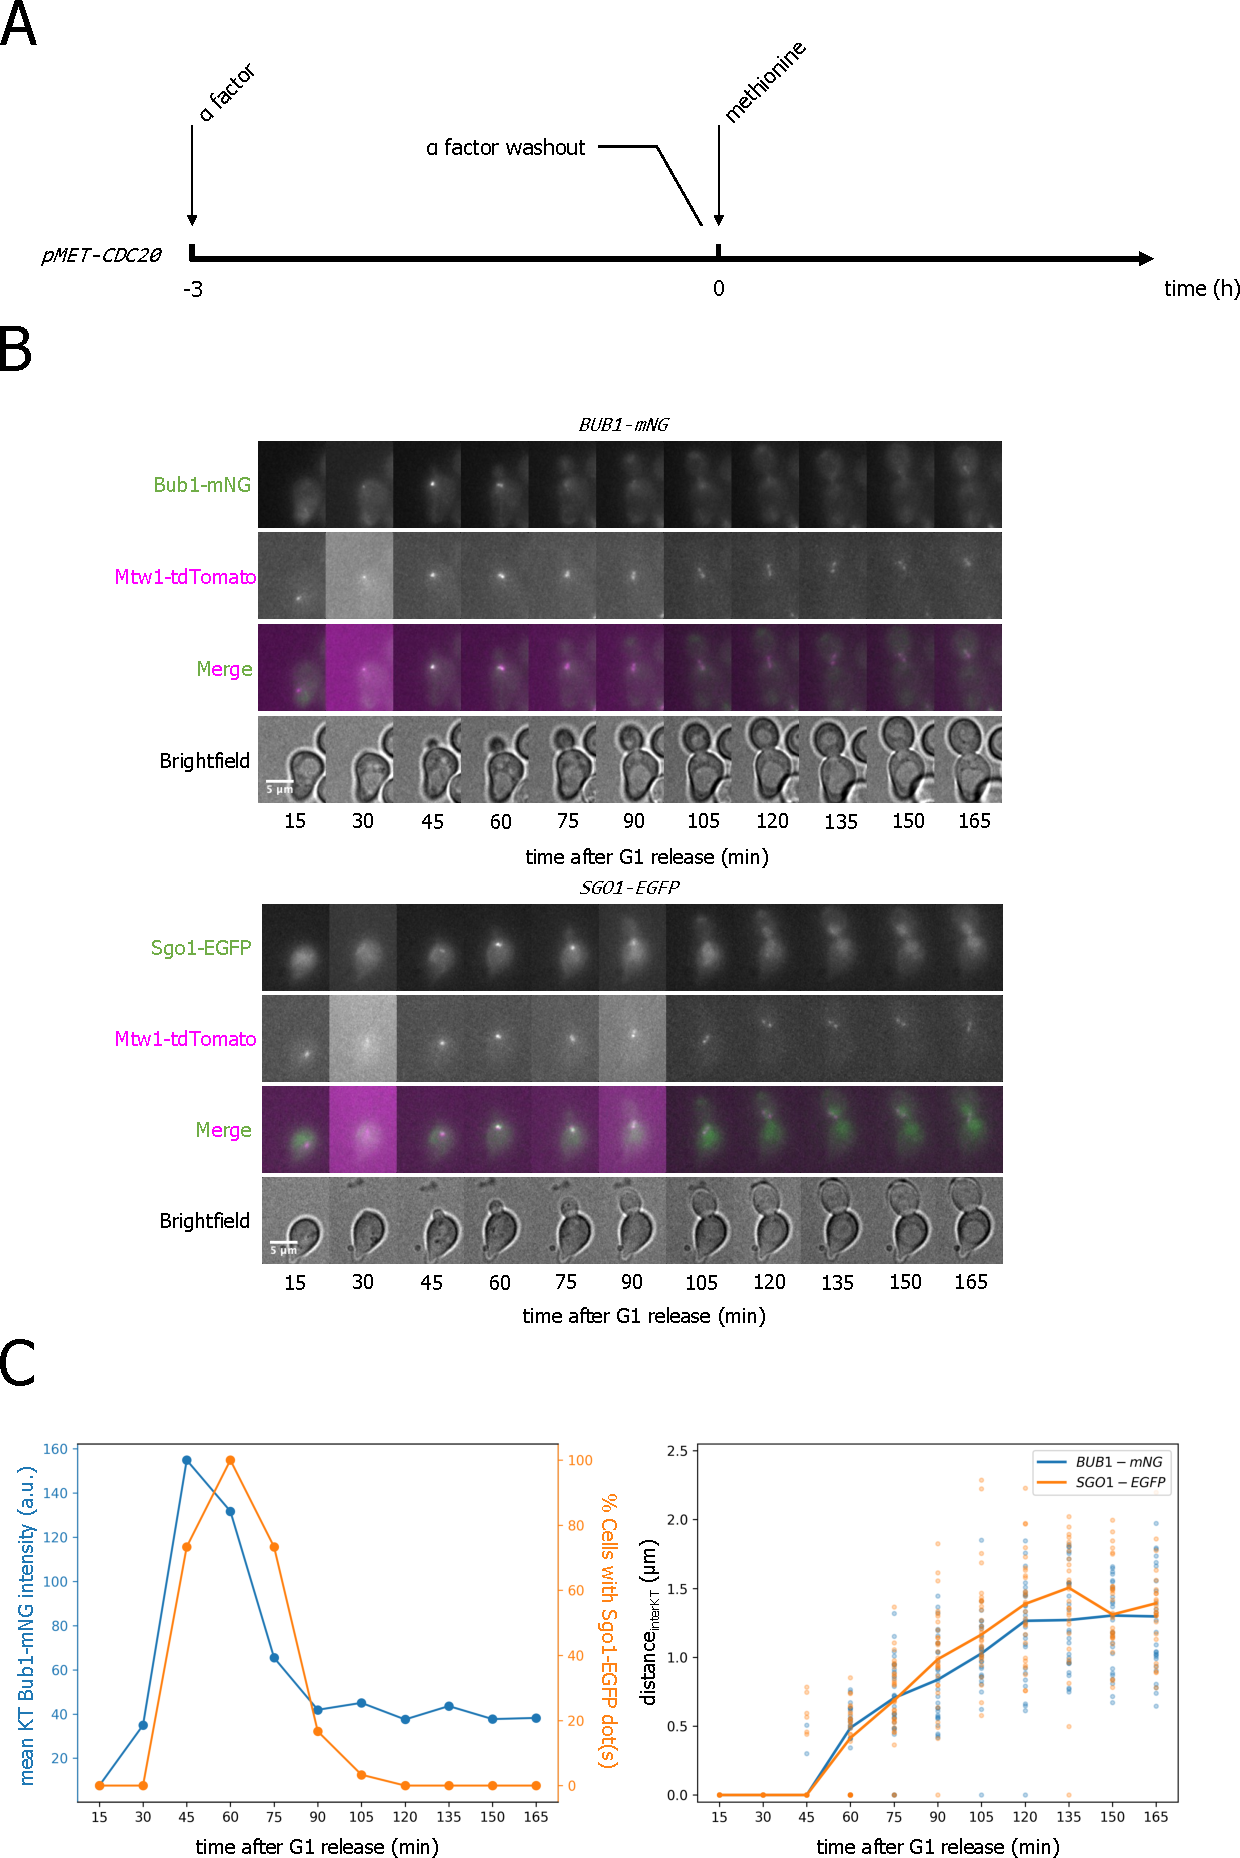
\includegraphics[width=0.9\textwidth]{chapter3/figures/Bub1-mNG Sgo1-EGFP.pdf}
  \caption[Bub1 is re-localised earlier than Sgo1]{Bub1 is re-localised earlier than Sgo1. (A) Montage of representative time-lapse imaging. (B) N=30 cells for each strain were followed over time and quantified. Left panel: mean fluorescence intensity of Bub1-mNG at the kinetochore and percentage of cells with Sgo1 foci as a function of time. Right panel: Median inter-kinetochore distance as a function of time. Individual data points are shown as dots. The \textit{BUB1-mNG} strain is shown in blue and the \textit{SGO1-EGFP} strain is shown in orange.}
  \label{fig:bub1sgo1}
\end{figure} 

\subsection{The continued presence of Bub1 is required to maintain H2A-pS121}
Our naive model argues that the phosphorylation status of the key substrate(s) determining Sgo1 localisation should be regulated by the kinase-phosphatase balance between Bub1 and unknown phosphatase(s) (Figure~\ref{fig:naive}). Therefore, the substrate(s) is expected to be phosphorylated in the absence of tension and de-phosphorylated when existing Bub1 is depleted as in the previous experiment (Figure~\ref{fig:ph2abub1aid}B). Given the demonstrated role of H2A-pS121 in localising Sgo1 to the peri-centromere \citep{Kawashima2010a, Fernius2007Bub1Mitosis, Nerusheva2014}, I hypothesised that it is the key Bub1 substrate being regulated. To directly monitor the phosphorylation status of H2A-S121, I ordered phospho-specific antibodies from Genscript. Western blotting using these antibodies indicated that they are able to distinguish phosphorylated H2A-S121 from unphosphorylated one as there is a less-than-17-\si{\kilo\dalton} band bright in wild type but extremely dim in Bub1 kinase-dead mutant (\textit{bub1$\Delta$K}) or H2A phospho-null mutant (H2A-S121A) arrested by nocodazole (Figure~\ref{fig:abtest}). 

\begin{figure}[htbp]
  \centering
  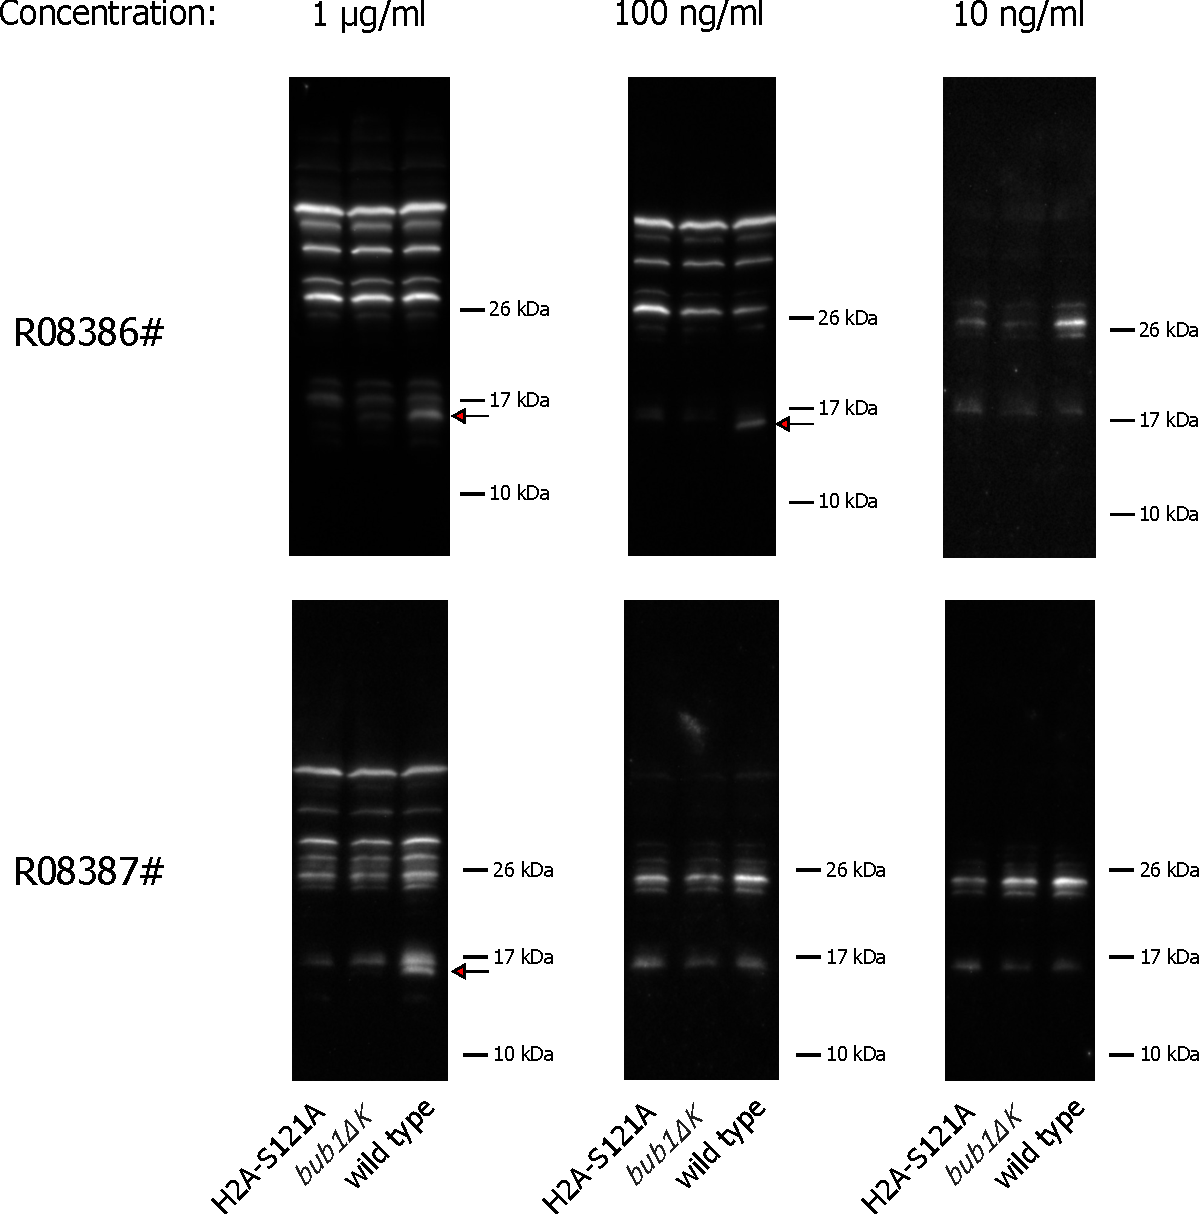
\includegraphics[width=0.9\textwidth]{chapter3/figures/pH2A ab test.pdf}
  \caption[Validation of phospho-specific antibodies for H2A-pS121]{Validation of phospho-specific antibodies for H2A-pS121. Western blotting on H2A-S121A, \textit{bub1$\Delta$K} or wild type arrested by nocodazole using anti-Hta2-pS122 antibodies generated from host R08386\# or R08387\# (GenScript) at 1 \si{\micro\gram/\milli\litre}, 100 \si{\nano\gram/\milli\litre} or 10 \si{\nano\gram/\micro\litre}. Red arrows indicate the specific bands. }
  \label{fig:abtest}
\end{figure} 

To test whether H2A is indeed de-phosphorylated at S121 upon Bub1 depletion, I conducted western blotting on samples from the experiment of Figure~\ref{fig:bub1aid} (Figure~\ref{fig:ph2abub1aid}A). The specific band is maintained within the scope of the experiment in -NAA samples. In contrast, it is reduced in +NAA samples in spite of the increase in the intensity of the non-specific band above (Figure~\ref{fig:ph2abub1aid}C), suggesting that H2A-pS121 is being de-phosphorylated due to Bub1 depletion. Hence, the continued presence of Bub1 is required to maintain H2A-pS121, favouring the naive model and the idea that H2A-pS121 is the key substrate. Due to the non-ideal specificity of the antibody over unphosphorylated H2A-S121, it is difficult to interpret the kinetics of the de-phosphorylation. 

\begin{figure}[htbp]
  \centering
  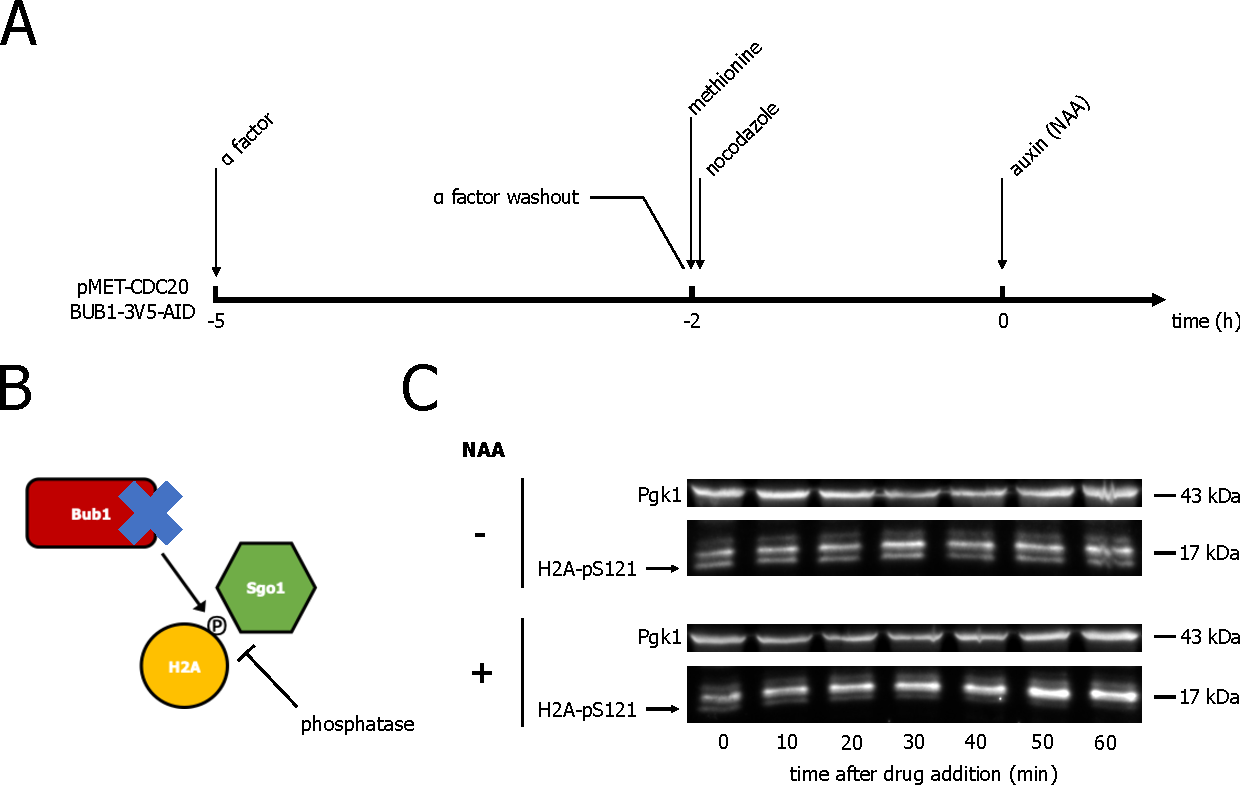
\includegraphics[width=0.9\textwidth]{chapter3/figures/pH2A Bub1-AID.pdf}
  \caption[Bub1 depletion leads to a reduction in H2A-S121 phosphorylation in the absence of tension]{Bub1 depletion leads to a reduction in H2A-S121 phosphorylation in the absence of tension. (A) Schematics of experimental procedures. (B) Schematics of experimental concept. (C) Western blotting with anti-H2A-pS121 antibody to detect the phosphorylation status of H2A. Pgk1 was used as the loading control.}
  \label{fig:ph2abub1aid}
\end{figure} 

\subsection{Total cellular H2A-pS121 level is independent of tension}
\label{subsec:totalph2aindten}

Since tension de-localises Bub1 from the kinetochore, physically separating it from its substrate H2A at the peri-centromere, I hypothesised that the phosphorylation of H2A-S121 would be lost or at least reduced by tension. Therefore, I arrested wild type strain, the control strain used for imaging and the negative control \textit{bub1$\Delta$K} in the presence or absence of tension (Figure~\ref{fig:ph2atension}A). Western blotting against H2A-pS121 was conducted as before. Surprisingly, tension did not decrease the intensity of the specific band for both wild type and the imaging strain (Figure~\ref{fig:ph2atension}B), indicating the level of total cellular H2A-pS121 is independent of tension. It seems that tension even increased the specific band intensity for the imaging strain. However, I believe it is due to the variation in the blotting process, as the intensity of the non-specific band is also reduced in the no tension sample compared to the tension sample. 

\begin{figure}[htbp]
  \centering
  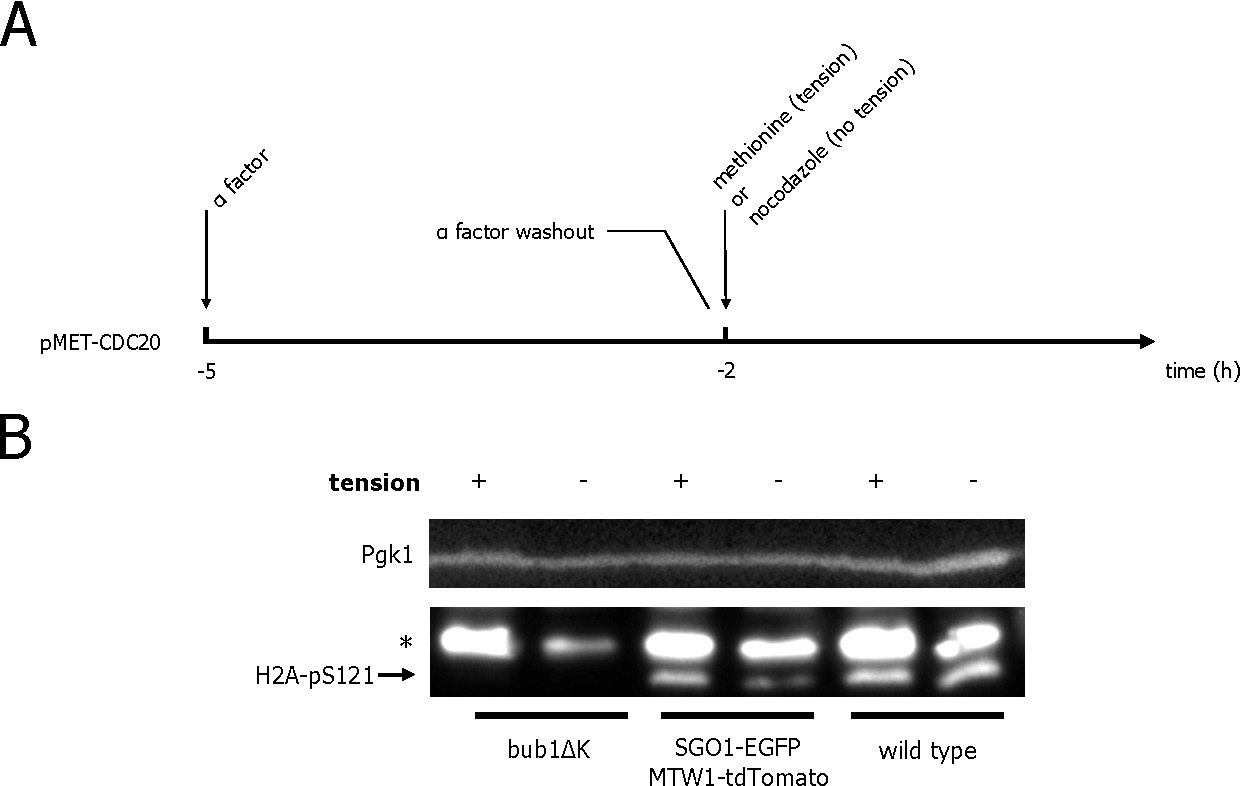
\includegraphics[width=0.9\textwidth]{chapter3/figures/pH2A tension.pdf}
  \caption[Total cellular H2A-pS121 level is independent of tension]{Total cellular H2A-pS121 level is independent of tension.(A) Schematics of experimental procedures. (B) Western blotting with anti-H2A-pS121 antibody to detect the phosphorylation status of H2A. Pgk1 was used as the loading control. The asterisk represents the non-specific band.}
  \label{fig:ph2atension}
\end{figure}

To validate this unexpected result, I turned to a different approach where H2A-pS121 were monitored over the entire cell cycle. Cells bearing \textit{PDS1-HA} were synchronised in G1 and released into rich media as described in the previous synchronised mitotic time course experiment (Figure~\ref{fig:ph2atimecourse}A). Tubulin IF indicated that most cells were in metaphase at 75 \si{\minute} after G1 release while in anaphase at 90 and 105 \si{\minute} (Figure~\ref{fig:ph2atimecourse}B). Western blotting with anti-HA and anti-H2A-pS121 was then performed on the time course samples. The securin Pds1 peaked at 75 \si{\minute} and became barely visible at 90 \si{\minute}, consistent with the cell cycle stages information from the tubulin IF. The H2A-pS121 band was comparable from 60 to 90 \si{\minute}, with a sharp reduction at 105 \si{\minute}, suggesting the level of H2A-pS121 is maintained during the metaphase-anaphase transition, therefore verifying the previous result. The reason that the non-specific bands here appeared differently from the previous experiments is likely due to the fact that I used a large protein gel in this western blotting for better protein resolution. Interestingly, the dynamics of H2A-pS121 level over the cell cycle are qualitatively similar to that of Bub1 protein level (Figure~\ref{fig:bub1timecourse}). 

\begin{figure}[htbp]
  \centering
  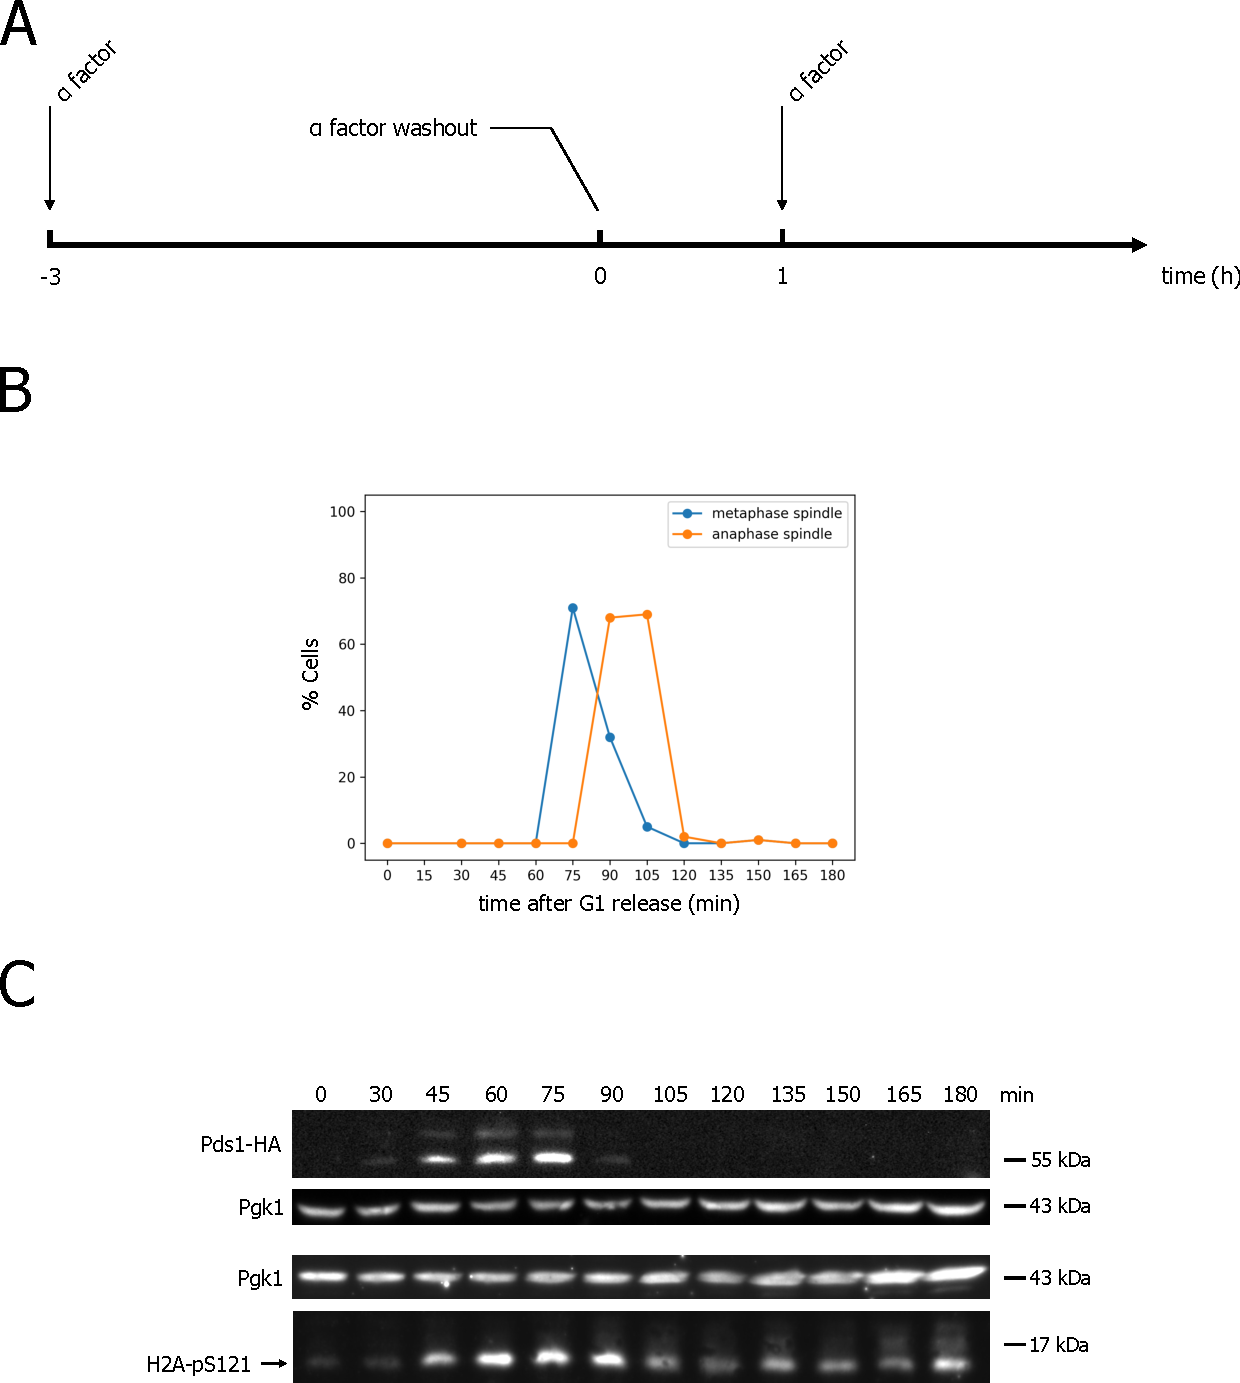
\includegraphics[width=0.9\textwidth]{chapter3/figures/pH2A mitotic time course.pdf}
  \caption[H2A-pS121 level is maintained during metaphase-anaphase transition]{H2A-pS121 level is maintained during metaphase-anaphase transition. (A) Schematics of experimental procedures. (B) The proportion of cells with metaphase or anaphase spindle over time by tubulin IF. (C) Upper: western blotting with anti-HA antibody to detect Pds1 protein. Pgk1 was used as the loading control. Lower: western blotting with anti-H2A-pS121 antibody to detect the phosphorylation status of H2A. Pgk1 was used as the loading control.}
  \label{fig:ph2atimecourse}
\end{figure}

\subsection{Tension re-distributes H2A-pS121 from the centromere to the chromosome arm}

Intuitively, the total level of H2A-pS121 being unaffected by tension contradicts the previous finding that its maintenance requires continued Bub1 and Bub1 is de-localised from the kinetochore upon tension. However, one possibility that can explain both is that de-localised Bub1 reaches and phosphorylates H2A molecules other than the ones localised at the peri-centromere whereas the previously phosphorylated ones at the peri-centromere started to be de-phosphorylated, resulting in a change in the localisation of H2A-pS121 but not the total level. To test this hypothesis, we sought to conduct either IF or ChIP using the H2A-pS121 phospho-specific antibody. Considering the poor specificity of the antibody, I turned to ChIP because it is supposed to provide a better signal-to-noise ratio. 

First, I carried out a test ChIP-qPCR to determine whether the antibody can be used for ChIP as well as the optimal fixing time. Tensionless metaphase wild type or \textit{bub1$\Delta$K}, the negative control, cells arrested by nocodazole were fixed for 10, 20, 30 and 60 \si{\minute}. Samples were then subject to ChIP with the anti-H2A-pS121 antibody and qPCR was used to determine the enrichment at the centromere, chromosome arm and peri-centromere of chromosome IV. Signals were detected at the centromere and peri-centromere in wild type but not in \textit{bub1$\Delta$K}, showing that the antibody is capable of ChIP application. Consistent with the localisation in vertebrates by IF experiments \citep{Ricke2012, Kawashima2010a, Liu2013a, Williams2017Bub1Kinetochores, Zhang2020FunctioningMitosis, Liang2019ACells, Lee2008, Liu2015}, H2A-pS121 enrichment is vastly reduced on the chromosome arm in wild type. The fixing time does not seem to be important for this particular experiment. I decided to use 10 \si{\minute} as it should cross-link fewer irrelevant proteins to the DNA in theory and therefore reduce the likelihood of potential artefacts. 

\begin{figure}[htbp]
  \centering
  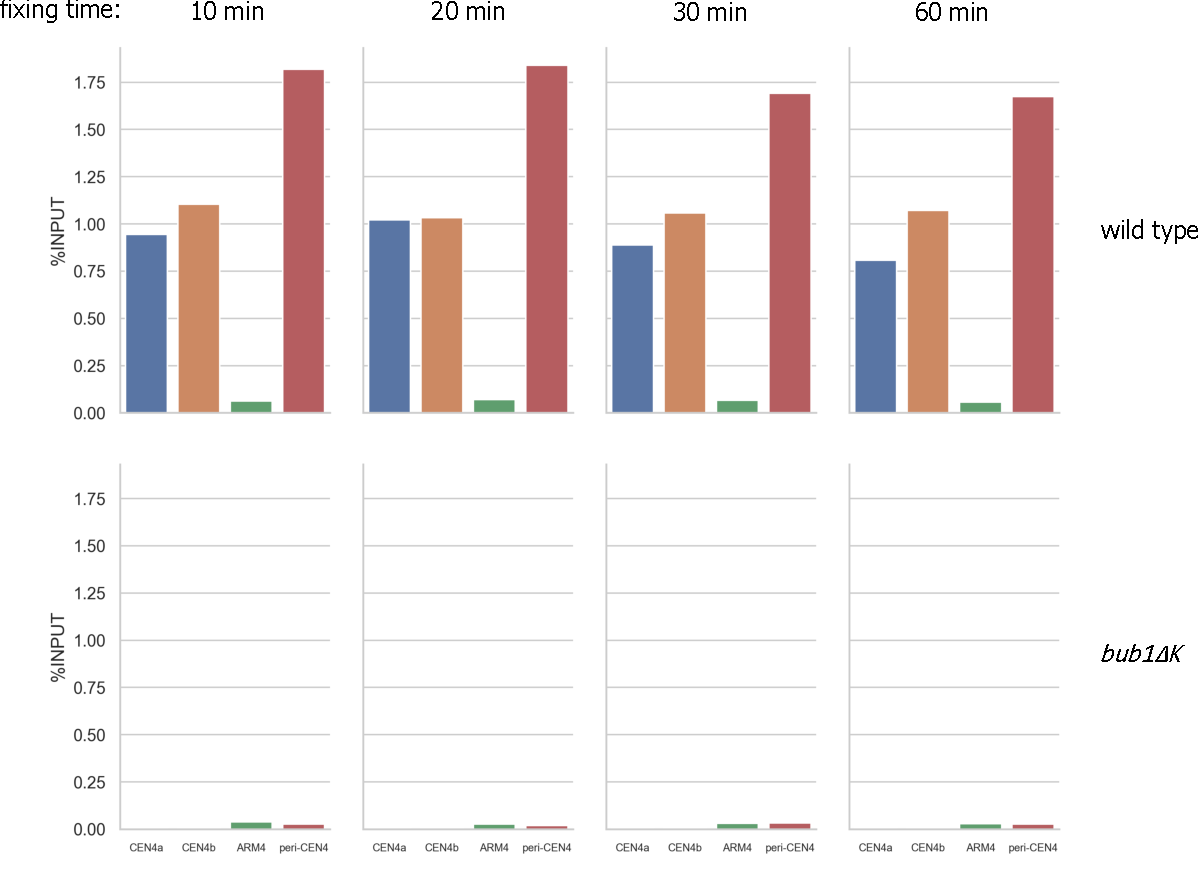
\includegraphics[width=0.9\textwidth]{chapter3/figures/pH2A test ChIP-qPCR.pdf}
  \caption[The H2A-pS121 phospho-specific antibody can be used for ChIP]{The H2A-pS121 phospho-specific antibody can be used for ChIP. Wild type and \textit{bub1$\Delta$K} cells arrested in metaphase without tension were fixed for 10, 20, 30 and 60 minutes, respectively, and subjected to H2A-pS121 ChIP-qPCR at 4 different loci, with two at the centromere, one at chromosome arm and one at the peri-centromere of chromosome IV. }
  \label{fig:ph2atestchipqpcr}
\end{figure}

Next, I conducted a formal H2A-pS121 ChIP-seq experiment. To be able to compare signals between samples, a wet calibration method was used, where the genome from another species, fission yeast in this case, was mixed with the budding yeast genome in the experiment \citep{Hu2015BiologicalChIP-seq}. Wild type cells were arrested in metaphase with or without tension (Figure~\ref{fig:ph2achipseqchecking}A). Tubulin IF indicated that they have good synchronisation. 98\% cells from the tension sample displayed metaphase spindle while none of the cells from the no tension sample showed a spindle (Figure~\ref{fig:ph2achipseqchecking}B). Western blotting was used to examine the level of H2A-pS121 in the two samples. Consistent with the previous results (Subsection~\ref{subsec:totalph2aindten}), both samples showed comparable band intensities (Figure~\ref{fig:ph2achipseqchecking}C). ChIP-processed samples were further checked by qPCR for the enrichment of budding and fission yeast's loci to ensure quality. Similar to the test qPCR, the no tension sample showed high signals at the centromere and peri-centromere but not on the chromosome arm. Consistent with the idea that tension might affect the localisation of H2A-pS121, the tension sample had low signals at all three loci (Figure~\ref{fig:ph2achipseqchecking}D). The amount of fission yeast cells used for calibration is the same between samples. Therefore, it is expected that both of them should give equal enrichment at a given locus. Indeed, the signals were comparable between samples at the centromere core and outer repeat of fission yeast (Figure~\ref{fig:ph2achipseqchecking}E). 

\begin{figure}[htbp]
  \centering
  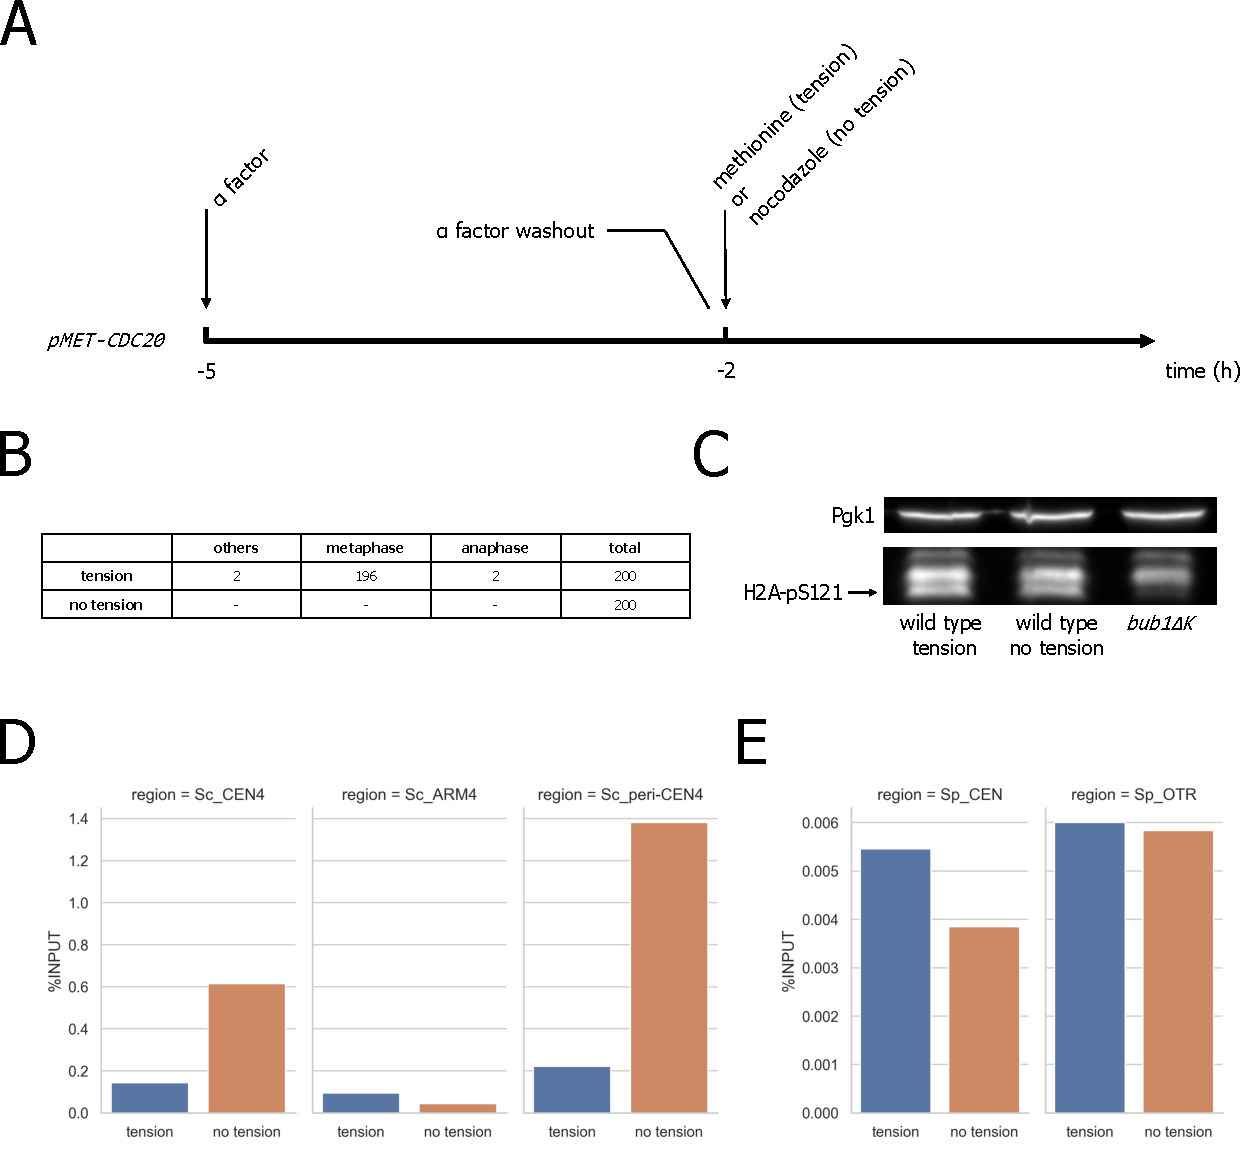
\includegraphics[width=0.9\textwidth]{chapter3/figures/checking.pdf}
  \caption[Quality control of calibrated H2A-pS121 ChIP-seq]{Quality control of calibrated H2A-pS121 ChIP-seq. (A) Schematics of experimental procedures. (B) Spindle morphology count by tubulin IF. (C) Western blotting with anti-H2A-pS121 antibody to detect the phosphorylation status of H2A. Pgk1 was used as the loading control. (D) H2A-pS121 ChIP-qPCR at the chromosome IV centromere, chromosome arm and peri-centromere of \textit{S.cerevisiae}. (E) H2A-pS121 ChIP-qPCR at chromosome I centromere core and outer repeat of \textit{S.pombe}. }
  \label{fig:ph2achipseqchecking}
\end{figure}

With quality control conducted, I proceeded with the ChIP samples and set up sequencing. The enrichment profile of a representative chromosome, chromosome IV, is shown in Figure~\ref{fig:ph2achipseq2nd}A. H2A-pS121 has a bell-shaped distribution at the centromere in both the tension and no tension sample. However, quantitatively, consistent with the result from qPCR, the signals were massively reduced in the tension sample. In contrast, on the chromosome arm, the signals were higher for the tension sample, supporting the hypothesis. This is confirmed by piling up all 16 chromosomes. At centromeres, the signals of the tension sample were about a quarter of that of the no tension sample, whereas, on the arms, the former showed a roughly one-fold increase from the latter (Figure~\ref{fig:ph2achipseq2nd}B). To provide a more quantitative view, I categorised sequencing reads as either at centromeres or on the chromosome arms. Although the total number was similar, only 18\% of reads were assigned to the centromeres in the tension sample while the number is 63\% in the no tension sample (Figure~\ref{fig:ph2achipseq2nd}C). Hence, we concluded that the establishment of tension caused a re-distribution of H2A-pS121 from the centromere to the chromosome arm. 

\begin{figure}[htbp]
  \centering
  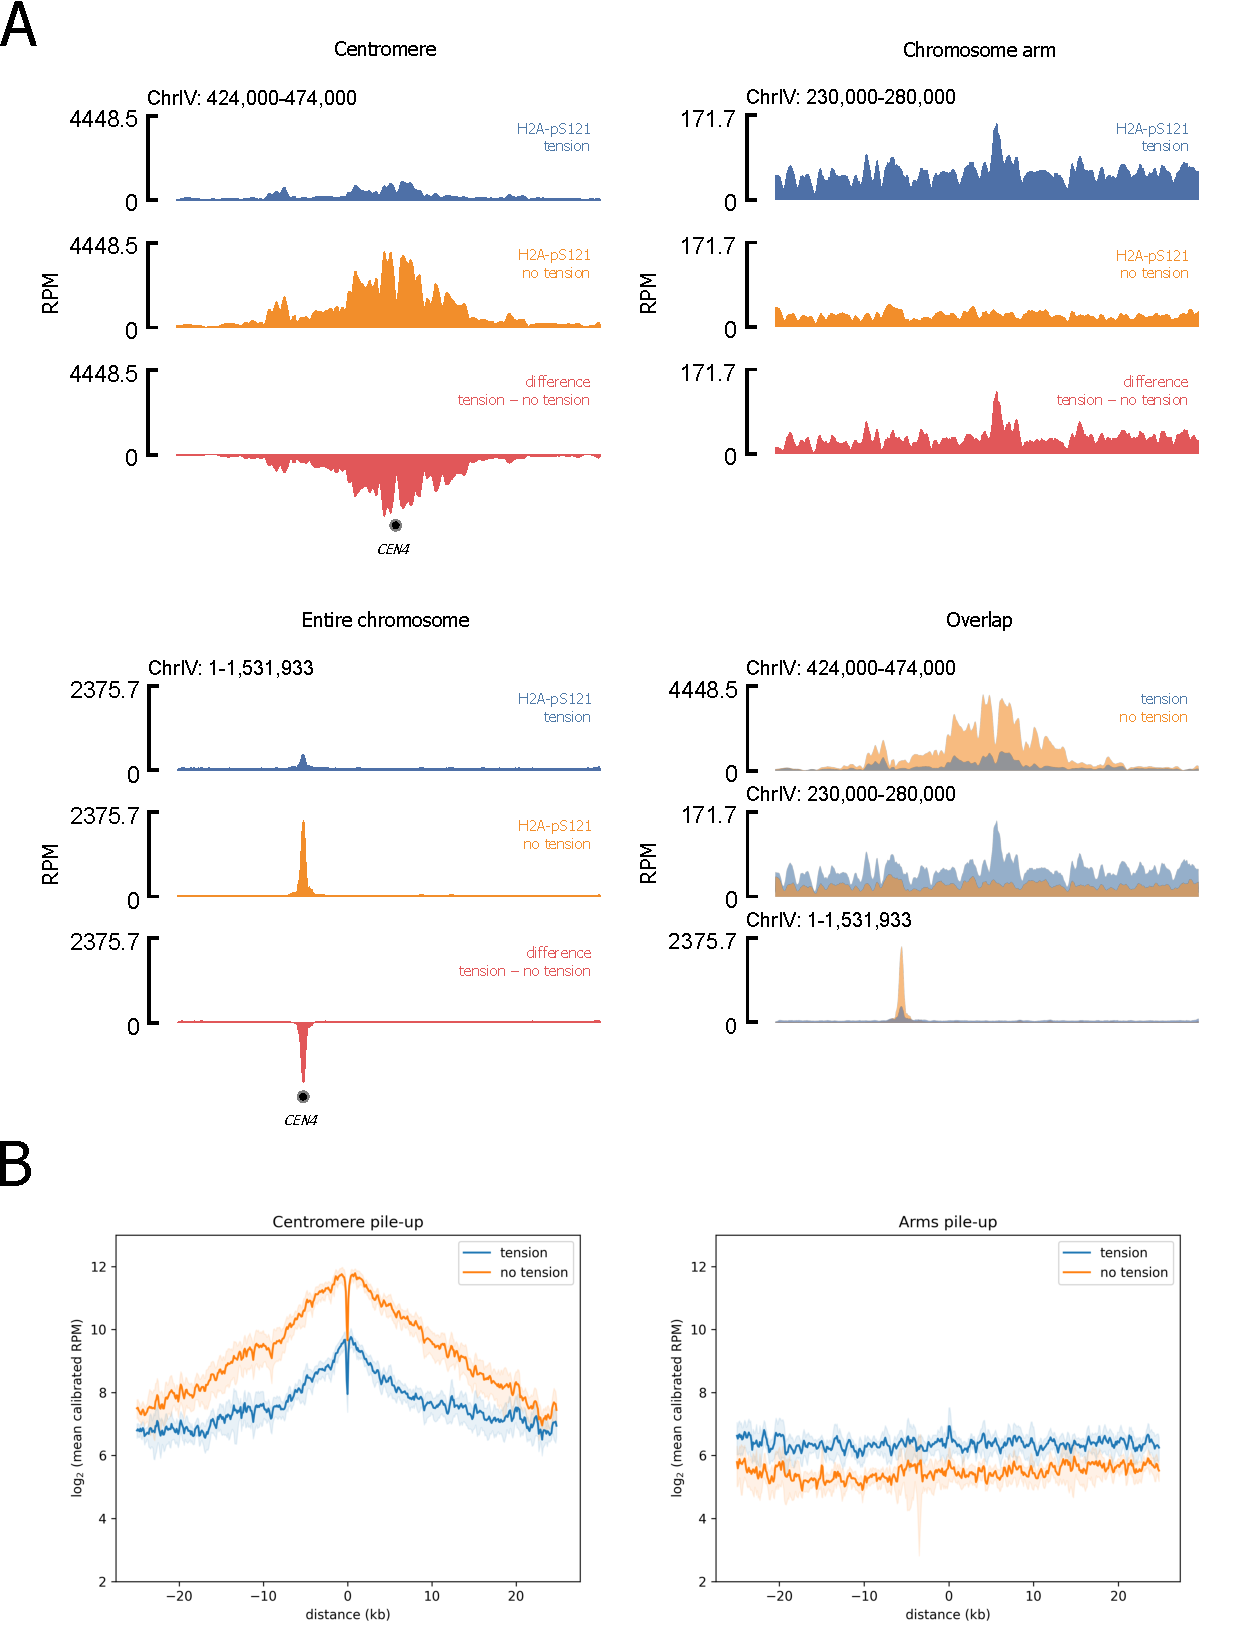
\includegraphics[width=0.9\textwidth]{chapter3/figures/pH2A ChIP-seq_1st.pdf}
\end{figure}

\begin{figure}[t]
  \centering
  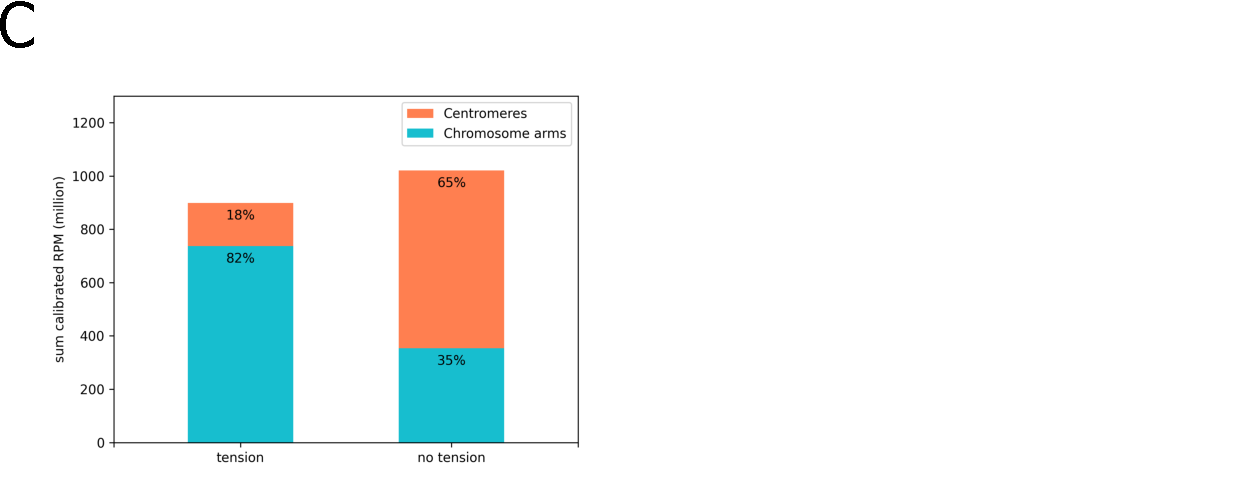
\includegraphics[width=0.9\textwidth]{chapter3/figures/pH2A ChIP-seq_2nd.pdf}
  \caption[H2A-pS121 is re-distributed from centromere to chromosome arm upon the establishment of tension]{H2A-pS121 is re-distributed from centromere to chromosome arm upon the establishment of tension. (A) Calibrated H2A-pS121 ChIP-seq profiles of cells arrested in metaphase with or without tension and their difference (tension - no tension) at the 50kb region around the centromere of chromosome IV (upper left), a 50kb region on the left arm of chromosome IV (upper right) and the entire chromosome IV (bottom left). The overlapped profiles are shown in the bottom right. (B) Pile-up of centromeres and chromosome arms. Left: the 50kb regions around the centromeres of all 16 chromosomes. Right: the 50kb regions around chromosome arms (80kb left to the centromere) of all 16 chromosomes. (C) The number of sequencing reads assigned to centromeres (the 50kb-region flanking the core centromere) or chromosome arms in each sample. }
  \label{fig:ph2achipseq2nd}
\end{figure}

\subsection{Sgo1 cannot be concentrated at the peri-centromere in H2A phospho-mimic mutant}

The re-distribution of H2A-pS121 upon tension points to a possibility that it triggers Sgo1 re-localisation. If it is true, The H2A phospho-mimic mutant whose mark for Sgo1 localisation spreads along the entire chromosome, and thus mimicking the tension situation, should lose its Sgo1 enrichment at peri-centromere in the absence of tension. However, \cite{Nerusheva2014} reported an opposite result and, combined with other results, eventually reached the conclusion that Bub1 has substrates other than H2A important for Sgo1 localisation. Due to a lack of supporting evidence from other species and the difficulty of making H2A mutants in budding yeast, I decided to verify the results by first sequencing the original strains used in the research. Surprisingly, The H2A phospho-mimic mutants turned out to be wild type for the HTA1 locus (Figure~\ref{fig:h2as121dseq}), consistent with the observation that strains with H2A-S121D mutations always show the same phenotype as wild type in the paper. 

\begin{figure}[htbp]
  \centering
  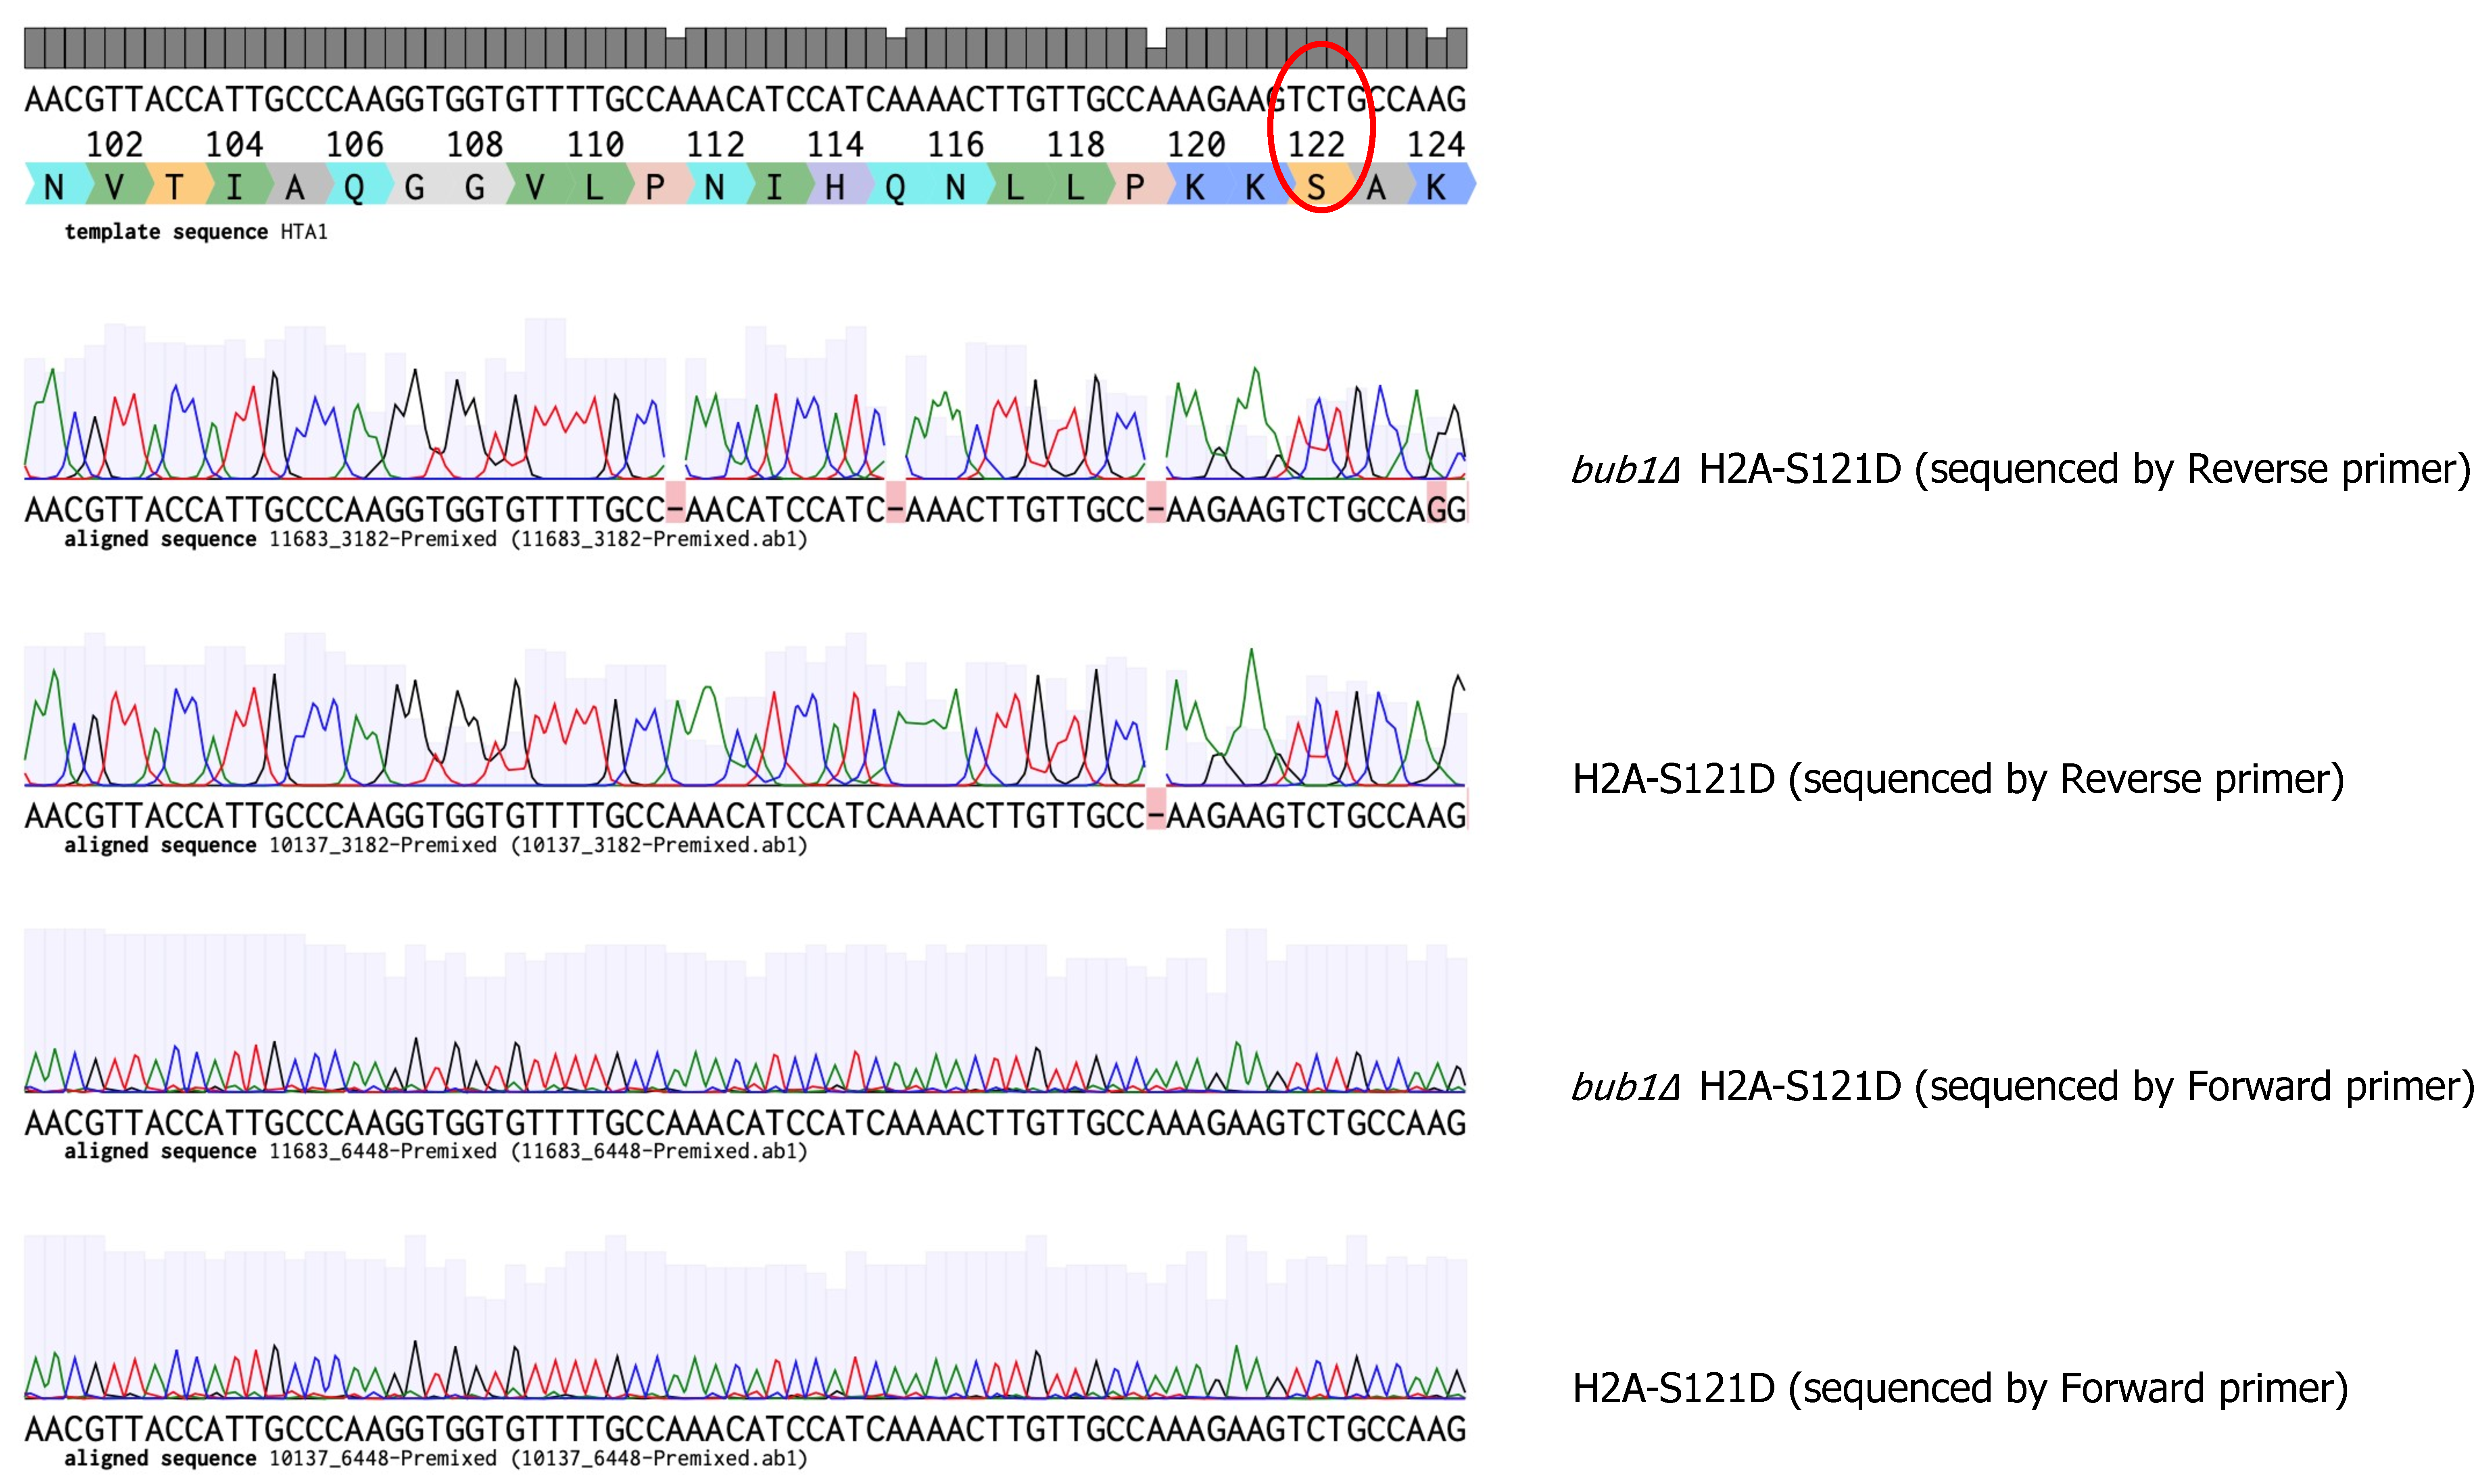
\includegraphics[width=0.9\textwidth]{chapter3/figures/nerusheva_sequencing.pdf}
  \caption[H2A phopho-mimic mutants used in \citep{Nerusheva2014} bear wild type sequence]{Phopho-mimic mutants used in \citep{Nerusheva2014} bear wild type sequence. The red circle indicates the expected mutation site.}
  \label{fig:h2as121dseq}
\end{figure}

To test whether Sgo1 localisation is altered in H2A phospho-mimic mutants, I re-constructed the strain and repeated the Sgo1-6HA ChIP-qPCR experiment by \cite{Nerusheva2014}. The standard cell harvesting procedure comparing tension with no tension conditions was performed on no tag, wild type, H2A-S121A, as a negative control, and H2A-S121D (Figure~\ref{fig:sgo1chiph2amutants}A). Tubulin IF indicated synchronised metaphase arrest in the tension samples and an absence of spindle in the no tension samples (Figure~\ref{fig:sgo1chiph2amutants}B). Western blotting showed comparable Sgo1 expression in wild type, H2A-S121A and H2A-S121D but not in no tag (Figure~\ref{fig:sgo1chiph2amutants}C). Samples then underwent ChIP processing and qPCR was used to determine the enrichment at the chromosome arm, peri-centromere and centromere of chromosome IV (Figure~\ref{fig:sgo1chiph2amutants}D). As expected, Sgo1 exhibited increased association with chromatin at the centromeric/ peri-centromeric region but not on the arm in wild type without tension. However, this increase was abolished in H2A-S121A or H2A-S121D, suggesting Sgo1 cannot be enriched at peri-centromere even in the absence of tension, supporting the idea that the phospho-mimic mutant resembles the scenario with established tension regarding Sgo1 localisation (Figure~\ref{fig:sgo1chiph2amutants}E). 

\begin{figure}[htbp]
  \centering
  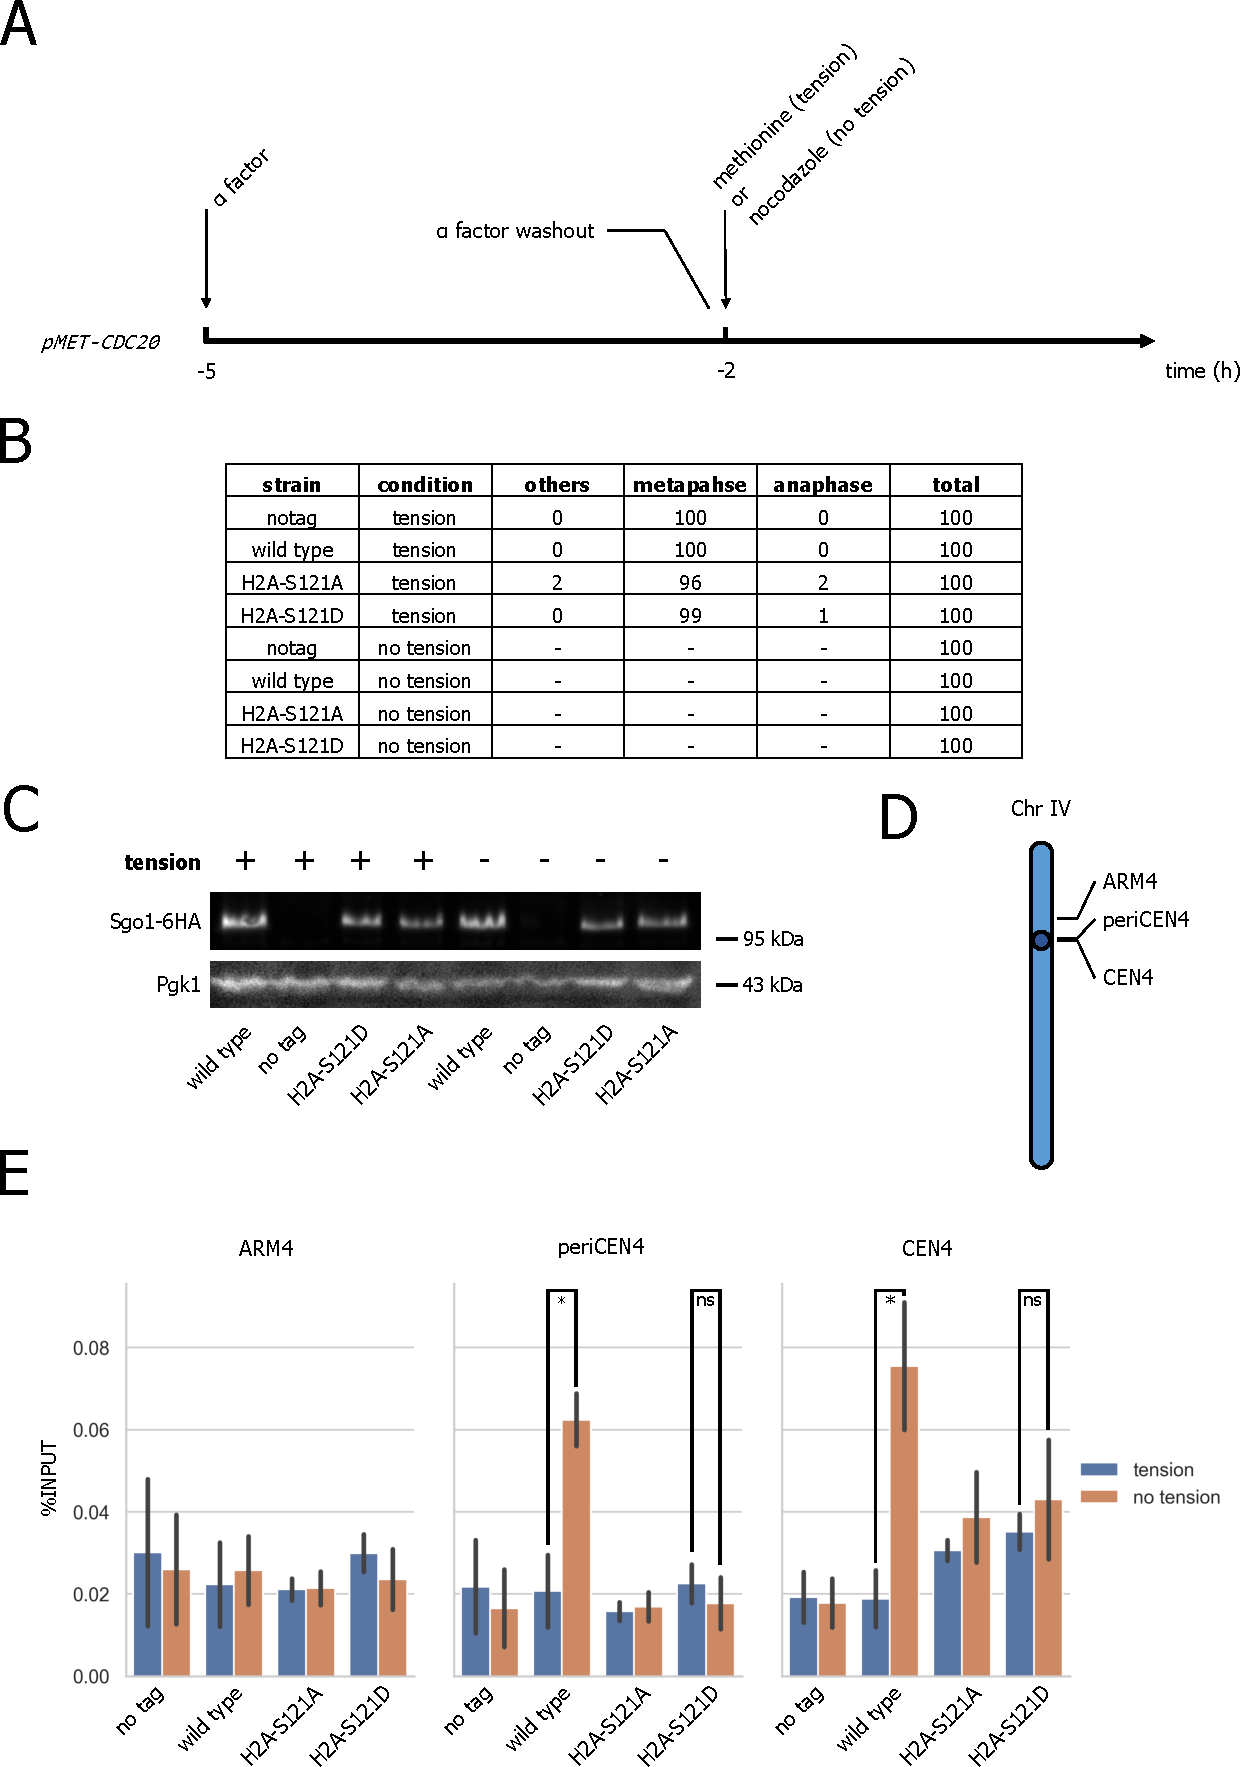
\includegraphics[width=0.9\textwidth]{chapter3/figures/Sgo1 in H2A mutants ChIP.pdf}
  \caption[Sgo1 association with chromatin remains low regardless of tension in H2A phospho-mimic mutant]{Sgo1 association with chromatin remains low regardless of tension in H2A phospho-mimic mutant. (A) Schematics of experimental procedures. (B) Spindle morphology count by tubulin IF. (C) Western blotting with anti-HA antibody to detect the expression level of Sgo1-6HA. Pgk1 was used as the loading control. (D) Schematics showing the locations of loci used for the ChIP-qPCR experiment. (E) Sgo1-6HA ChIP-qPCR on the chromosome arm, the peri-centromere and the core centromere of chromosome IV. The mean of 3 experimental repeats is shown, with the error bar representing standard error. The two-tailed independent t-test is used to calculate statistical significance. (*) P<0.05; (ns) not significant.}
  \label{fig:sgo1chiph2amutants}
\end{figure}

Due to the apparent contradiction with the previous result, I sought to validate the result with microscopy. Therefore, I constructed H2A mutants bearing genetic constructs for imaging, \textit{SGO1-EGFP MTW1-tdTomato}. Cells were imaged following the standard approach of synchronised G1 to metaphase live-cell imaging (Figure~\ref{fig:sgo1imagingh2amutants}A). Unlike wild type, where Sgo1-EGFP appeared as foci at least once in the cell cycle, both of the H2A phospho-mutants could only show Sgo1-EGFP as a 'cloud' signal (Figure~\ref{fig:sgo1imagingh2amutants}B and C). Again, this 'cloud' signal resembles what it looks like in wild type after the establishment of tension, judged by the separation of kinetochore foci. Western blotting showed similar Sgo1 expression levels in the three strains used, ruling out the possibility that the loss of Sgo1-EGFP foci is because of reduced protein abundance (Figure~\ref{fig:sgo1imagingh2amutants}D). Therefore, I concluded that Sgo1 cannot be concentrated at the peri-centromere in H2A phospho-mimic mutant. 

\begin{figure}[htbp]
  \centering
  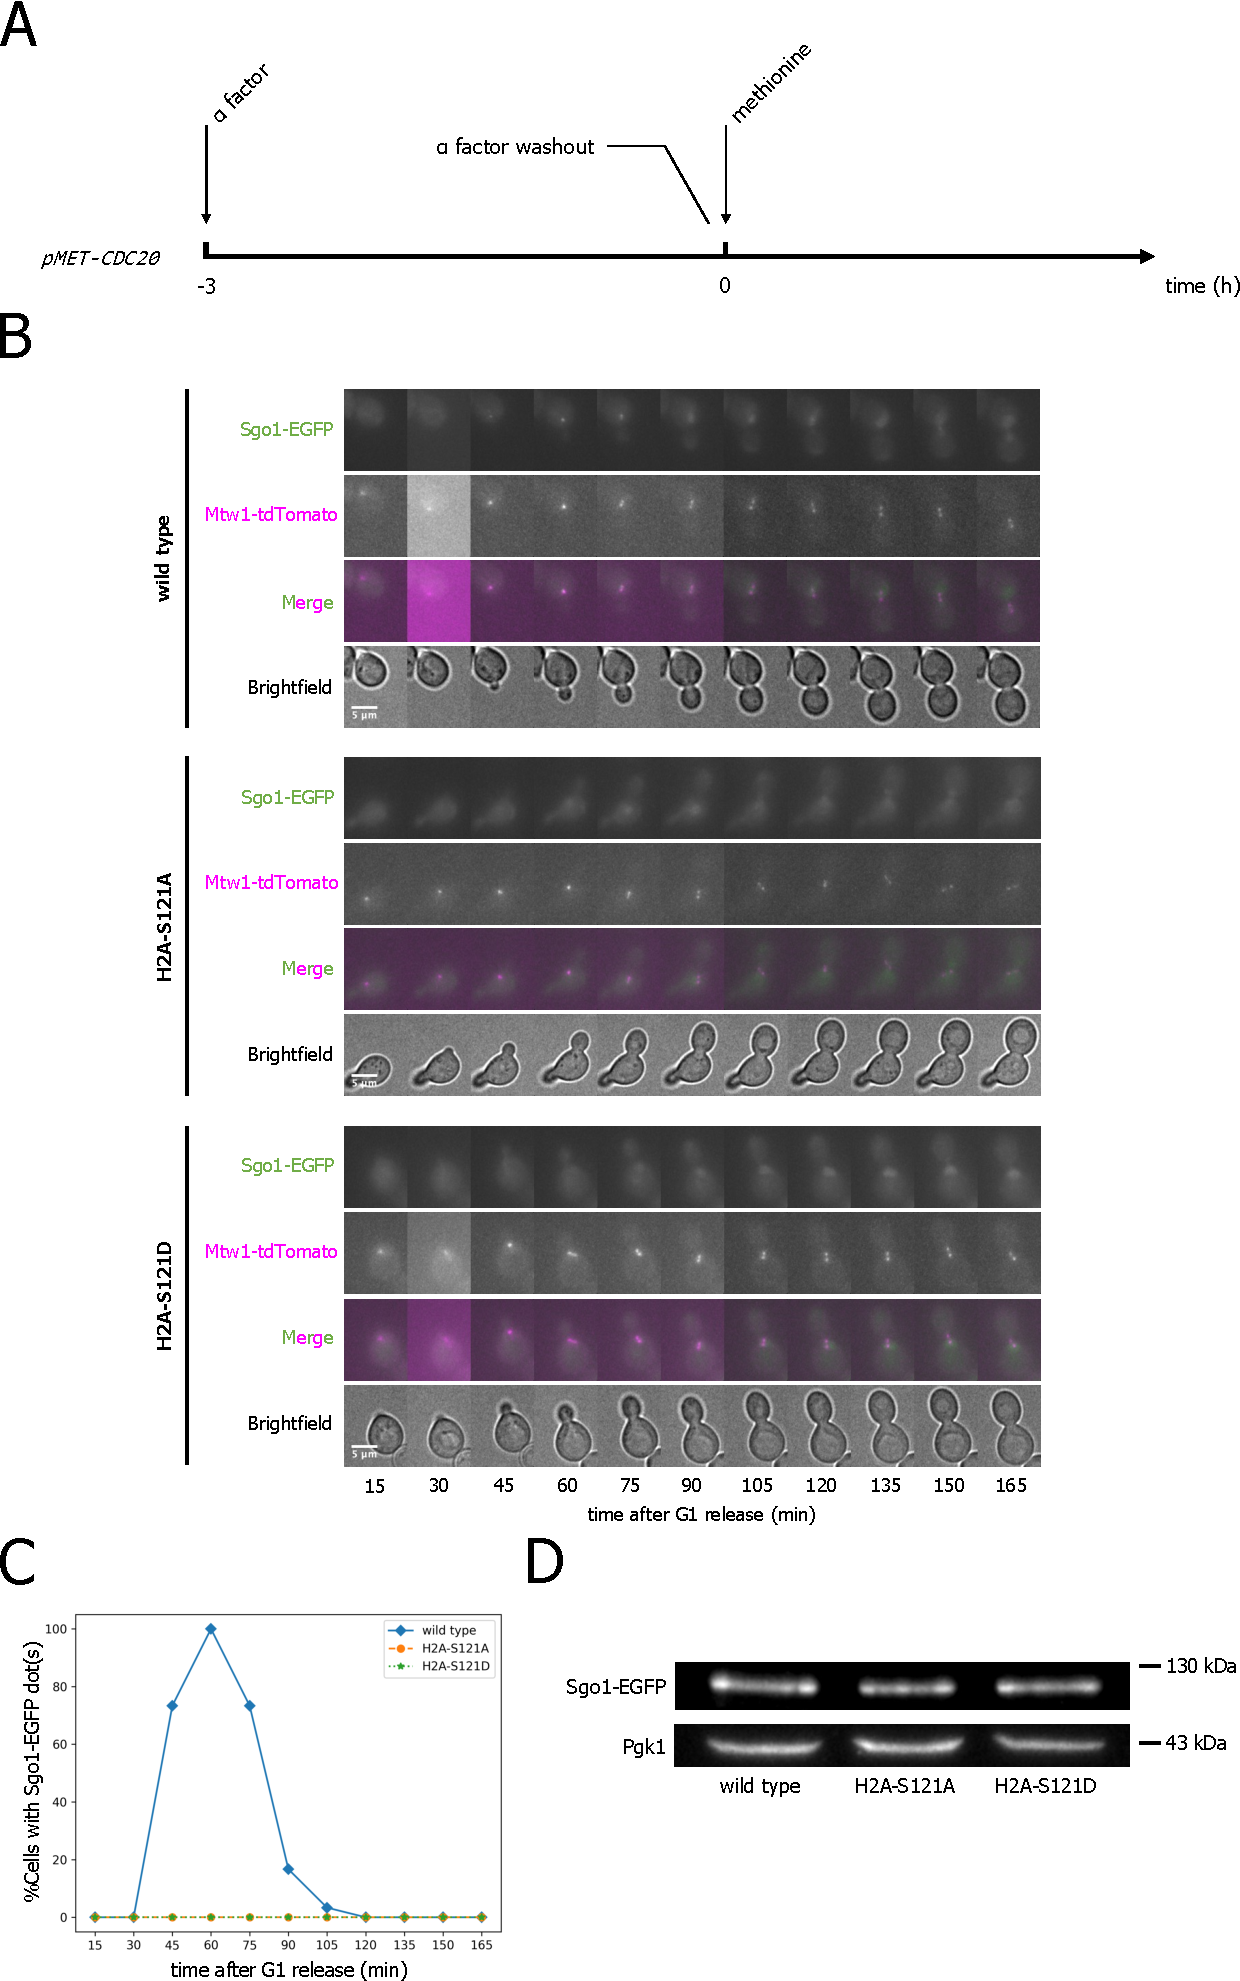
\includegraphics[width=0.9\textwidth]{chapter3/figures/Sgo1 in H2A mutants imaging.pdf}
  \caption[Sgo1 peri-centromere enrichment is abolished in H2A phospho-mimic mutant]{Sgo1 peri-centromere enrichment is abolished in H2A phospho-mimic mutant. (A) Schematics of experimental procedures. (B) Montages of representative time-lapse imaging. (C) N=30 cells for each strain were followed over time and quantified. The percentage of cells with Sgo1 foci was shown as a function of time. (D) Western blotting on cells arrested in metaphase without tension using anti-GFP antibody to detect the expression level of Sgo1-EGFP. Pgk1 was used as the loading control.}
  \label{fig:sgo1imagingh2amutants}
\end{figure}

\subsection{\textit{sgo1$\Delta$} suppresses the growth defect of PP1 temperature-sensitive mutants at their restrictive temperatures}

The working model predicts the existence of one or more phosphatases constantly de-phosphorylating H2A-pS121. We hypothesised PP1 to be one possible candidate. PP1 is a major serine/ threonine phosphatase ubiquitous in eukaryotes and regulates a large number of cellular processes, including SAC silencing and tension sensing \citep{Shi2009Serine/threonineStructure, Cannon2010FunctionCerevisiae, Pinsky2009ProteinYeast, Pinsky2006Glc7/proteinGlc7, London2012, Meadows2011SpindleMotors, Nijenhuis2014NegativeSignal, Rosenberg2011KNL1/Spc105Checkpoint, Liu2010RegulatedKinase, Posch2010Sds22Mitosis, Jin2013TheAttachment}. A functional PP1 enzyme usually consists of a catalytic subunit, which is highly conserved across species, and a regulatory subunit controlling the localisation, substrate specificity, or activity of the catalytic subunit or serves as the substrate itself. The recognition of the catalytic subunit is majorly through the RxVxF motif, and is often accompanied by an additional MyPhoNE or SILK motif \citep{Hendrickx2009DockingPhosphatase-1}. Budding yeast has a single gene encoding the catalytic subunit called \textit{GLC7} \citep{Cannon2010FunctionCerevisiae}. Consistent with its role in SAC silencing, inactivating Glc7 by using temperature-sensitive mutants results in prolonged metaphase arrest and therefore inviability \citep{Andrews2000TypeCerevisiae, MacKelvie1995ThePhosphatase}. 

I started by checking if \textit{SGO1} has genetic interaction with \textit{GLC7}. It has been shown that not allowing Sgo1 re-localisation upon tension by tethering Sgo1 to the kinetochore also arrests cells in metaphase \citep{Su2021SumoylationAnaphase}. If PP1 is the phosphatase that de-phosphorylates H2A-pS121, the growth defect from Glc7 inactivation could be partially attributed to impaired Sgo1 removal. Hence, depleting Sgo1 should be able to relieve it. To test this idea, I constructed double mutants of \textit{sgo1$\Delta$} and \textit{GLC7} temperature-sensitive alleles, either \textit{glc7-10} or \textit{glc7-12}, and carried out spot assay. As reported in previous research \citep{MacKelvie1995ThePhosphatase, Andrews2000TypeCerevisiae}, at their respective restrictive temperatures, 37 \si{\celsius} for \textit{glc7-10} and 34 \si{\celsius} for \textit{glc7-12}, both single mutants were inviable. However, when combined with \textit{sgo1$\Delta$} as double mutants, both strains showed a slight increase in viability (Figure~\ref{fig:growthassay}A), supporting the idea that PP1 is involved in Sgo1 re-localisation from the peri-centromere. 

To verify this result, I wanted to test if \textit{bub1$\Delta$K} mutant, which has unphosphorylated H2A and cannot localise its Sgo1, could phenocopy \textit{sgo1$\Delta$} in restoring the viability of \textit{GLC7} temperature-sensitive mutants. To our surprise, the double mutants indicated the same, if not less, viability compared to \textit{glc7-10} or \textit{glc7-12} single mutant (Figure~\ref{fig:growthassay}B). This finding argues against the hypothesis. However, it has been reported in humans that Bub1 kinase activity is required for cellular processes other than localising Sgo1 \citep{Tang2004, Nyati2015TheSignaling, Li2018TheReplication, Zhang2020FunctioningMitosis}. We reasoned that the loss of other functions of Bub1 kinase might outweigh the benefit of removing Sgo1 from the peri-centromere in the double mutants here. 

\begin{figure}[htbp]
  \centering
  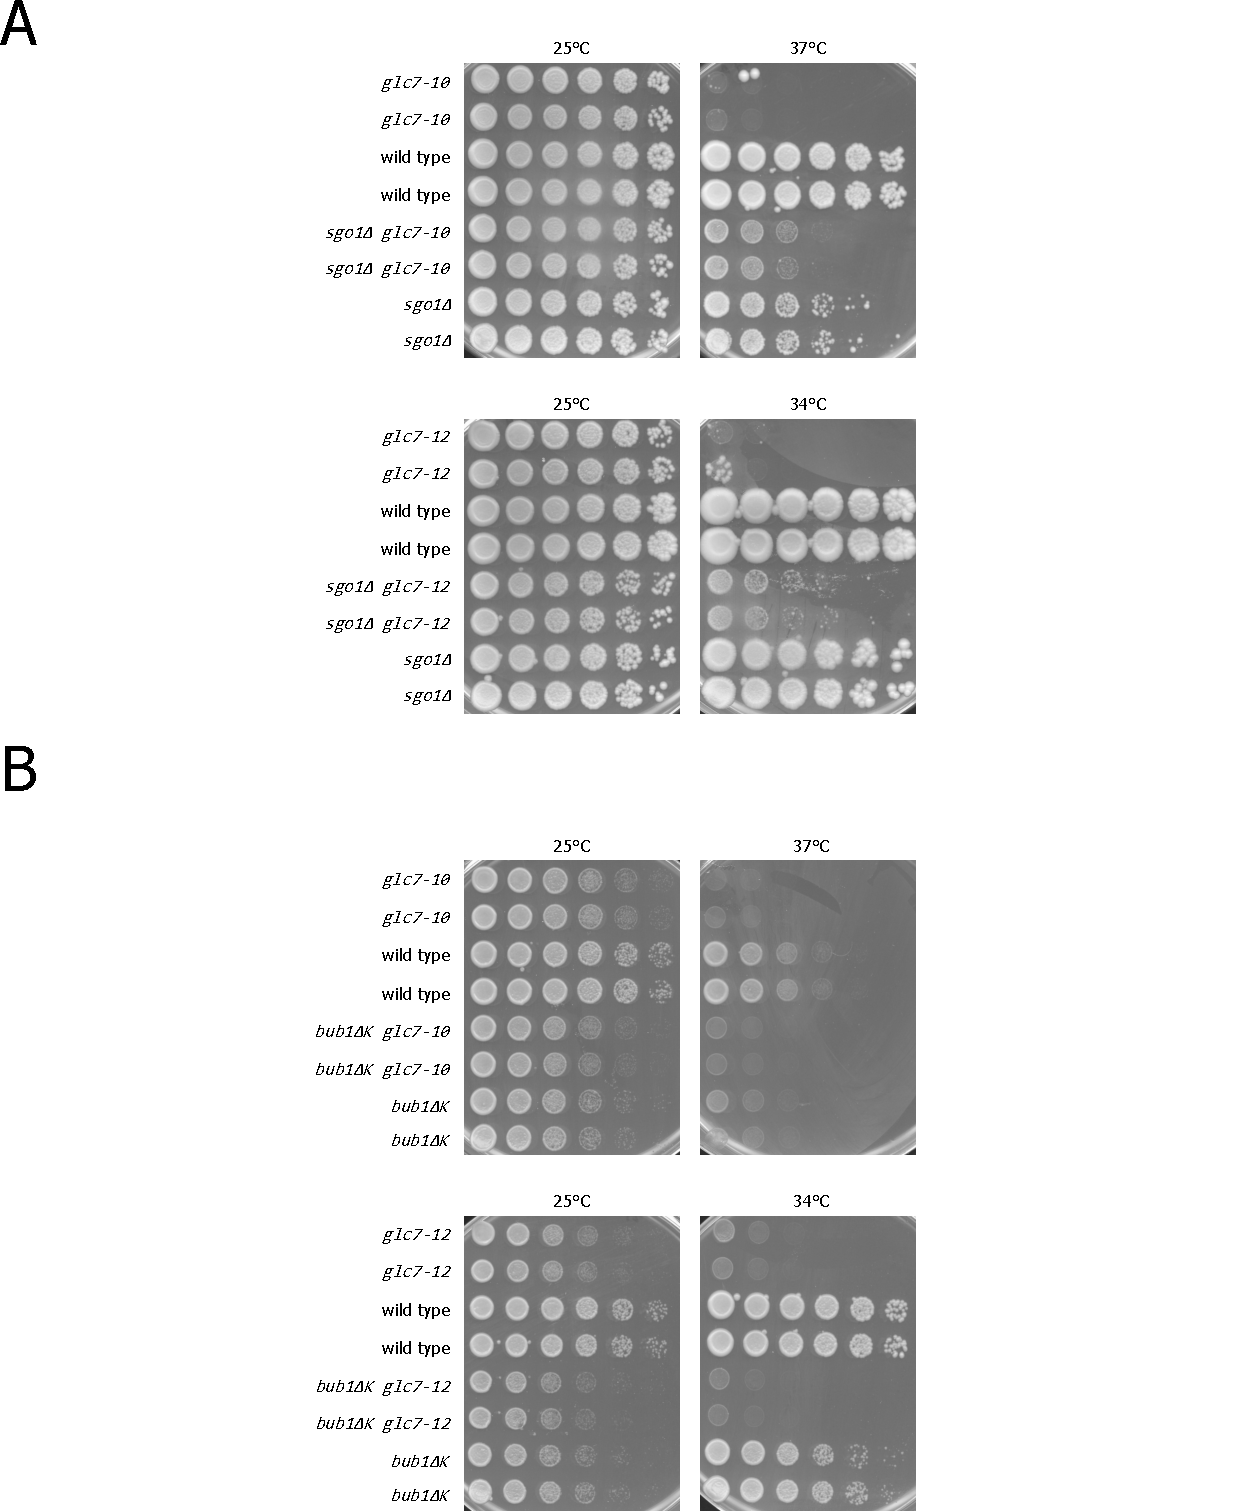
\includegraphics[width=0.9\textwidth]{chapter3/figures/glc7 mutants growth assaay.pdf}
  \caption[\textit{sgo1$\Delta$} but not \textit{bub1$\Delta$K} suppresses the temperature sensitivity of \textit{glc7-10} and \textit{glc7-12} mutant]{\textit{sgo1$\Delta$} but not \textit{bub1$\Delta$K} suppresses the temperature sensitivity of \textit{glc7-10} and \textit{glc7-12} mutant. (A) Serial dilutions of wild type, \textit{sgo1$\Delta$} and \textit{glc7-10} or \textit{glc7-12} single and double mutants spotted on rich medium at room or restrictive temperature. (B) Serial dilutions of wild type, \textit{bub1$\Delta$K} and \textit{glc7-10} or \textit{glc7-12} single and double mutants spotted on rich medium at room or restrictive temperature. The duplications represent technical repeats. }
  \label{fig:growthassay}
\end{figure}

\nomenclature{PP1}{Protein Phosphatase 1}

\subsection{PP1 is required for Sgo1 re-localization}

With the results from the spot assay, I wanted to study the localisation of Sgo1 upon Glc7 inactivation to test whether PP1 is required for Sgo1 removal from the peri-centromere. I first constructed the strain with genetic constructs for Sgo1 imaging (\textit{SGO1-EGFP MTW1-tdTomato pMET-CDC20}) and \textit{glc7-12}, whose restrictive temperature is lower than \textit{glc7-10} and thus might be more compatible with live-cell imaging. the standard G1 to metaphase arrest with tension imaging was conducted except that cells were shifted to 34 \si{\celsius} immediately after G1 release to inactivate PP1 (Figure~\ref{fig:sgo1glc712}A). 

In terms of the inter-kinetochore distance, wild type was similar as in the previous experiments, albeit escaped the arrest induced by Cdc20 depletion near the end of imaging, possibly due to the elevated temperature. Whereas in \textit{glc7-12}, it was stabilised at a much shorter distance, around 0.5 \si{\micro\metre}, over time (Figure~\ref{fig:sgo1glc712}B and C), consistent with the previous report that \textit{glc7-12} cells were arrested in metaphase with short spindles \citep{MacKelvie1995ThePhosphatase}. Interestingly, similar to some of other \textit{GLC7} mutants \citep{Black1995A1, Andrews2000TypeCerevisiae}, many \textit{glc7-12} cells showed elongated bud morphology. The elevated temperature reduced the imaging quality yet the Sgo1-EGFP foci remained distinguishable from the background. Strikingly, in contrast to wild type, Sgo1-EGFP was retained as foci till the end of the experiment in \textit{glc7-12}. Quantification showed that the percentage of \textit{glc7-12} having Sgo1-EGFP foci increased over time and reached nearly 100\% (Figure~\ref{fig:sgo1glc712}B and C), suggesting that Sgo1 cannot be de-localised from the peri-centromere without functional PP1. 

The shortened inter-kinetochore distance in \textit{glc7-12} raised the possibility that Sgo1 is not re-localised because of reduced tension. To test if enough tension was generated in \textit{glc7-12}, I sought to compare the inter-kinetochore distance at which Sgo1 is removed in wild type and the maximum that \textit{glc7-12} could reach. Technically, for individual wild type cell, I identified the first frame that Sgo1-EGFP foci disappeared and recorded its distance between Mtw1-tdTomato foci, which I referred to as wild type$_{removal}$; while for individual \textit{glc7-12} cell, I followed it over time and selected the longest distance its Mtw1-tdTomato foci ever separated, which I named as \textit{glc7-12}$_{maximum}$. As shown in Figure~\ref{fig:sgo1glc712}D, \textit{glc7-12}$_{maximum}$ was slightly larger than wild type$_{removal}$, indicating that \textit{glc7-12} had reached inter-kinetochore distances where Sgo1 is supposed to be de-localised. Therefore, I concluded that the retention of Sgo1 in \textit{glc7-12} cannot be simply explained by the reduced tension. Western blotting further confirmed that this retention is not due to an altered Sgo1-EGFP expression in \textit{glc7-12} (Figure~\ref{fig:sgo1glc712}E). 

\begin{figure}[htbp]
  \centering
  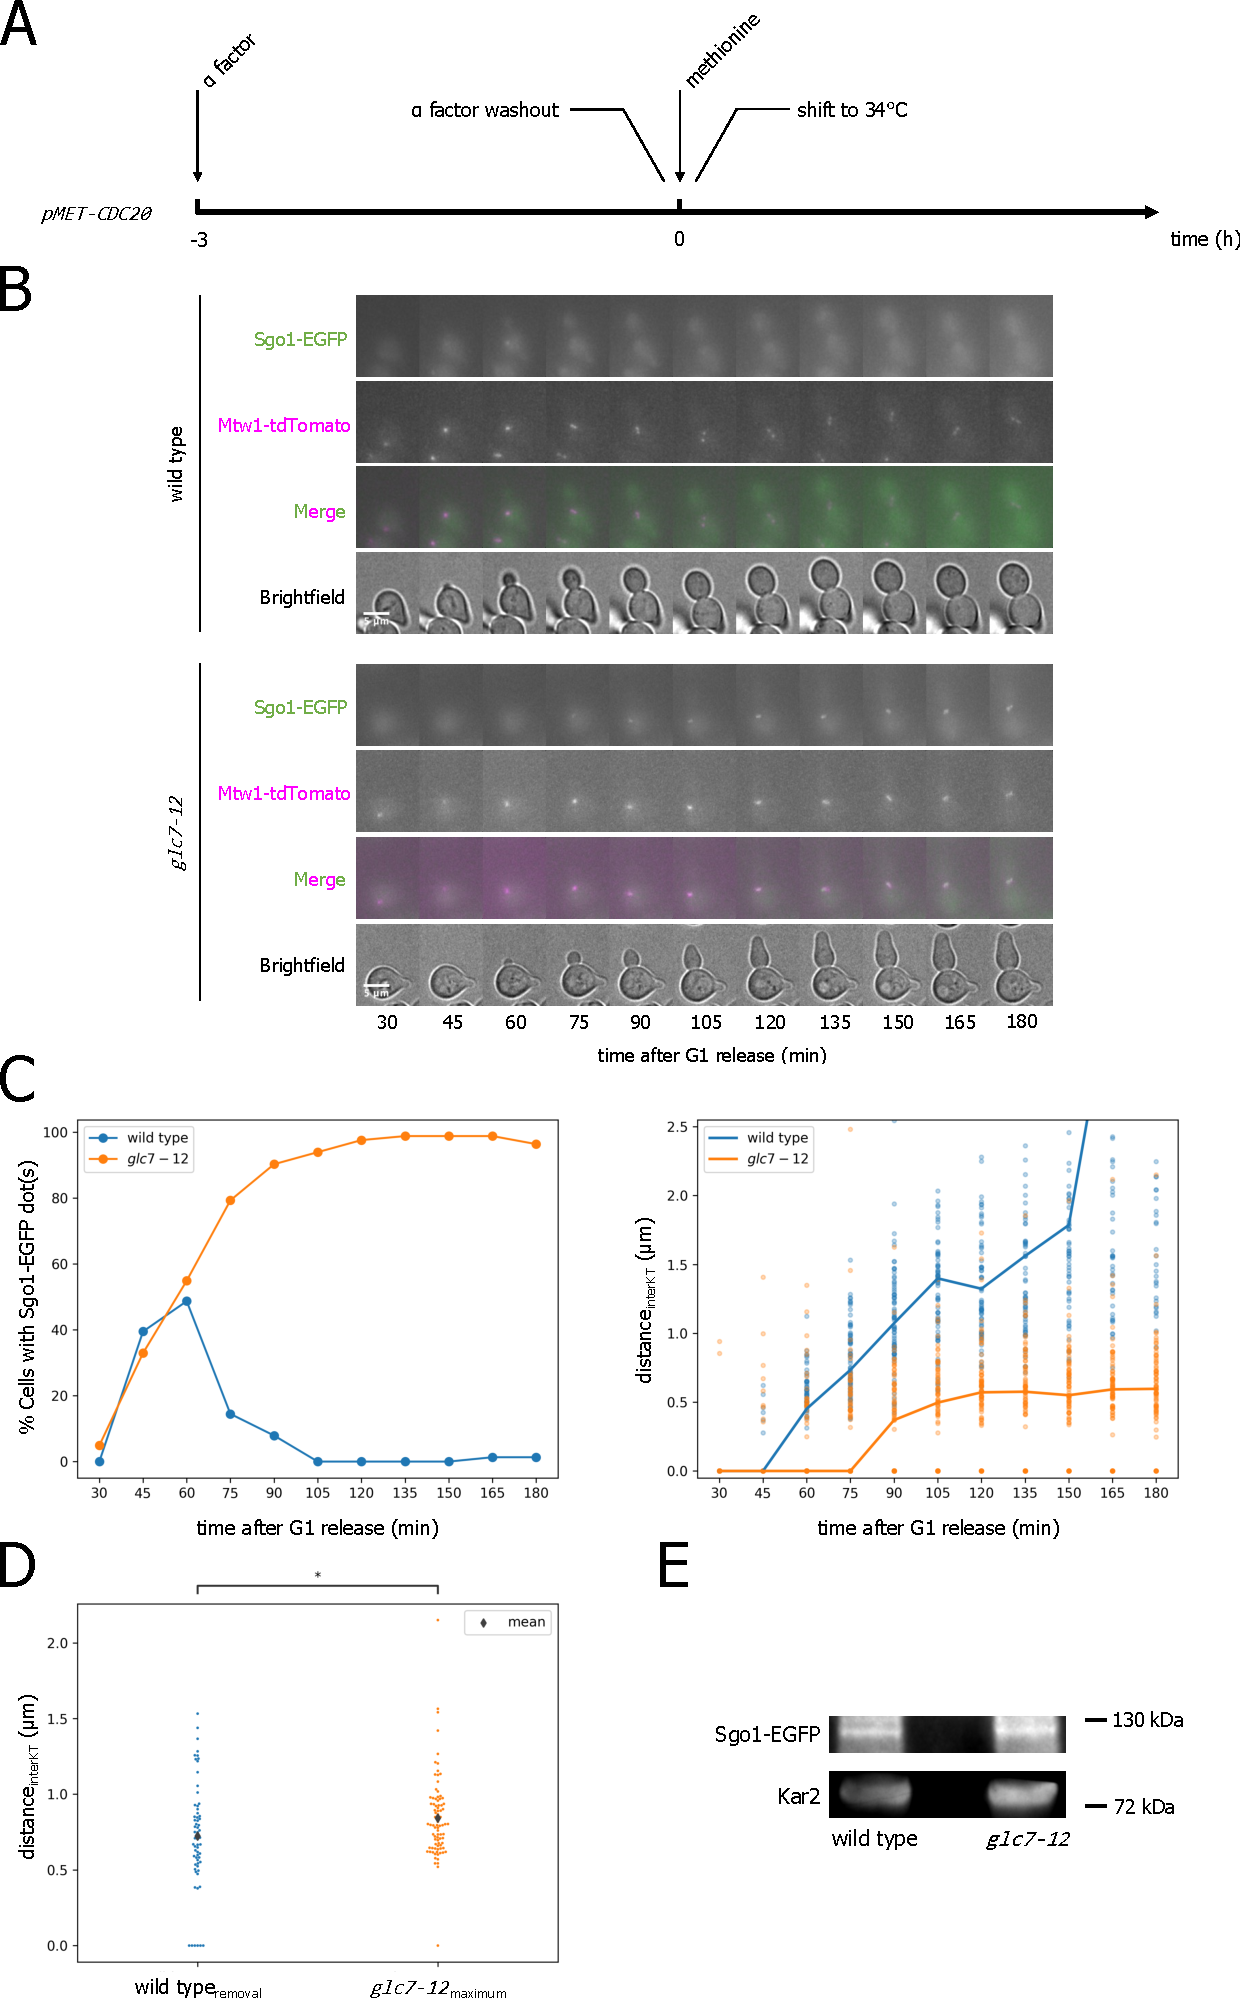
\includegraphics[width=0.9\textwidth]{chapter3/figures/Sgo1 glc7-12.pdf}
  \caption[Sgo1 is not de-localised from peri-centromere in \textit{glc7-12} at restrictive temperature]{Sgo1 is not de-localised from peri-centromere in \textit{glc7-12} at restrictive temperature. (A) Schematics of experimental procedures. (B) Montages of representative time-lapse imaging. (C) N=100 cells for each strain were followed over time and quantified. Top panel: the percentage of cells with Sgo1 foci was shown as a function of time. Bottom panel: median inter-kinetochore distance as a function of time. Individual data points are shown as dots. (D) Comparison between the inter-kinetochore distance at which Sgo1 is removed in wild type (wild type$_{removal}$) and the maximum that \textit{glc7-12} could reach (\textit{glc7-12}$_{maximum}$). The two-tailed independent t-test was used to calculate statistical significance. (*) P<0.05 (E) Western blotting on cells arrested in metaphase without tension using anti-GFP antibody to detect the expression level of Sgo1-EGFP. Kar2 was used as the loading control.}
  \label{fig:sgo1glc712}
\end{figure}

To verify the result, I repeated the experiment in \textit{glc7-10} background (Figure~\ref{fig:sgo1glc710}A). Consistently, Sgo1-EGFP was maintained as foci within the scope of the experiment (Figure~\ref{fig:sgo1glc710}B), supporting the conclusion that PP1 is required for Sgo1 re-localisation. Notably, this experiment's imaging quality was better compared to the one for \textit{glc7-12}. This is unexpected as it was conducted at an even higher temperature. I suspect it might be related to the fact there is immersion oil optimised for imaging at 37 \si{\celsius} but not 34 \si{\celsius}. 

\begin{figure}[htbp]
  \centering
  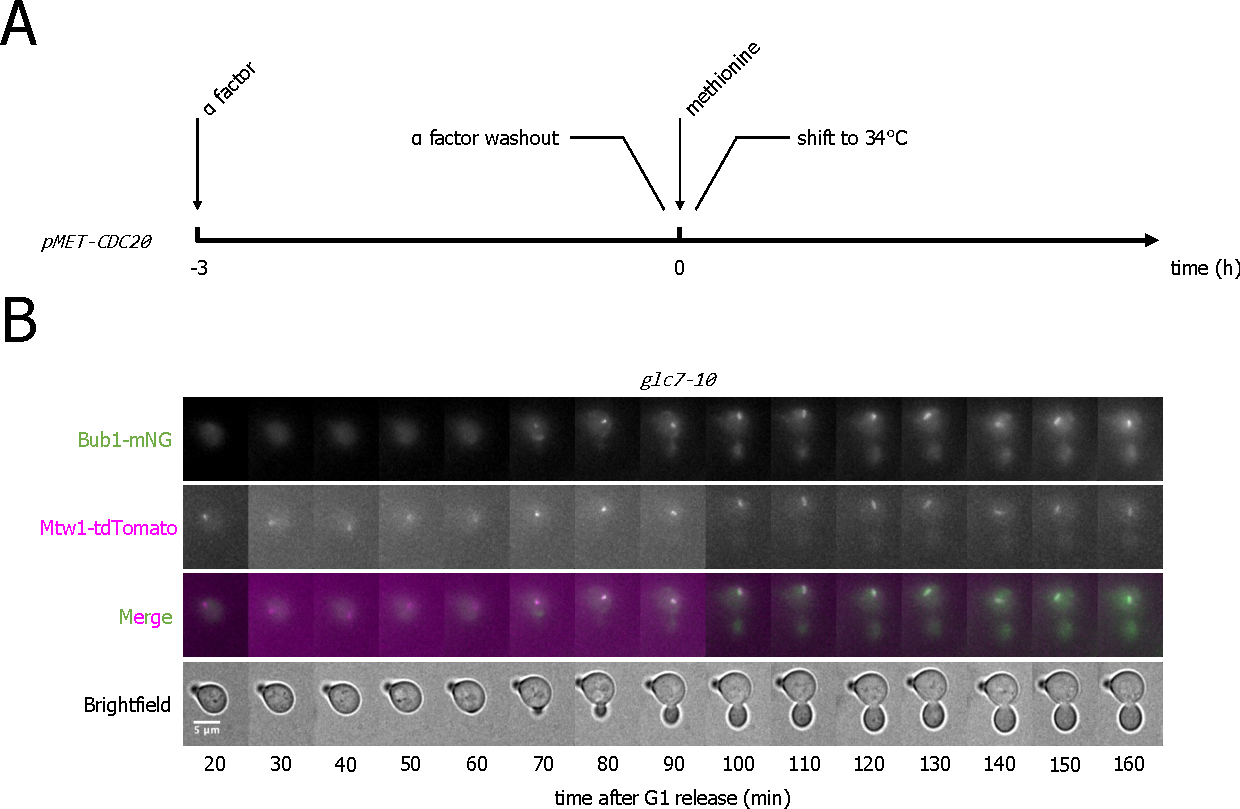
\includegraphics[width=0.9\textwidth]{chapter3/figures/Sgo1 glc7-10.pdf}
  \caption[Sgo1 is not de-localised from peri-centromere in \textit{glc7-10} at restrictive temperature]{Sgo1 is not de-localised from peri-centromere in \textit{glc7-10} at restrictive temperature. (A) Schematics of experimental procedures. (B) Montages of representative time-lapse imaging.}
  \label{fig:sgo1glc710}
\end{figure}

\subsection{PP1-inactivation-caused retention of Sgo1 depends on Bub1}

Next, we wondered whether PP1 is the phosphatase counteracting Bub1 in terms of localising Sgo1. If so, we expected that Sgo1 localisation should be maintained in the absence of both Bub1 and PP1 (Figure~\ref{fig:bub1aidglc712}B). To test this idea, I repeated the 
Bub1 depletion experiment of Figure~\ref{fig:bub1aid} but in the \textit{glc7-12} genetic background. Cells were synchronised in G1 at RT and released to media containing methionine and nocodazole at the restrictive temperature for a metaphase arrest with inactivated PP1 and no tension. NAA was then added to deplete Bub1. Microscopy was used to monitor the localisation of Sgo1 (Figure~\ref{fig:bub1aidglc712}A). Cells showed abnormal bud morphology, indicating successful inactivation of PP1. Unlike the control, Sgo1-EGFP quickly lost its foci signal in the +NAA group with similar dynamics to the previous experiment in Figure~\ref{fig:bub1aid} (Figure~\ref{fig:bub1aidglc712}C and D), suggesting PP1 does not directly counteract Bub1 to de-localise Sgo1. The depletion of Bub1 was not checked in this experiment because Sgo1 peri-centromere localisation was abolished when NAA was added, indicating that Bub1 was depleted as expected. 

\begin{figure}[htbp]
  \centering
  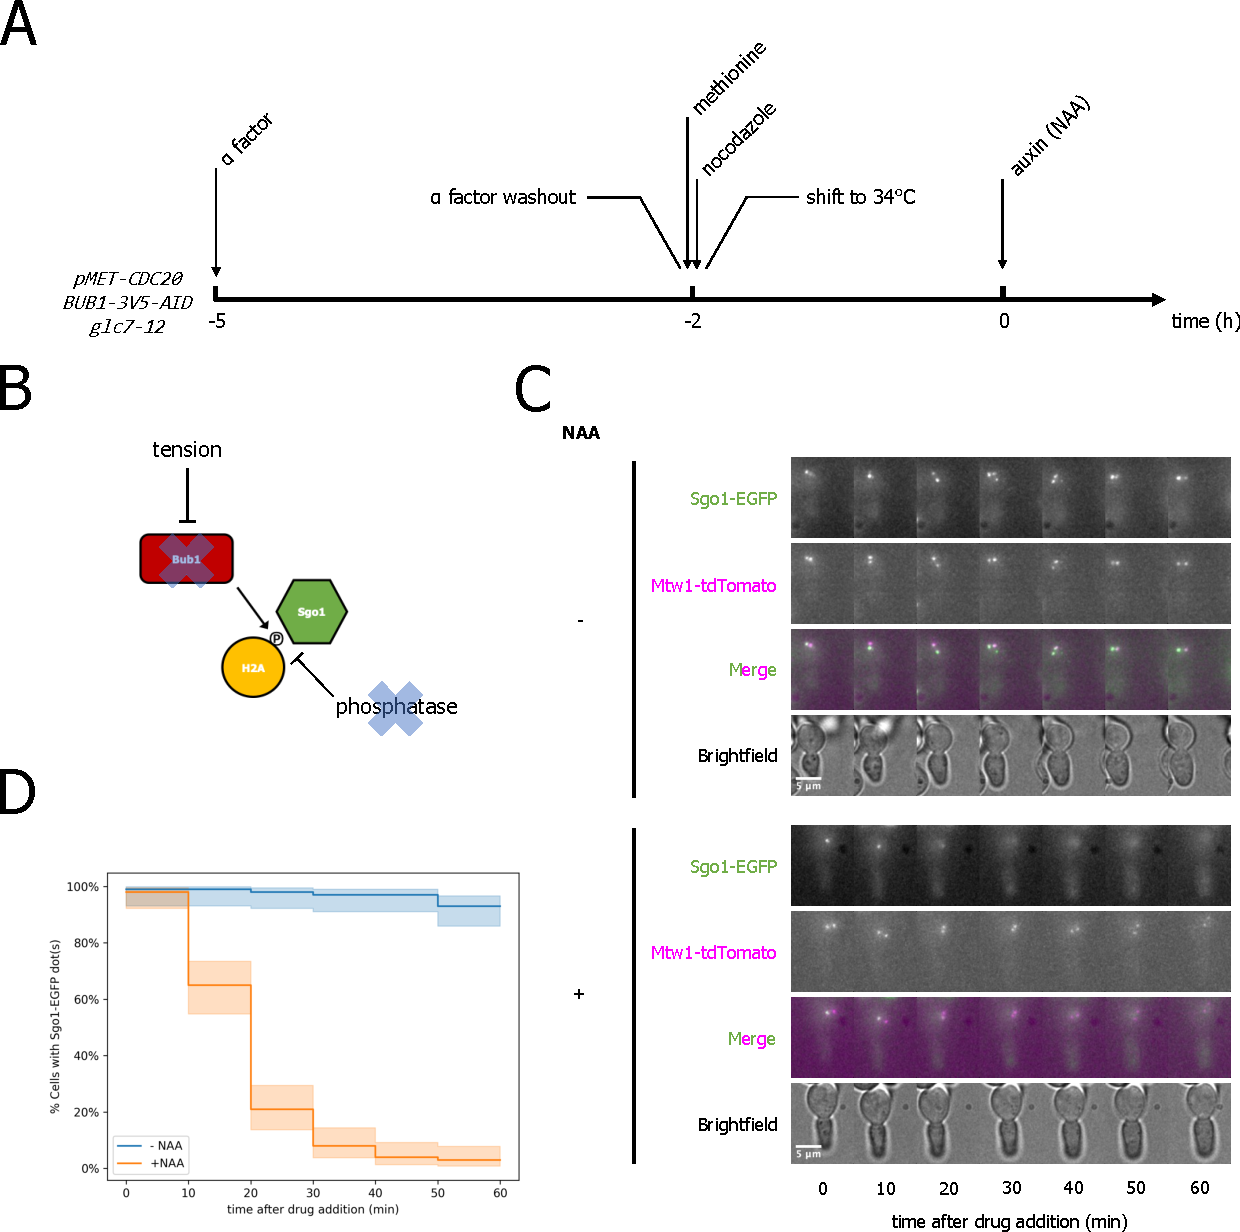
\includegraphics[width=0.9\textwidth]{chapter3/figures/Bub1-AID glc7-12.pdf}
  \caption[PP1 inactivation does not rescue the prompt de-localisation of Sgo1 upon Bub1 depletion in the absence of tension.]{PP1 inactivation does not rescue the prompt de-localisation of Sgo1 upon Bub1 depletion in the absence of tension. (A) Schematics of experimental procedures. (B) Schematics of experimental concept. (C) Montages of representative time-lapse imaging. (D) Survival analysis of the duration of focused Sgo1-EGFP signal. N=30 cells for each strain were followed over time and quantified for the duration of the Sgo1-EGFP signal being focused. Solid lines are Kaplan-Meier survival estimates. The shaded area in the same colour is the 95\% confidence limit of the estimate.}
  \label{fig:bub1aidglc712}
\end{figure}

\subsection{PP1 is required for Bub1 re-localization}

 It has been reported in budding yeast that PP1 could de-phosphorylate the MELT motifs of Spc105, the ortholog of human KNL1, which are important for Bub1 kinetochore localisation \citep{London2012, Roy2019}. We reasoned that the observation that Sgo1 cannot be de-localised upon PP1 inactivation could be due to the retention of Bub1 at the kinetochore in the same condition. To verify this idea, I wanted to study the localisation of Bub1 when PP1 is inactivated. A synchronised G1 to metaphase live-cell imaging at the restrictive temperature of \textit{glc7-12} was performed (Figure~\ref{fig:bub1glc712}A). In wild type, the dynamics of kinetochore-localised Bub1-mNG was as previously described, which was largely reduced at 75 \si{\minute} after G1 release, corresponding to the separation of Mtw1-tdTomato foci. As expected, the drop was not observed in \textit{glc7-12} (Figure~\ref{fig:bub1glc712}B and C), indicating Bub1 de-localisation from the kinetochore upon tension is impaired when PP1 is inactivated. Consistent with the previous experiment, the stabilised inter-kinetochore distance in \textit{glc7-12} was about 0.5 \si{\micro\metre}. Western blotting indicated reduced Bub1 expression in \textit{glc7-12} compared to wild type, probably due to cell death and poorer cell cycle synchronisation. However, it still ruled out the possibility that the increased kinetochore Bub1-mNG fluorescence intensity was because of elevated Bub1 protein level in \textit{glc7-12}. Therefore, combined with the result in the previous section, I concluded that PP1 is required for Sgo1 re-localization due to its role in de-localising Bub1 from the kinetochore. 

\begin{figure}[htbp]
  \centering
  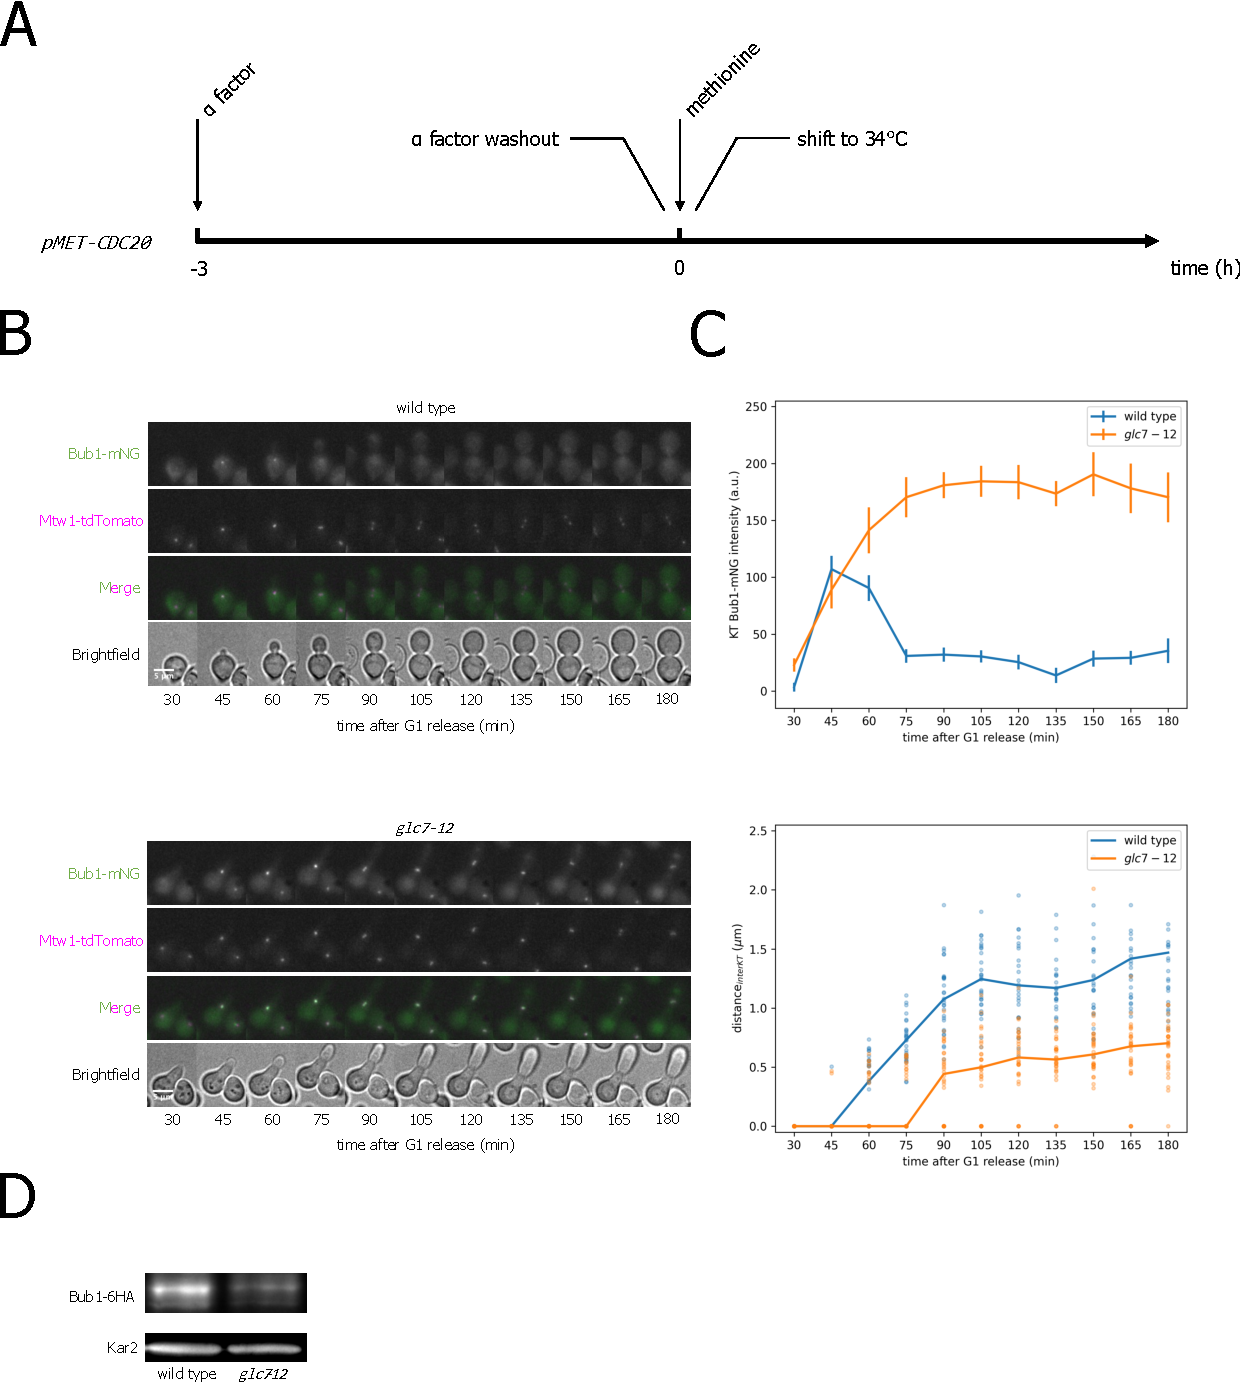
\includegraphics[width=0.9\textwidth]{chapter3/figures/Bub1 glc7-12.pdf}
  \caption[Kinetochore-localised Bub1 is maintained upon PP1 inactivation]{Kinetochore-localised Bub1 is maintained upon PP1 inactivation. (A) Schematics of experimental procedures. (B) Montages of representative time-lapse imaging. (C) N=30 cells were followed over time and quantified for kinetochore Bub1-mNG fluorescence intensity and inter-kinetochore distance. Top panel: mean fluorescence intensity of Bub1-mNG at the kinetochore as a function of time. The error bar represents the standard error. Bottom panel: Median inter-kinetochore distance as a function of time. Individual data points are shown as dots. (D) Western blotting on cells arrested in metaphase without tension using anti-HA antibody to detect the expression level of Bub1-6HA. Kar2 was used as the loading control.}
  \label{fig:bub1glc712}
\end{figure}

\subsection{Putative PP1 binding motifs of Sgo1 are not required for Sgo1 re-localization}

Interestingly, the budding yeast Sgo1 protein sequence contains the consensus PP1 recognition motif RxVxF and the assisting motif SILK, making it a possible regulatory subunit of PP1 (Figure~\ref{fig:sgo1phosphomutant}A). Given the necessity of PP1 in re-localising Sgo1, we hypothesised that the putative interaction between Sgo1 and PP1 could be the key. To test it, we mutated each or both of the motifs and conducted our standard synchronised G1 to metaphase live-cell imaging (Figure~\ref{fig:sgo1phosphomutant}B). Unexpectedly, in all three mutants, the time Sgo1-EGFP spent as foci were not significantly different from wild type (Figure~\ref{fig:sgo1phosphomutant}C), suggesting these motifs are not required for Sgo1 re-localisation. I further tested the functionality of Sgo1 in the mutants by measuring their benomyl sensitivity. In budding yeast, abnormality in SAC or chromosome segregation does not lead to severe growth defects in an undisturbed cell cycle. However, when challenged by the microtubule de-polymerising drug benomyl, it dramatically reduces the viability. As shown in Figure~\ref{fig:sgo1phosphomutant}D, the negative control \textit{sgo1$\Delta$} showed increased sensitivity to benomyl compared to wild type, representing the loss of Sgo1 functions in mitotic chromosome segregation. On the contrary, the mutants did not show an observable reduction in viability in the presence of benomyl, suggesting Sgo1 functions are intact in those strains. Due to the fact that all the mutants' Sgo1 was tagged by EGFP, I added an additional control \textit{SGO1-EGFP} to test if tagging EGFP itself can cause any change in Sgo1 functions. The similar sensitivity to benomyl between \textit{SGO1-EGFP} and wild type suggested a negative answer to the question. Therefore, I concluded that neither timely re-localisation nor the function of Sgo1 requires its putative PP1 binding sites. 

\begin{figure}[htbp]
  \centering
  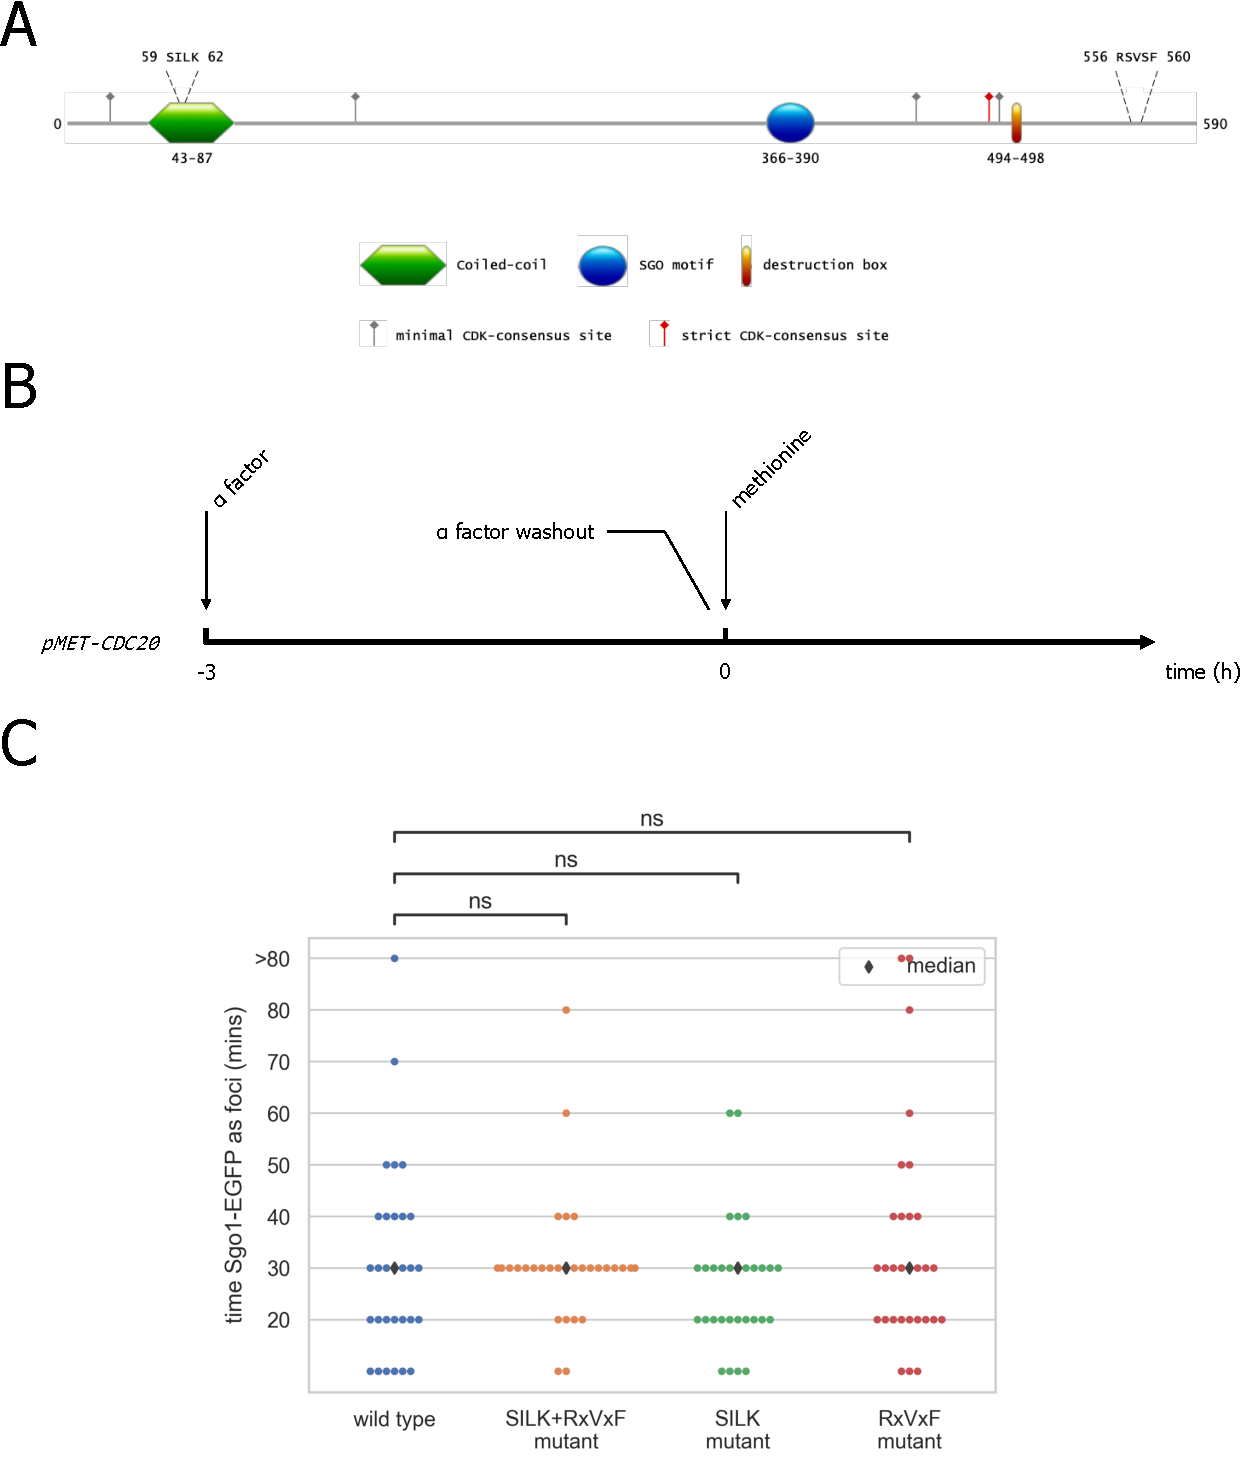
\includegraphics[width=0.9\textwidth]{chapter3/figures/Sgo1 putative PP1 binding mutants.pdf}
  \caption[Neither timely re-localisation nor the function of Sgo1 requires its putative PP1 binding sites]{Neither timely re-localisation nor the function of Sgo1 requires its putative PP1 binding sites. (A) Linear schematics of budding yeast Sgo1 protein. Putative PP1 binding motifs SILK and RSVSF are located at amino acid positions 59-62 and 556-560, respectively. (B) Schematics of the imaging experiment. (C) Quantification of the time of Sgo1-EGFP signal being visualised as foci. The two-tailed independent t-test was used to calculate statistical significance. (*) P<0.05; (ns) not significant. (D) Spot assay testing the benomyl sensitivity of the strains. Serial dilutions of indicated strains spotted on rich medium with 0 or 10 \si{\micro\gram/\micro\litre} benomyl.}
  \label{fig:sgo1phosphomutant}
\end{figure}

\subsection{PP2A-Rts1 might regulate Sgo1 phosphorylation}

Another attempt to identify the phosphatase involved in the re-localisation of Sgo1 focused on PP2A-Rts1. 

PP2A-Rts1 introduction

The commitment to investigating PP2A-Rts1 was decided before the re-establishment of the importance of H2A-pS121 in the process. Instead, we were interested in the possibility that Sgo1 post-translational modifications regulated by PP2A-Rts1 are the key to its localisation. 

Sgo1 PTM introduction

\begin{figure}[htbp]
  \centering
  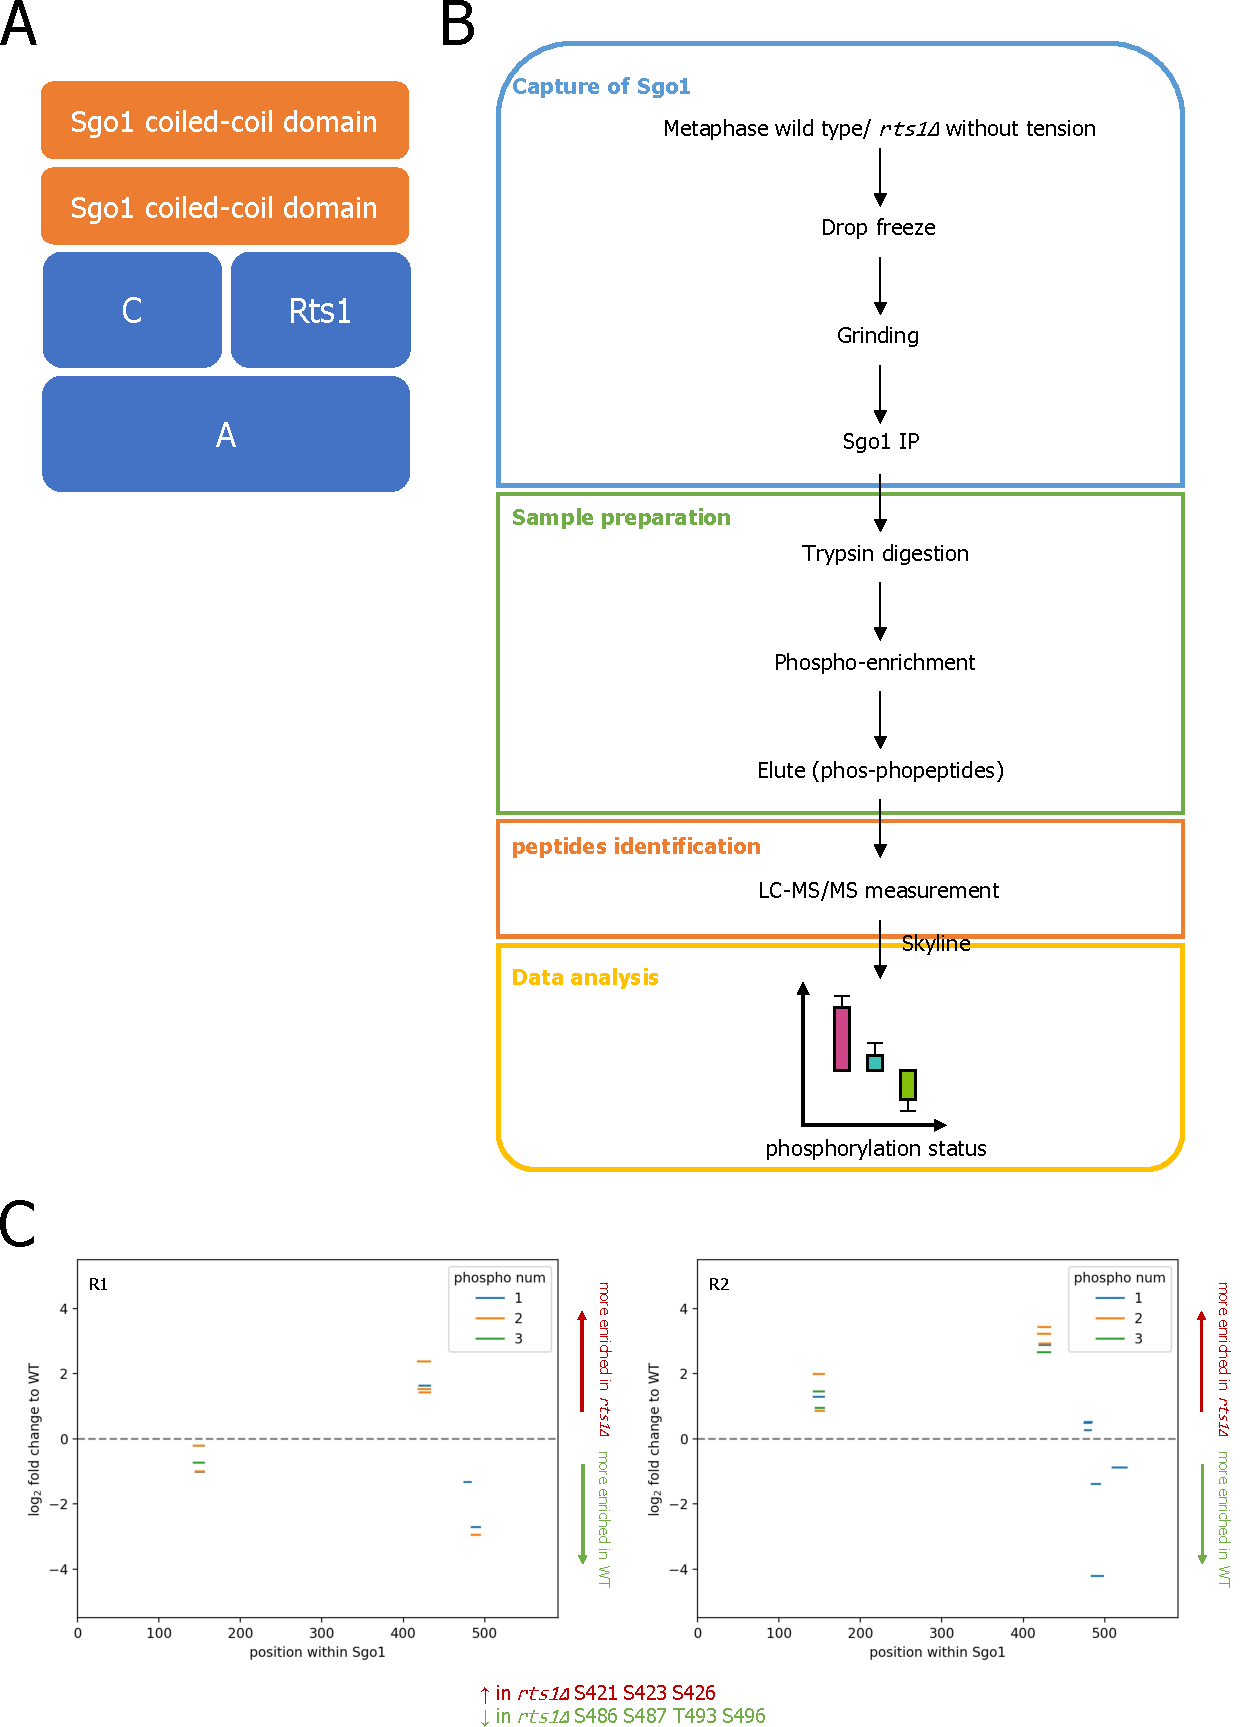
\includegraphics[width=0.9\textwidth]{chapter3/figures/Sgo1 phospho in rts1d.pdf}
  \caption[IP-MS detected changes in Sgo1 phosphorylation in the absence of Rts1]{IP-MS detected changes in Sgo1 phosphorylation in the absence of Rts1. }
  \label{fig:sgo1phosphorts1d}
\end{figure}
\subsection{Sgo1 re-localization is independent of the phosphorylation of S421 or S487}
\begin{figure}[htbp]
  \centering
  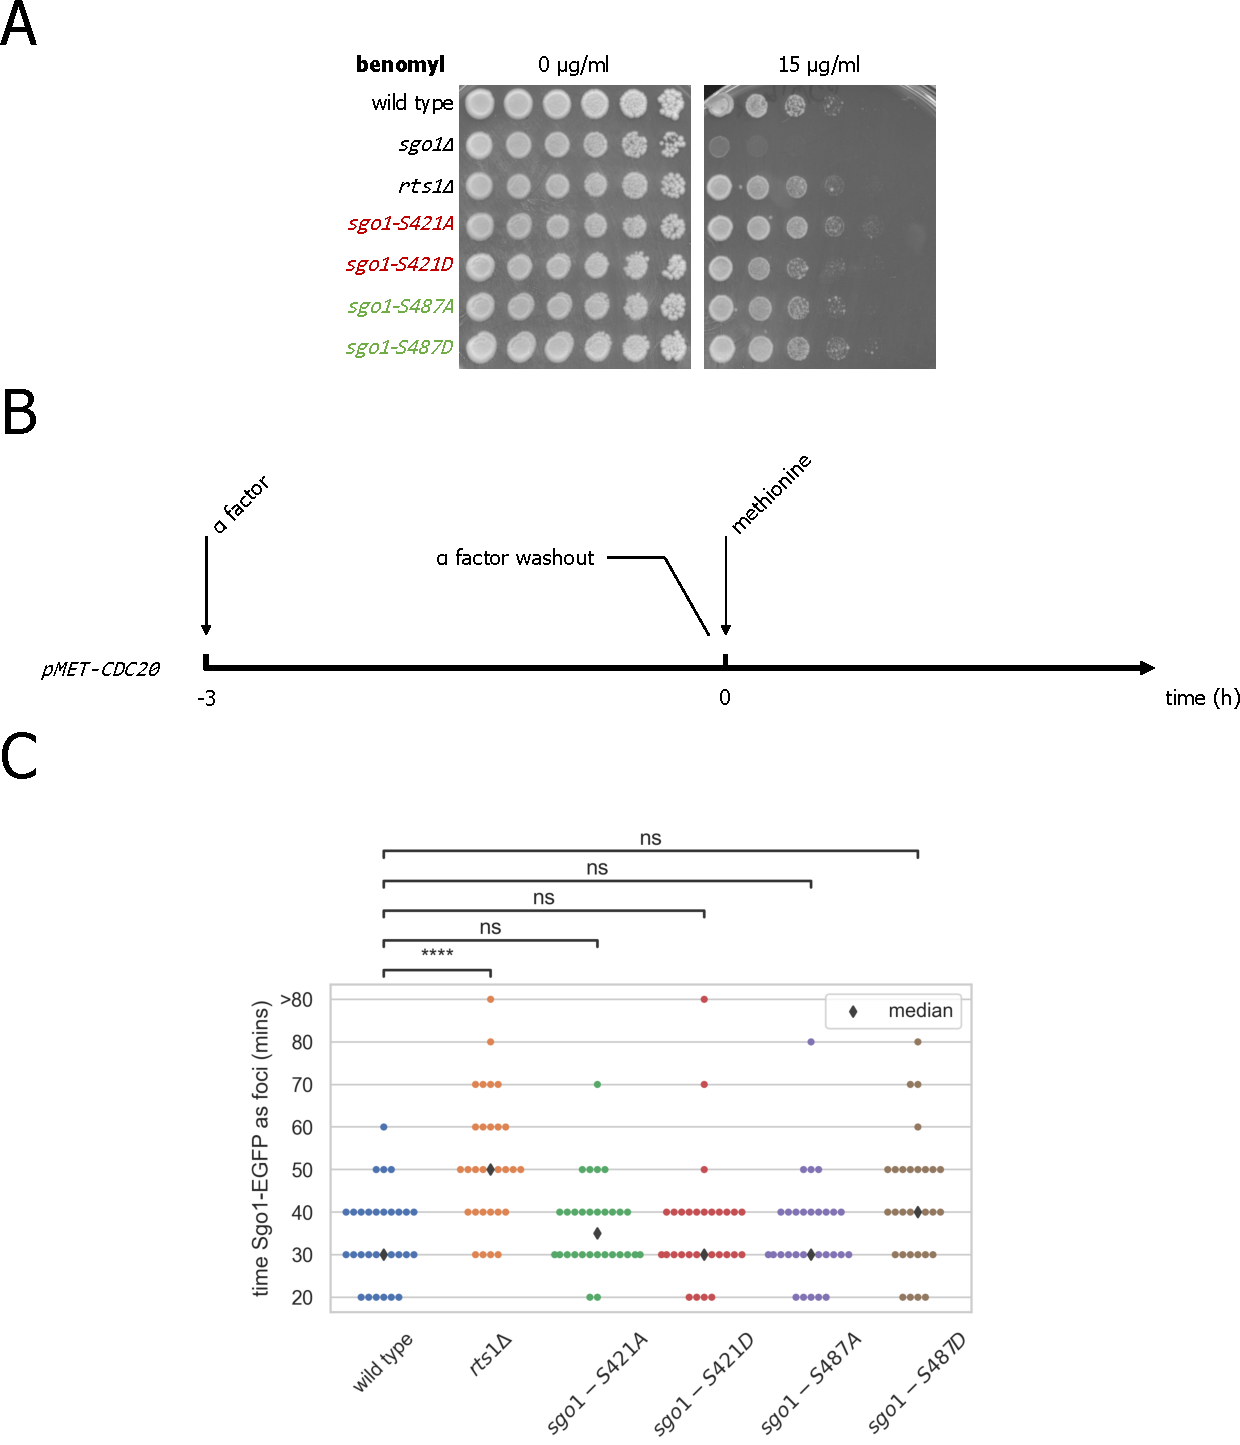
\includegraphics[width=0.9\textwidth]{chapter3/figures/sgo1 phospho mutants.pdf}
  \caption[Phenotypical characterisation of \textit{sgo1} putative Rts1 regulating site phospho-mutants]{Phenotypical characterisation of \textit{sgo1} putative Rts1 regulating site phospho-mutants. }
  \label{fig:sgo1phosphomutants}
\end{figure}
\subsection{PP2A-Rts1 is required for timely sister kinetochore separation}
\begin{figure}[htbp]
  \centering
  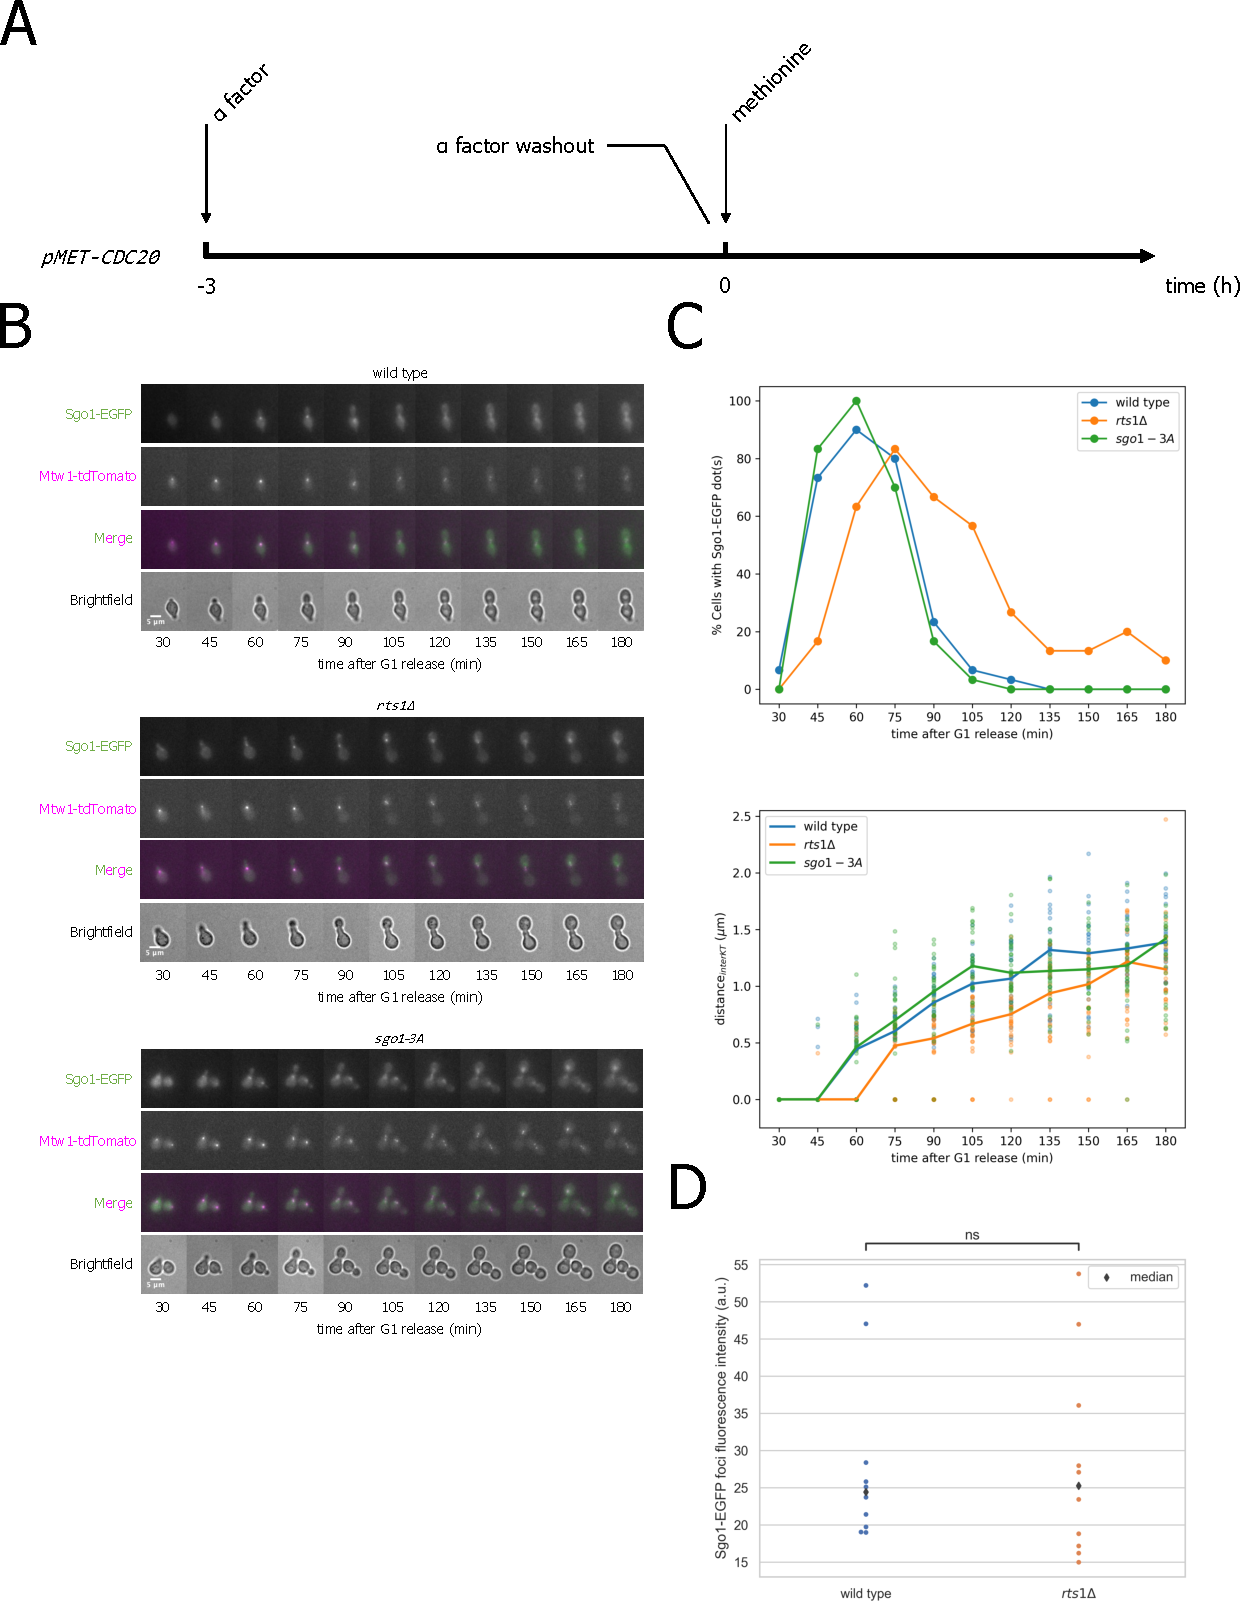
\includegraphics[width=0.9\textwidth]{chapter3/figures/Sgo1 rts1 mutants.pdf}
  \caption[PP2A-Rts1 is required for timely sister kinetochore separation but not for reducing Sgo1 level at peri-centromere]{PP2A-Rts1 is required for timely sister kinetochore separation but not for reducing Sgo1 level at peri-centromere. }
  \label{fig:sgo1rts1mutants}
\end{figure}
\subsection{Tension increases long-range \textit{in cis} interactions}
\subsection{Cohesin is not required for the concentration of Sgo1 at the peri-centromere}

In the absence of tension, the association of Sgo1 with chromatin shows three major peaks, at the core centromere and the two peri-centromere borders \citep{Verzijlbergen2014, Paldi2020ConvergentPericentromeres}. Intriguingly, this is different from H2A-pS121, whose distribution profile is rather bell-shaped (Figure~\ref{fig:sgo1comparison}). Given its necessary role in localising Sgo1, this result is quite surprising and it suggests that there might be other factors determining Sgo1 localisation. It has been shown in humans that interaction with cohesin is key to Sgo1 localisation at the inner centromere \citep{Liu2013a}. Also, in budding yeast, cohesin depletion results in a reduction in the ChIP signal at the centromeric region \citep{Verzijlbergen2014}. Therefore, we hypothesised that cohesin might be the other factor involved in defining the distribution of Sgo1 here. 

\begin{figure}[htbp]
  \centering
  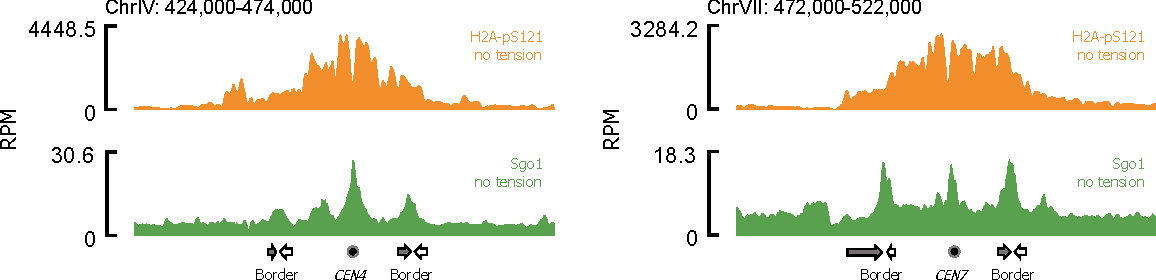
\includegraphics[width=0.9\textwidth]{chapter3/figures/Sgo1 comparison.pdf}
  \caption[H2A-pS121 ChIP-seq profile is qualitatively different from Sgo1]{H2A-pS121 ChIP-seq profile is qualitatively different from Sgo1. ChIP-seq profiles of H2A-pS121 and Sgo1 \citep{Paldi2020ConvergentPericentromeres} at the 50kb regions of chromosome IV and VII centromeres. Convergent genes at the peri-centromere borders are marked as arrows. }
  \label{fig:sgo1comparison}
\end{figure}

\nomenclature{qPCR}{quantitative Polymerase Chain Reaction}
\nomenclature{RPM}{Reads Per Million}

\subsection{Sgo1 acetylation is not required for Sgo1 re-localization}

\section{Discussion}
\section{Materials and methods}
\subsection{Budding yeast methods}
\subsubsection{Strain construction}
\subsection{Microscopy methods}
\subsubsection{FRET}
The FRET experiment was performed on a Nikon Ti2 inverted microscope equipped with a 100x Plan ApoChromat NA 1.45 oil lens and Prime 95B CMOS (sCMOS) camera. Fluorophores were excited with GFP and emission in the mCherry channel was recorded. Subsequently, standard GFP-GFP and mCherry-mCherry excitation and emission were performed. 

bleed-through from both fluorophores to the FRET channel are subtracted in ImageJ using the following formula: 
Acceptor in FRET channel (Co-efficient A) =	Mean intensity of Acceptor using FRET set/ Mean intensity of Acceptor using acceptor set

Donor in FRET channel (Co-efficient B) = Mean intensity of Donor only using FRET filter set/ Mean intensity of Donor only using Donor filter set

FRET Specimen - (A * FRET Specimen using Acceptor filter set) - (B * FRET Specimen using Donor filter set)

Protocol

Use 3 samples

Acceptor Only
Donor Only
FRET Sample
Collect 5 images

Acceptor Only using Acceptor filter set
Acceptor Only using the FRET filter set
Donor Only using the Donor filter set
Donor Only using the FRET filter set
FRET Specimen Only using FRET filter set

reference \citep{Gordon1998QuantitativeMicroscopy}

\subsubsection{Live-cell imaging}
Cells bearing \textit{pMET-CDC20} from patches on -MET plates were inoculated in 10 \si{\milli\litre} of CSM -MET and incubated at RT with shaking at 250 rpm overnight. Cells were diluted to $OD_{600}$=0.2 in 10 \si{\milli\litre} of CSM -MET in the morning, incubating at RT with shaking at 250rpm for over 1 \si{\hour}, allowing cells to enter the exponential phase. Then, cells were re-diluted to $OD_{600}$=0.2 in 10 \si{\milli\litre} of CSM -MET and 10 \si{\micro\litre} of 10 \si{\micro\gram/\milli\litre} alpha factor was added for G1 synchronization. After 1.5 \si{\hour}, another 5 \si{\micro\litre} of 10 \si{\micro\gram/\milli\litre} alpha factor was added. 1.5 \si{\hour} later, shmoo morphology was checked by a light microscope to ensure G1 arrest. 1 \si{\milli\litre} of cell culture was transferred to a 1.5 \si{\milli\litre} Eppendorf tube and concentrated by centrifuging at 3000 rpm for 3 \si{\minute} then removing 700 \si{\micro\litre} of supernatant. 250 \si{\micro\litre} of concentrated cell culture was loaded onto an 8-well Ibidi dish pre-treated with concanavalin A (preparation see separate protocol) and incubated at RT on bench for 15 \si{\minute} to allow cells to bind the bottom of the dish. The supernatant was removed using a bench aspirator and cells were washed twice with 250 \si{\micro\litre} of SC. After the final wash, 250 \si{\micro\litre} of SC was added to each well for imaging. 

\nomenclature{MET}{METhionine}

\subsubsection{Using AID system in microscopy}

\subsubsection{Quantification of fluorescence intensity}

\nomenclature{RT}{Room Temperature}
\nomenclature{rpm}{revolutions per minute}

\subsection{Protein methods}
\subsubsection{Western blotting}
normal protein
H2A-pS121
\subsubsection{Western blotting with big gel}
\subsubsection{Generation of phospho-specific antibody for H2A-pS121}
\subsubsection{ChIP}
for qPCR
for seq
\subsection{DNA methods}
\subsubsection{qPCR}

\begin{table}[htbp]
\centering
\renewcommand{\arraystretch}{1.5}
\caption{qPCR primers}
\label{tab:qpcr}
\resizebox{\textwidth}{!}{%
\begin{tabular}{ccccl}
\hline
\multicolumn{1}{c}{Species}            & \multicolumn{1}{c}{Locus}  & \multicolumn{1}{c}{Direction} & \multicolumn{1}{c}{Number} & \multicolumn{1}{c}{Sequence}                 \\
\hline
\multirow{2}{*}{\textit{S.cerevisiae}} & \multirow{2}{*}{CEN4(a)}   & Forward   & 794    & CCGAGGCTTTCATAGCTTA      \\
                                       &                            & Reverse   & 795    & ACCGGAAGGAAGAATAAGAA     \\
\multirow{2}{*}{\textit{S.cerevisiae}} & \multirow{2}{*}{CEN4(b)}   & Forward   & 8172   & GCCGAGGCTTTCATAGCTTA     \\
                                       &                            & Reverse   & 8173   & GACGATAAAACCGGAAGGAAG    \\
\multirow{2}{*}{\textit{S.cerevisiae}} & \multirow{2}{*}{ARM4}      & Forward   & 8175   & GCTACCACCAATAACACAGTTGAG \\
                                       &                            & Reverse   & 8176   & GTACCTTCCCTGATAATCCGTCT  \\
\multirow{2}{*}{\textit{S.cerevisiae}} & \multirow{2}{*}{peri-CEN4} & Forward   & 8599   & TGTAACGGTCATGGTTGTCTTC   \\
                                       &                            & Reverse   & 8600   & ACCTCATTCGTCATGTGAGAGA   \\
\multirow{2}{*}{\textit{S.pombe}}      & \multirow{2}{*}{CEN}      & Forward   & 2179   & CAGACAATCGCATGGTACTATC   \\
                                       &                            & Reverse   & 2180   & AGGTGAAGCGTAAGTGAGTG     \\
\multirow{2}{*}{\textit{S.pombe}}      & \multirow{2}{*}{OTR}  & Forward   & 2183   & GCGTCGGAAGGTTGAGAATA     \\
                                       &                            & Reverse   & 2184   & CTGCACTAGCAATTGGATCG  
\\
\hline                                                             

\end{tabular}%
}
\end{table}
\nomenclature{OTR}{OuTer Repeat}

\subsubsection{Library preparation for Illumina sequencing}
\subsection{Computational methods}
\subsubsection{ChIP-seq data analysis}
\subsubsection{Code availability}